% ---------------------------------------------------------------
% TEMPLATE TCC2 - SENAC SANTO AMARO
% ---------------------------------------------------------------
% Trabalho de Conclusão de Curso 2
% ---------------------------------------------------------------

\documentclass[
    12pt,                % tamanho da fonte
    openright,           % capítulos começam em página ímpar
    oneside,             % para impressão em apenas um lado do papel
    a4paper,             % tamanho do papel
    english,             % idioma adicional
    brazil               % idioma principal
]{abntex2}

% ---------------------------------------------------------------
% PACOTES
% ---------------------------------------------------------------
\usepackage{lmodern}                % Fonte Latin Modern
\usepackage[T1]{fontenc}            % Seleção de códigos de fonte
\usepackage[utf8]{inputenc}         % Codificação do documento
\usepackage{lastpage}               % Usado pela Ficha catalográfica
\usepackage{indentfirst}            % Indenta o primeiro parágrafo
\usepackage{color}                  % Controle de cores
\usepackage{graphicx}               % Inclusão de gráficos
\usepackage{microtype}              % Melhorias de justificação
\usepackage{float}                  % Para posicionamento de figuras
\usepackage{booktabs}               % Tabelas profissionais
\usepackage{multirow}               % Células mescladas em tabelas
\usepackage{longtable}              % Tabelas longas
\usepackage{amsmath,amssymb}        % Símbolos matemáticos
\usepackage{pgfgantt}               % Diagramas de Gantt
\usepackage[brazilian,hyperpageref]{backref}  % Páginas com citações
\usepackage[alf]{abntex2cite}       % Citações ABNT
\usepackage{tabularx}               % Tabelas

% ---------------------------------------------------------------
% CONFIGURAÇÕES DO PDF
% ---------------------------------------------------------------
\makeatletter
\hypersetup{
    pdftitle={\@title},
    pdfauthor={\@author},
    pdfsubject={TCC2 - Senac Santo Amaro},
    pdfcreator={LaTeX with abnTeX2},
    pdfkeywords={tcc}{senac}{santo amaro}{trabalho de conclusão},
    colorlinks=true,        % false: links em caixas; true: links coloridos
    linkcolor=blue,         % cor dos links internos
    citecolor=blue,         % cor dos links para bibliografia
    filecolor=magenta,      % cor dos links para arquivos
    urlcolor=blue,
    bookmarksdepth=4
}
\makeatother

% ---------------------------------------------------------------
% CONFIGURAÇÕES DE APARÊNCIA DO PDF FINAL
% ---------------------------------------------------------------
\definecolor{blue}{RGB}{41,5,195}

% ---------------------------------------------------------------
% INFORMAÇÕES DO DOCUMENTO
% ---------------------------------------------------------------
\titulo{Classificação Automática de Chamados de TI Utilizando Processamento de Linguagem Natural com Explicabilidade Baseada em Grafos}
\autor{Agatha Barbosa Marinho dos Santos \\
Bruna Kinjo Luiz Pinto \\
Kayke Ahrens Biscegli}
\local{São Paulo}
\data{2026}
\orientador{Prof. Douglas José Baquião Ribeiro}
% \coorientador{Prof. Nome do Coorientador} % Descomente se houver coorientador

\instituicao{%
  Senac -- Serviço Nacional de Aprendizagem Comercial
  \par
  Unidade Santo Amaro
  \par
  Curso de Bacharelado em Ciência da Computação
}

\tipotrabalho{Trabalho de Conclusão de Curso II}

\preambulo{Trabalho de Conclusão de Curso II apresentado ao Senac Santo Amaro como requisito para conclusão do curso de Bacharelado em Ciência da Computação.}

% ---------------------------------------------------------------
% COMPILA O ÍNDICE
% ---------------------------------------------------------------
\makeindex

% ---------------------------------------------------------------
% INÍCIO DO DOCUMENTO
% ---------------------------------------------------------------
% Legenda "Fonte:" em tamanho menor que o texto (ABNT)
\let\legendoriginal\legend
\renewcommand{\legend}[1]{\legendoriginal{\small #1}}
\setlength{\emergencystretch}{3em}
\begin{document}

% Seleciona o idioma do documento
\selectlanguage{brazil}

% Retira espaço extra obsoleto entre as frases
\frenchspacing

% ---------------------------------------------------------------
% ELEMENTOS PRÉ-TEXTUAIS
% ---------------------------------------------------------------
\pretextual

% ---------------------------------------------------------------
% CAPA
% ---------------------------------------------------------------
\imprimircapa

% ---------------------------------------------------------------
% FOLHA DE ROSTO
% ---------------------------------------------------------------
\imprimirfolhaderosto

% ---------------------------------------------------------------
% RESUMO
% ---------------------------------------------------------------
\begin{resumo}
O objetivo deste trabalho é investigar como a inclusão de uma camada de explicabilidade baseada em SHAP, LIME e grafos de co-ocorrência a um \textit{pipeline} de classificação com BERTimbau contribui para a auditabilidade do processo decisório, comparando a qualidade das explicações dos dois métodos, utilizando chamados de suporte técnico em português brasileiro. A motivação é que classificadores baseados em \textit{transformers} não revelam por que atribuíram uma categoria a um chamado, o que dificulta a auditoria de suas decisões. Os dados reúnem chamados anonimizados cedidos pela Bayer e pela Aché, num total de 53.279 chamados em 11 categorias, divididos em treino, validação e teste de modo que textos repetidos fiquem no mesmo conjunto. Foram comparados quatro cenários, que acrescentam um componente por vez: um \textit{baseline} SVM com TF-IDF, o \textit{fine-tuning} do BERTimbau, as explicações SHAP e LIME, e o grafo de co-ocorrência ponderado por essas explicações. Em uma amostra de 98 chamados do conjunto de teste, o SHAP e o LIME foram avaliados quanto à fidelidade, à estabilidade e à concordância entre si, e a rastreabilidade do grafo, tomada como critério de auditabilidade, foi examinada em estudos de caso. O BERTimbau obteve F1-macro de 0,628 e acurácia de 0,724 no conjunto de teste. O \textit{baseline} SVM com TF-IDF obteve F1-macro de 0,591; a diferença do BERTimbau foi de 3,7 pontos percentuais (intervalo de confiança de 95\%: 1,0 a 6,7), abaixo do critério de 5 pontos definido no TCC1.
Nos 98 chamados, SHAP e LIME tiveram fidelidade bem acima do acaso e apontaram a mesma palavra no topo em 71\% dos chamados; só o Tau-LOO distinguiu os métodos, a favor do LIME, e o SHAP estimado por amostragem foi menos estável que o LIME (mesma palavra no topo em 68\% das repetições, contra 93\%).
Nos três estudos de caso, cada nó e cada aresta do grafo pôde ser levado ao chamado e aos pesos do SHAP e do LIME, e o grafo expôs, por exemplo, que um erro do modelo se apoiou em muito pouca evidência.
Os resultados foram integrados a uma interface \textit{web} que classifica um chamado digitado, exibe o grafo de co-ocorrência e permite alternar entre os pesos do SHAP e do LIME; a interface é uma prova de conceito e não foi avaliada junto a analistas de TI.

\vspace{\onelineskip}

\noindent
\textbf{Palavras-chave}: Processamento de Linguagem Natural. BERT. Inteligência Artificial Explicável. Grafos de Co-ocorrência. Classificação de Tickets de TI.
\end{resumo}

\begin{resumo}[Abstract]
\begin{otherlanguage*}{english}
The objective of this work is to investigate how adding an explainability layer based on SHAP, LIME and co-occurrence graphs to a BERTimbau classification \textit{pipeline} contributes to the auditability of the decision process, comparing the quality of the explanations produced by the two methods, using technical support tickets in Brazilian Portuguese. The motivation is that \textit{transformer}-based classifiers do not reveal why they assigned a category to a ticket, which makes it hard to audit their decisions. The data comprise anonymized tickets provided by Bayer and Aché, totaling 53,279 tickets in 11 categories, split into training, validation and test sets so that repeated texts remain in the same set. Four scenarios were compared, each adding one component: a \textit{baseline} SVM with TF-IDF, the fine-tuning of BERTimbau, the SHAP and LIME explanations, and the co-occurrence graph weighted by those explanations. On a sample of 98 tickets from the test set, SHAP and LIME were evaluated for fidelity, stability and agreement with each other, and the traceability of the graph, taken as the criterion of auditability, was examined in case studies. BERTimbau achieved a macro F1 of 0.628 and an accuracy of 0.724 on the test set. The TF-IDF SVM \textit{baseline} achieved a macro F1 of 0.591; the difference in favor of BERTimbau was 3.7 percentage points (95\% confidence interval: 1.0 to 6.7), below the 5-point criterion set in the first phase of this work (TCC1).
On the 98 tickets, SHAP and LIME showed fidelity well above chance and pointed to the same top word in 71\% of tickets; only Tau-LOO separated the methods, favoring LIME, and sampled SHAP was less stable than LIME (same top word in 68\% of repetitions versus 93\%).
In the three case studies, every node and edge of the graph could be traced back to the ticket and to the SHAP and LIME weights, and the graph showed, for example, that a model error relied on very little evidence.
The results were integrated into a web interface that classifies a typed ticket, displays the co-occurrence graph and allows switching between SHAP and LIME weights; the interface is a proof of concept and was not evaluated with IT analysts.

\vspace{\onelineskip}

\noindent
\textbf{Keywords}: Natural Language Processing. BERT. Explainable Artificial Intelligence. Co-occurrence Graphs. IT Ticket Classification.
\end{otherlanguage*}
\end{resumo}

% ---------------------------------------------------------------
% LISTA DE ILUSTRAÇÕES
% ---------------------------------------------------------------
 \pdfbookmark[0]{\listfigurename}{lof}
 \listoffigures*
 \cleardoublepage

% ---------------------------------------------------------------
% LISTA DE TABELAS
% ---------------------------------------------------------------
 \pdfbookmark[0]{\listtablename}{lot}
 \listoftables*
 \cleardoublepage

% ---------------------------------------------------------------
% LISTA DE ABREVIATURAS E SIGLAS
% ---------------------------------------------------------------
\begin{siglas}
  \item[AOPC] \textit{Area Over the Perturbation Curve} (Área sobre a Curva de Perturbação)
  \item[API] \textit{Application Programming Interface} (Interface de Programação de Aplicações)
  \item[BEGNN] \textit{BERT-Enhanced Graph Neural Network} (Rede Neural de Grafos Aprimorada por BERT)
  \item[BERT] \textit{Bidirectional Encoder Representations from Transformers} (Representações de Codificador Bidirecional a partir de Transformers)
  \item[BERTimbau] Variante do BERT pré-treinada para o português brasileiro
  \item[BiLSTM] \textit{Bidirectional Long Short-Term Memory} (Memória de Longo e Curto Prazo Bidirecional)
  \item[CNN] \textit{Convolutional Neural Network} (Rede Neural Convolucional)
  \item[CPU] \textit{Central Processing Unit} (Unidade Central de Processamento)
  \item[CSS] \textit{Cascading Style Sheets} (Folhas de Estilo em Cascata)
  \item[GCN] \textit{Graph Convolutional Network} (Rede Neural Convolucional em Grafos)
  \item[GloVe] \textit{Global Vectors for Word Representation} (Vetores Globais para Representação de Palavras)
  \item[GNN] \textit{Graph Neural Network} (Rede Neural de Grafos)
  \item[GPT] \textit{Generative Pre-trained Transformer} (Transformer Generativo Pré-treinado)
  \item[GPU] \textit{Graphics Processing Unit} (Unidade de Processamento Gráfico)
  \item[HOOM] \textit{Hybrid Online Offline Model} (Modelo Híbrido \textit{Online} e \textit{Offline})
  \item[ITIL] \textit{Information Technology Infrastructure Library} (Biblioteca de Infraestrutura de Tecnologia da Informação)
  \item[ITSM] \textit{IT Service Management} (Gerenciamento de Serviços de TI)
  \item[JSON] \textit{JavaScript Object Notation} (Notação de Objetos JavaScript)
  \item[LGPD] Lei Geral de Proteção de Dados Pessoais
  \item[LIME] \textit{Local Interpretable Model-Agnostic Explanations} (Explicações Locais Interpretáveis Independentes de Modelo)
  \item[LOO] \textit{Leave-One-Out} (Deixar Um de Fora)
  \item[LSTM] \textit{Long Short-Term Memory} (Memória de Longo e Curto Prazo)
  \item[mBERT] \textit{Multilingual BERT} (BERT Multilíngue)
  \item[MLM] \textit{Masked Language Modeling} (Modelagem de Linguagem com Máscara)
  \item[MLP] \textit{Multilayer Perceptron} (Perceptron Multicamadas)
  \item[NER] \textit{Named Entity Recognition} (Reconhecimento de Entidades Nomeadas)
  \item[NLTK] \textit{Natural Language Toolkit} (Kit de Ferramentas de Linguagem Natural)
  \item[NSP] \textit{Next Sentence Prediction} (Predição da Próxima Sentença)
  \item[PLN] Processamento de Linguagem Natural
  \item[PMI] \textit{Pointwise Mutual Information} (Informação Mútua Pontual)
  \item[PT-BR] Português Brasileiro
  \item[RNN] \textit{Recurrent Neural Network} (Rede Neural Recorrente)
  \item[RoBERTa] \textit{Robustly Optimized BERT Pretraining Approach} (Abordagem de Pré-treinamento do BERT Robustamente Otimizada)
  \item[SHAP] \textit{SHapley Additive exPlanations} (Explicações Aditivas de Shapley)
  \item[SLA] \textit{Service Level Agreement} (Acordo de Nível de Serviço)
  \item[SMOTE] \textit{Synthetic Minority Oversampling Technique} (Técnica de Sobreamostragem Sintética de Minorias)
  \item[SVM] \textit{Support Vector Machine} (Máquina de Vetores de Suporte)
  \item[TF-IDF] \textit{Term Frequency–Inverse Document Frequency} (Frequência do Termo–Inverso da Frequência nos Documentos)
  \item[TI] Tecnologia da Informação
  \item[XAI] \textit{Explainable Artificial Intelligence} (Inteligência Artificial Explicável)
  \item[XLM-RoBERTa] \textit{Cross-lingual Language Model RoBERTa} (Modelo de Linguagem Multilíngue RoBERTa)
  \item[ZHAW] \textit{Zürcher Hochschule für Angewandte Wissenschaften} (Universidade de Ciências Aplicadas de Zurique)
\end{siglas}

% ---------------------------------------------------------------
% SUMÁRIO
% ---------------------------------------------------------------
\pdfbookmark[0]{\contentsname}{toc}
\tableofcontents*
\cleardoublepage

% ---------------------------------------------------------------
% ELEMENTOS TEXTUAIS
% ---------------------------------------------------------------
\textual

% ===============================================================
% CAPÍTULO 1 - INTRODUÇÃO
% ===============================================================
\chapter{Introdução}
\label{cap:introducao}

Os \textit{helpdesks} das organizações recebem grandes volumes de chamados de suporte de Tecnologia da Informação (TI): empresas modernas geram milhares de chamados por mês \cite{razma2026}, e cada um precisa ser lido, classificado em uma categoria e encaminhado à equipe responsável. Os dados deste trabalho dão a dimensão: a Aché registrou 9.317 chamados em um único mês (abril de 2026), e a Bayer, 191.350 entre janeiro de 2021 e agosto de 2026. Quando essa triagem é manual, ela é lenta e inconsistente, e os chamados trazem descrições variadas, com jargão técnico, erros de ortografia e expressões coloquiais, o que a torna ainda mais difícil \cite{zemp2021}.

O custo de uma triagem ruim recai sobre toda a organização. Um chamado classificado na categoria errada vai para uma equipe sem competência para resolvê-lo, e o ciclo de reatribuições aumenta o tempo de resolução, desperdiça o tempo da equipe e frustra o usuário \cite{harun2023}. Esse atraso pode comprometer o cumprimento do SLA (\textit{Service Level Agreement} -- Acordo de Nível de Serviço), o prazo de resolução acordado com o usuário, com impacto na produtividade da organização e na satisfação dos usuários \cite{razma2026}. A triagem manual também depende do conhecimento de cada analista sobre as categorias da empresa, conhecimento que se perde com a rotatividade \cite{wahba2023}, e, no Brasil, o problema é agravado pela informalidade da linguagem dos usuários \cite{pereira2023}.

Por isso, a classificação automática de chamados é estudada com Processamento de Linguagem Natural (PLN) e já chegou à prática: no estudo de \citeonline{zemp2021}, com mais de um milhão de chamados de um banco, uma CNN (\textit{Convolutional Neural Network} -- Rede Neural Convolucional) alcançou 92\% de acurácia de validação, e a previsão do serviço afetado foi considerada útil, por unanimidade, pela equipe de suporte. Os modelos mais recentes, como o BERT (\textit{Bidirectional Encoder Representations from Transformers} -- Representações de Codificador Bidirecional a partir de Transformers), têm mais de cem milhões de parâmetros (110 milhões no BERT-base \cite{devlin2019}) e funcionam como caixas-pretas: produzem a categoria sem revelar quais palavras do chamado a determinaram. Sem essa informação, o analista não consegue conferir a decisão, nem o gestor identificar erros sistemáticos, e o bom desempenho sozinho não garante a adoção: no mesmo estudo, a equipe de suporte recusou a função que separava requisições de incidentes, mesmo com 93\% de acurácia de validação (Seção~\ref{subsubsec:helpdesk_caixapreta}).

% ---------------------------------------------------------------
\section{Contextualização do problema}
\label{sec:contexto}

Neste contexto, explicabilidade é a capacidade de mostrar quais palavras do chamado levaram o modelo à categoria escolhida. A área de XAI (\textit{Explainable Artificial Intelligence} -- Inteligência Artificial Explicável) reúne métodos para isso, como o SHAP (\textit{SHapley Additive exPlanations} -- Explicações Aditivas de Shapley), que distribui o crédito da decisão entre as palavras com base na teoria dos jogos, e o LIME (\textit{Local Interpretable Model-Agnostic Explanations} -- Explicações Locais Interpretáveis Independentes de Modelo), que altera o texto e ajusta um modelo simples para ver quais palavras mais pesam \cite{lundberg2017, ribeiro2016}. Os dois atribuem uma importância a cada palavra do chamado.

Essa informação serve a diferentes interessados. O analista pode verificar se os termos destacados fazem sentido para a categoria e decidir se confia na previsão \cite{ribeiro2016, razma2026}. O gestor pode auditar o sistema e identificar erros sistemáticos, por exemplo uma categoria que o modelo decide por palavras irrelevantes. A equipe que mantém o modelo pode depurá-lo e melhorá-lo: no estudo de \citeonline{mustafa2025}, as explicações do LIME revelaram que palavras sem conteúdo informativo recebiam pesos altos, o que levou a ajustar o pré-processamento. E o usuário, indiretamente, se beneficia de chamados mais bem encaminhados.

Mas uma explicação só ajuda se for confiável e legível, e há dois obstáculos. O primeiro é que o SHAP e o LIME podem divergir entre si e variar entre execuções, pois o LIME depende de amostragem aleatória \cite{salih2023}, o que torna necessário medir a fidelidade e a estabilidade das explicações. O segundo é que uma lista de pesos por palavra mostra a importância de cada termo, mas não como eles se relacionam no texto. Um grafo de co-ocorrência, em que cada nó é uma palavra e cada aresta liga palavras que aparecem próximas \cite{yao2019}, pode apresentar as explicações de forma visual e rastreável \cite{talebi2025}.

Em português brasileiro, esse tema é pouco explorado. Os trabalhos encontrados sobre classificação de chamados em português reportam 75\% de precisão média, em sete categorias \cite{pereira2023}, e F1-macro de até 61\%, em 226.438 chamados \cite{yokota2025}, e nenhum aplica modelos BERT com explicações. Fora do português, \citeonline{razma2026} usaram o LIME e o SHAP sobre chamados de TI, mas mostraram as explicações em exemplos, sem medir sua fidelidade ou estabilidade e sem estruturá-las em grafo. Não foi identificado trabalho que reúna a classificação com BERT, a comparação entre SHAP e LIME e o grafo de co-ocorrência para chamados de TI em português (Seção~\ref{sec:trabalhos_relacionados}).

É essa lacuna que este trabalho busca preencher. A proposta é classificar chamados com o BERTimbau, uma versão do BERT para o português brasileiro \cite{souza2020}, explicar cada decisão com SHAP e LIME, comparar os dois métodos quanto à fidelidade e à estabilidade e apresentar as explicações em um grafo de co-ocorrência, para avaliar se ele permite rastrear cada decisão. Para isso, foram usados 53.279 chamados reais, em 11 categorias, cedidos pela Aché e pela Bayer. Os objetivos e a hipótese estão na Seção~\ref{sec:hipotese_pesquisa}.

% ---------------------------------------------------------------
\section{Formulação do problema}
\label{sec:problema}

Classificadores baseados em \textit{transformers} alcançam bom desempenho na triagem de chamados de TI, mas não revelam por que atribuíram uma categoria a um chamado. Existem métodos que explicam essas decisões, como SHAP e LIME, mas ainda é preciso verificar se, para chamados em português brasileiro, essas explicações, apresentadas em forma de grafo, permitem a um analista acompanhar o caminho até a decisão.

Diante disso, este trabalho busca responder à seguinte pergunta: 
\textbf{em chamados de suporte de TI em português brasileiro, como se comparam o 
SHAP e o LIME quanto à fidelidade e à estabilidade das explicações de um 
classificador BERTimbau, e de que forma um grafo de co-ocorrência contribui para 
tornar o processo de classificação auditável?}

% ---------------------------------------------------------------
\section{Objetivos e hipótese}

\subsection{Objetivo geral}
Investigar como uma camada de explicabilidade (SHAP e LIME) 
e grafos de co-ocorrência, acrescentada a um \textit{pipeline} 
de classificação baseado em \textit{transformers}, contribui 
para a auditabilidade do processo decisório, comparando a 
qualidade das explicações dos dois métodos, utilizando chamados 
de suporte de TI em português brasileiro.

\subsection{Objetivos específicos}
\begin{enumerate}
    \item Analisar o ganho de desempenho do modelo BERTimbau com 
    \textit{fine-tuning} em relação ao \textit{baseline} SVM com 
    TF-IDF, utilizando a métrica F1-macro.

    \item Comparar a explicabilidade gerada por SHAP e LIME em
    termos de fidelidade, estabilidade, concordância entre os
    métodos e relevância semântica, calculando essas medidas
    sobre uma amostra de chamados do conjunto de teste:
    a fidelidade por meio da \textit{comprehensiveness}, da
    \textit{sufficiency} e do Tau-LOO; a estabilidade, repetindo
    o cálculo com sorteios diferentes; e a concordância,
    comparando as palavras mais relevantes apontadas pelos dois métodos.
    
    \item Analisar se a visualização em grafos de co-ocorrência
    ponderados por valores SHAP e LIME fornece auditabilidade
    ao processo de classificação, no sentido de
    rastrear cada decisão até os termos, a janela de palavras e
    os valores SHAP e LIME que a originaram. Para isso, constrói-se
    um grafo para cada chamado, com as palavras como nós, ponderados
    pelos valores SHAP e LIME, e a co-ocorrência na janela como arestas,
    e verifica-se, em estudos de caso, se cada nó e cada aresta
    pode ser levado ao chamado e aos pesos das explicações.

    \item Validar a consistência semântica das explicações 
    geradas pelo \textit{pipeline} no contexto de chamados de 
    suporte técnico em português brasileiro, verificando se os 
    termos destacados correspondem ao vocabulário técnico 
    esperado para cada categoria classificada.
\end{enumerate}

\subsection{Hipótese de pesquisa}
\label{sec:hipotese_pesquisa}

A utilização de modelagem em grafos, ponderados pelos valores SHAP e LIME, 
como camada de explicabilidade visual para o modelo BERT contribui para a 
auditabilidade do processo de classificação automatizada, permitindo rastrear 
quais termos do chamado contribuíram para a categoria atribuída pelo modelo. 
Os métodos SHAP e LIME, por sua vez, produzem explicações com fidelidade e estabilidade distintas.

\section{Justificativa}
\label{sec:justificativa}

A triagem de chamados é uma etapa de grande volume nas empresas. Feita manualmente, é lenta, depende da experiência de cada analista e está sujeita a inconsistências, e o atraso pode comprometer o cumprimento do SLA, como discutido na Introdução. A classificação automática com PLN já é estudada e usada na prática, o que mostra que o problema é relevante e que há ganho possível.

Esse problema, no entanto, está mal resolvido em dois pontos. Os modelos que melhor classificam, baseados em \textit{transformers}, funcionam como caixas-pretas, e um analista ou auditor não consegue verificar por que um chamado foi para uma categoria. E, para o português brasileiro, os trabalhos encontrados não aplicam modelos BERT com explicações, e não foi identificado trabalho que reúna a classificação com BERT, a comparação entre SHAP e LIME e o grafo de co-ocorrência para chamados de suporte.

Este trabalho propõe acrescentar ao classificador uma camada de explicabilidade: SHAP e LIME indicam as palavras que levaram à categoria, e um grafo de co-ocorrência ponderado por esses valores mostra como essas palavras se relacionam no chamado. Para o analista, isso permite conferir a decisão do modelo. Para o gestor, permite auditar a triagem e identificar erros do modelo. Para quem desenvolve o modelo, permite encontrar palavras sem valor informativo que pesam na decisão, como já observado por \citeonline{mustafa2025}.

A contribuição é prática e científica. Do lado prático, há uma prova de conceito de interface para chamados em português. Do lado científico, compara-se SHAP e LIME em um idioma e um domínio pouco estudados e mede-se o ganho do BERTimbau sobre o \textit{baseline} SVM com TF-IDF, relevante porque \citeonline{wahba2023} questiona o custo-benefício do BERT.

O restante deste documento está organizado da seguinte forma. O Capítulo~\ref{cap:revisao} apresenta a revisão bibliográfica: os fundamentos teóricos, as técnicas existentes e os trabalhos correlatos. O Capítulo~\ref{cap:metodologia} descreve a metodologia e as métricas de avaliação. O Capítulo~\ref{cap:desenvolvimento} detalha a solução, a implementação, os experimentos e os dados. O Capítulo~\ref{cap:resultados} apresenta e analisa os resultados, e o Capítulo~\ref{cap:conclusao} traz as conclusões, as limitações e os trabalhos futuros.

% ===============================================================
% CAPÍTULO 2 - REVISÃO BIBLIOGRÁFICA
% ===============================================================
\chapter{Revisão Bibliográfica}
\label{cap:revisao}

Este capítulo apresenta a base teórica e o estado da arte do trabalho. Ele começa pela metodologia da pesquisa bibliográfica (Seção~\ref{sec:metodologia_pesquisa}) e pelos fundamentos teóricos necessários à leitura (Seção~\ref{sec:fundamentos}): Processamento de Linguagem Natural, modelos baseados em \textit{Transformer}, Inteligência Artificial Explicável, grafos de co-ocorrência e auditabilidade. Em seguida, aprofunda as técnicas, métodos e abordagens existentes (Seção~\ref{sec:tecnicas}) e encerra com os trabalhos correlatos, as limitações da literatura e o posicionamento deste trabalho (Seção~\ref{sec:trabalhos_relacionados}).

% ---------------------------------------------------------------
\section{Metodologia da pesquisa bibliográfica}
\label{sec:metodologia_pesquisa}

A pesquisa bibliográfica foi realizada nas bases Google Scholar, IEEE Xplore, arXiv e SciELO, utilizando as palavras-chave ``BERT'', ``Grafos'', ``XAI'', ``PLN'', ``Help Desk'', ``Chamados de TI'', ``SHAP'', ``LIME'', ``Tickets'', ``Support'', ``Pipeline'', ``Classificação'', ``Caixa Preta'' e ``Knowledge Graph'', entre outras. Foram selecionados artigos publicados entre 2021 e 2026, em português e inglês, que tivessem relação direta com o tema abordado.

% ---------------------------------------------------------------
% 2.2 FUNDAMENTOS TEÓRICOS
% ---------------------------------------------------------------
\section{Fundamentos teóricos}
\label{sec:fundamentos}

Esta seção apresenta os conceitos técnicos fundamentais que sustentam a proposta deste trabalho. O objetivo é fornecer ao leitor as definições necessárias para compreender a solução proposta antes de sua descrição detalhada.

% - - - - - - - - - - - - - - - - - - - - - - - - - - - - - - -
\subsection{Sistema de \textit{Help Desk} e Triagem de Chamados}
 
Um sistema de \textit{help desk} é uma plataforma que centraliza e gerencia solicitações de suporte técnico submetidas pelos usuários de uma organização. A triagem de chamados consiste em classificar cada solicitação em uma categoria predefinida e encaminhá-la à equipe responsável pela resolução. A automação desse processo, substituindo ou auxiliando a triagem manual, é o problema central abordado por este trabalho \cite{zemp2021}.

% - - - - - - - - - - - - - - - - - - - - - - - - - - - - - - -
\subsection{Processamento de Linguagem Natural}
 
Processamento de Linguagem Natural (PLN) é o campo da inteligência artificial dedicado ao desenvolvimento de métodos computacionais para compreender, interpretar e gerar linguagem humana. No contexto deste trabalho, PLN é utilizado para representar chamados de suporte técnico como vetores numéricos que um modelo de aprendizado de máquina possa processar, e para extrair informações semânticas dos textos submetidos pelos usuários \cite{devlin2019}.
 
% - - - - - - - - - - - - - - - - - - - - - - - - - - - - - - -
\subsection{Modelos de Linguagem Baseados em \textit{Transformer}}
 
Modelos de linguagem baseados na arquitetura \textit{Transformer} \cite{vaswani2017} aprendem representações contextualizadas de texto por meio de mecanismos de atenção que consideram simultaneamente todas as posições de uma sequência de entrada. O BERT \cite{devlin2019} é o modelo desta família mais amplamente adotado para tarefas de classificação de texto. O BERTimbau \cite{souza2020} é uma variante do BERT pré-treinada especificamente sobre corpora em português brasileiro, sendo o modelo adotado neste trabalho.
 
% - - - - - - - - - - - - - - - - - - - - - - - - - - - - - - -
\subsection{Inteligência Artificial Explicável}
 
Inteligência Artificial Explicável (XAI) refere-se ao conjunto de métodos e técnicas que permitem compreender e auditar as decisões de modelos de aprendizado de máquina \cite{salih2023}. Dois métodos \textit{post-hoc} foram utilizados neste trabalho:
 
\begin{itemize}
    \item \textbf{LIME} \cite{ribeiro2016}: explica predições individuais ajustando um modelo linear simples em torno de perturbações da entrada original, indicando quais palavras mais contribuíram para a classificação.
 
    \item \textbf{SHAP} \cite{lundberg2017}: atribui a cada palavra da entrada um valor de importância calculado com base na teoria dos jogos cooperativos, com garantias matemáticas de consistência e equidade na distribuição de crédito.
\end{itemize}
 
% - - - - - - - - - - - - - - - - - - - - - - - - - - - - - - -
\subsection{Grafo de Co-ocorrência}
 
Um grafo de co-ocorrência é uma estrutura $G = (V, E, W, f_{\text{shap}}, f_{\text{lime}})$ na qual os nós $V$ representam os termos únicos de um texto e as arestas $E$ conectam pares de termos que aparecem juntos dentro de uma janela deslizante de tamanho fixo \cite{yao2019}. 
Neste trabalho, essa estrutura foi utilizada como camada de visualização das explicações XAI: os pesos dos nós foram determinados pelos valores SHAP e LIME de cada \textit{token}, e os pesos das arestas, pela frequência de co-ocorrência, produzindo uma representação visual que combina estrutura relacional do texto com relevância explicativa do modelo.

% - - - - - - - - - - - - - - - - - - - - - - - - - - - - - - -
\subsection{Auditabilidade}
\label{subsec:auditabilidade}

A literatura de XAI não apresenta uma definição única e consolidada de
auditabilidade. Por essa razão, adota-se aqui uma definição operacional,
construída a partir de propriedades já estabelecidas na literatura: um
sistema de classificação é auditável quando permite rastrear, verificar
e reproduzir a explicação de cada decisão do modelo. Trata-se, portanto,
de uma propriedade técnica do sistema, e não da confiança percebida por
quem o utiliza. Essa distinção é relevante porque o estudo de \citeonline{zemp2021}, 
ao relatar a reação de analistas de suporte a um sistema de classificação 
em produção, trata da confiança percebida, e não da propriedade técnica definida aqui.

A definição se desdobra em três dimensões:

\begin{itemize}
    \item \textbf{Rastreabilidade}: a capacidade de atribuir a decisão
    do modelo a termos específicos da entrada, obtida por meio dos
    valores SHAP \cite{lundberg2017} e LIME \cite{ribeiro2016};

    \item \textbf{Estabilidade}: a reprodutibilidade da explicação
    gerada para uma mesma instância ao longo de execuções repetidas,
    questão especialmente relevante para o LIME, que depende de
    amostragem aleatória de perturbações \cite{salih2023};

    \item \textbf{Fidelidade}: o grau em que a explicação reflete o
    processo de decisão efetivamente utilizado pelo modelo
    \cite{jacovi2020}, verificável pela variação da confiança preditiva
    ao remover da entrada os termos apontados como mais relevantes.
\end{itemize}

A validação da percepção de confiança por parte de gestores ou analistas
de TI não é objeto deste trabalho, sendo reconhecida como extensão
natural da pesquisa.


% ---------------------------------------------------------------
% 2.3 TÉCNICAS, MÉTODOS E ABORDAGENS EXISTENTES
% ---------------------------------------------------------------
\section{Técnicas, métodos e abordagens existentes}
\label{sec:tecnicas}

As subseções a seguir aprofundam os conceitos apresentados na Seção~\ref{sec:fundamentos} e descrevem as abordagens já empregadas na classificação de chamados de TI, nos modelos de linguagem, na explicabilidade e nos grafos de co-ocorrência.

% ---------------------------------------------------------------
\subsection{Definição e importância dos sistemas de \textit{help desk} nas organizações}
\label{subsec:helpdesk_definicao}

Sistemas de \textit{help desk}, também denominados sistemas de suporte técnico, centrais de serviço ou plataformas ITSM (\textit{IT Service Management} -- Gerenciamento de Serviços de TI), são estruturas organizacionais e tecnológicas responsáveis por centralizar e gerenciar as solicitações de suporte submetidas pelos usuários de uma organização. Esses sistemas recebem chamados relacionados a falhas de infraestrutura, problemas em aplicações, solicitações de acesso, dúvidas operacionais e demais ocorrências que interrompem ou dificultam o trabalho dos colaboradores \cite{zemp2021}.

A importância desses sistemas para a continuidade operacional das organizações é amplamente reconhecida na literatura. \citeonline{razma2026} destacam que empresas modernas geram milhares de chamados de suporte mensalmente, e que cada chamado deve ser corretamente categorizado e encaminhado à equipe responsável para que o prazo de resolução estabelecido no SLA (\textit{Service Level Agreement} -- Acordo de Nível de Serviço) seja cumprido. O não cumprimento desses prazos impacta diretamente a produtividade organizacional e a satisfação dos usuários.

Na prática, um chamado percorre um ciclo. O usuário o abre por um portal, \textit{e-mail}, telefone ou \textit{chat}, descrevendo o problema; o sistema registra a descrição, a data e o solicitante; o chamado é então classificado em uma categoria e, conforme ela, priorizado e encaminhado à equipe responsável \cite{zemp2021}; por fim, a equipe resolve e encerra o chamado, enquanto o sistema acompanha o prazo do SLA durante todo o processo. Nos dados deste trabalho, cada chamado traz a descrição completa e uma categoria, e os da Bayer trazem também uma descrição curta (Seção~\ref{subsubsec:dataset_finetuning}). A etapa de classificação é a que este trabalho busca automatizar e explicar.

Boa parte dessa organização vem do ITIL (\textit{Information Technology Infrastructure Library} -- Biblioteca de Infraestrutura de Tecnologia da Informação), um conjunto de boas práticas de gerenciamento de serviços de TI amplamente adotado \cite{axelos2019}. O ITIL distingue o incidente, uma interrupção não planejada de um serviço ou redução de sua qualidade, da requisição de serviço, um pedido do usuário que inicia uma ação de serviço acordada como parte normal da entrega do serviço \cite{axelos2019}. Essa é a distinção que a equipe de suporte do estudo de \citeonline{zemp2021} recusou automatizar (Seção~\ref{subsubsec:helpdesk_caixapreta}).

Os sistemas que implementam esse ciclo podem ser de código aberto ou comerciais. Entre os de código aberto estão o GLPI, o Znuny, o Zammad e o osTicket, que a própria organização pode instalar e adaptar; entre os comerciais estão o ServiceNow, o Jira Service Management, o Zendesk e o Freshservice, oferecidos como serviço pago, em geral na nuvem. Independentemente do produto, esses sistemas em geral guardam o texto de cada chamado e sua categoria, e é esse histórico que permite treinar classificadores como os deste trabalho.

% ---------------------------------------------------------------
\subsection{O processo manual de triagem e seus problemas}
\label{subsec:helpdesk_triagem}

Em grande parte das organizações, a triagem de chamados ainda é realizada manualmente por analistas de suporte, que leem a descrição textual do problema submetida pelo usuário, determinam a categoria correta e encaminham o chamado à equipe técnica responsável \cite{zemp2021}. Esse processo apresenta limitações estruturais que se tornam mais evidentes à medida que o volume de chamados cresce.

A inconsistência na categorização é um dos principais problemas. Analistas diferentes podem categorizar o mesmo tipo de chamado de formas distintas, e um mesmo analista pode ser inconsistente ao longo do tempo. Além disso, a triagem manual depende do conhecimento individual de cada analista sobre a estrutura de categorias da organização, conhecimento que não é facilmente transferível e que se perde quando há rotatividade de pessoal \cite{wahba2023}.

Chamados categorizados incorretamente são encaminhados para equipes que não possuem competência para resolvê-los, isso gera um ciclo de reatribuição de chamados que eleva o tempo de resolução, desperdiça o tempo da equipe e deixa o usuário frustrado \cite{harun2023}. \citeonline{pereira2023} observam que, no contexto brasileiro, esse problema é agravado pela informalidade da linguagem utilizada pelos usuários ao descrever seus problemas, o que dificulta ainda mais a categorização manual.

% ---------------------------------------------------------------
\subsection{Abordagens de aprendizado de máquina para classificação automática de \textit{tickets}}
\label{subsec:helpdesk_ml}

A automação da triagem de chamados por meio de aprendizado de máquina tem sido investigada de forma crescente na literatura. O problema é tratado como uma tarefa de classificação supervisionada de texto: dado o histórico de chamados já categorizados, treina-se um modelo capaz de predizer a categoria de novos chamados a partir de sua descrição textual.

% - - - - - - - - - - - - - - - - - - - - - - - - - - - - - - -
\subsubsection{Modelos clássicos — \textit{Naive Bayes} e SVM com TF-IDF}
\label{subsubsec:helpdesk_classicos}

As primeiras abordagens automatizadas para classificação de chamados utilizaram algoritmos clássicos de aprendizado de máquina combinados com representações baseadas em frequência de termos. \citeonline{harun2023} investigaram a classificação automática de perguntas em um sistema de \textit{help desk} universitário, comparando \textit{Naive Bayes} e SVM (\textit{Support Vector Machine} -- Máquina de Vetores de Suporte), um algoritmo que classifica textos encontrando a melhor separação possível entre as categorias, com vetorização TF-IDF. Os resultados demonstraram que o SVM com TF-IDF supera o \textit{Naive Bayes} em acurácia e F1-score (métrica que combina precisão e revocação em um único valor, detalhada na Seção~\ref{sec:metricas_avaliacao}), estabelecendo-se como referência para abordagens clássicas nesse domínio.

Apesar de sua eficiência computacional e facilidade de interpretação, esses modelos apresentam limitações na captura de relações semânticas entre termos. A representação TF-IDF trata cada palavra de forma independente, sem considerar o contexto em que ela aparece, o que restringe a capacidade do modelo de distinguir categorias semanticamente próximas.

Formalmente, o peso de um termo $t$ em um documento $d$ é
\begin{equation}
\text{TF-IDF}(t,d) = \text{TF}(t,d) \cdot \log\frac{N}{\text{DF}(t)}
\end{equation}
onde $\text{TF}(t,d)$ é o número de vezes que $t$ aparece em $d$, $N$ é o total de documentos do corpus e $\text{DF}(t)$ é o número de documentos que contêm $t$. Por exemplo, em um corpus hipotético de 1.000 chamados, um termo que aparece em 10 deles (como ``VPN'') tem $\log_{10}(1000/10) = 2$, enquanto um que aparece em 500 (como ``acesso'') tem $\log_{10}(1000/500) \approx 0{,}3$: o termo raro pesa mais.

% - - - - - - - - - - - - - - - - - - - - - - - - - - - - - - -
\subsubsection{Redes neurais convolucionais aplicadas a \textit{tickets}}
\label{subsubsec:helpdesk_cnn}

Com o avanço das técnicas de aprendizado profundo, modelos baseados em redes neurais convolucionais (CNN) passaram a ser aplicados à classificação de chamados de suporte. \citeonline{paramesh2022} propuseram um classificador baseado em CNN com \textit{word embeddings} (representações vetoriais densas de palavras aprendidas por redes neurais) para categorização automática de \textit{tickets} de \textit{service desk} de infraestrutura de TI. Os autores compararam o modelo proposto com SVM, \textit{Naive Bayes}, Regressão Logística e \textit{K-Nearest Neighbor}, e a CNN obteve a maior acurácia (91,20\%) e o maior F1-score (91,02\%) no conjunto de teste, contra 87,43\% e 87,36\% do SVM, o melhor dos modelos clássicos.

A vantagem das CNN em relação aos modelos clássicos reside na capacidade de identificar automaticamente quais grupos de palavras que aparecem juntas são importantes para a classificação, sem que um especialista precise definir isso manualmente. Essa progressão de modelos lineares com TF-IDF para redes profundas com \textit{embeddings} estabelece o contexto histórico sobre o qual os modelos baseados em \textit{transformers} representam um novo salto qualitativo.

% - - - - - - - - - - - - - - - - - - - - - - - - - - - - - - -
\subsubsection{Classificação de chamados no contexto brasileiro}
\label{subsubsec:helpdesk_brasil}

A literatura sobre classificação automática de chamados de suporte em português brasileiro ainda é escassa, e os trabalhos existentes evidenciam limitações importantes das abordagens mais simples nesse contexto específico.

\citeonline{pereira2023} apresentaram um modelo de classificação automática de chamados de suporte de TI em sete categorias, atingindo 75\% de precisão média com modelos de aprendizado de máquina tradicionais. Os autores disponibilizaram publicamente o código, o modelo e os dados anonimizados, e desenvolveram um protótipo \textit{web} com \textit{backend} e \textit{frontend} para uso dos analistas de TI, tornando-o um dos poucos trabalhos nacionais com \textit{dataset} público e interface funcional. No entanto, a acurácia de 75\% deixa margem considerável para melhoria, especialmente em cenários com maior número de categorias ou com classes semanticamente próximas.

\citeonline{yokota2025} investigou a classificação hierárquica de 
chamados de suporte ao cliente em PT-BR utilizando \textit{Naive Bayes} e 
MLP (\textit{Multilayer Perceptron} -- Perceptron Multicamadas) com duas variações arquiteturais, 
sobre \textit{embeddings} do modelo Multilingual E5. Os resultados, 
avaliados por F1-macro para lidar com o desbalanceamento entre classes, 
foram limitados (no máximo 61\%), o que a autora associa ao desbalanceamento, 
à proximidade semântica entre categorias e ao vocabulário especializado.
A autora conclui que a abordagem proposta revelou desafios substanciais 
na classificação automática de textos especializados, evidenciando a 
necessidade de abordagens metodológicas mais sofisticadas, o que motiva 
avaliar o ajuste fino do BERTimbau neste trabalho.

% ---------------------------------------------------------------
\subsection{Representações vetoriais de texto}
\label{subsec:pln_representacoes}

% - - - - - - - - - - - - - - - - - - - - - - - - - - - - - - -
\subsubsection{\textit{TF-IDF} e modelos baseados em frequência}
\label{subsubsec:pln_tfidf}

A representação mais simples de um documento para fins de classificação é o modelo \textit{bag-of-words}: cada documento é representado como um vetor de contagens de palavras, sem considerar a ordem em que aparecem. O \textit{TF-IDF} é um refinamento desse modelo que pondera cada termo pelo produto de sua frequência no documento e pelo inverso de sua frequência no corpus, reduzindo o peso de termos muito comuns e aumentando o peso de termos mais informativos \cite{razma2026}.

Apesar de sua simplicidade, o \textit{TF-IDF} ainda é amplamente utilizado como \textit{baseline} em tarefas de classificação de texto, especialmente quando combinado com SVM, e apresenta desempenho competitivo em domínios com vocabulário técnico específico e baixa polissemia, ou seja, onde as palavras raramente mudam de sentido dependendo do contexto \cite{wahba2023}. Sua principal limitação é a incapacidade de capturar relações semânticas entre termos: palavras sinônimas ou semanticamente relacionadas são tratadas como completamente distintas.

% - - - - - - - - - - - - - - - - - - - - - - - - - - - - - - -
\subsubsection{\textit{Embeddings} estáticos — \textit{Word2Vec} e \textit{GloVe}}
\label{subsubsec:pln_embeddings}

Os \textit{embeddings} de palavras representam um avanço significativo em relação às abordagens baseadas em frequência, ao mapear cada palavra para um vetor denso em um espaço de baixa dimensionalidade, de forma que palavras semanticamente relacionadas sejam representadas por vetores próximos. O \textit{Word2Vec}, proposto por \citeonline{mikolov2013}, aprende \textit{embeddings} a partir de grandes corpora (plural de \textit{corpus}, conjunto amplo de textos usado para treinamento) textuais utilizando redes neurais rasas, treinadas para predizer palavras a partir de seu contexto ou contexto a partir de palavras. 

O GloVe (\textit{Global Vectors for Word Representation} -- Vetores Globais para Representação de Palavras) utiliza 
estatísticas globais de co-ocorrência do corpus para produzir 
representações com propriedades algébricas notáveis: vetores de 
palavras semanticamente relacionadas tendem a ser próximos no espaço 
vetorial, e operações aritméticas entre vetores refletem relações 
semânticas — o exemplo clássico é que o vetor de ``rei'' menos 
``homem'' mais ``mulher'' resulta em um vetor próximo ao de ``rainha''.

Para tornar a ideia concreta, a Tabela~\ref{tab:embedding_exemplo} mostra um exemplo ilustrativo com vetores de quatro dimensões para três palavras do vocabulário de TI. Em um modelo real, os vetores têm centenas de dimensões e seus valores são aprendidos a partir do corpus. Na representação \textit{bag-of-words}, ``senha'' e ``login'' seriam palavras sem relação alguma (similaridade 0). Nos \textit{embeddings}, a similaridade do cosseno entre os vetores de ``senha'' e ``login'' é alta (0,99), enquanto a de ``senha'' e ``impressora'' é baixa (0,12).
 
\begin{table}[H]
    \centering
    \caption{Exemplo ilustrativo de \textit{embeddings} de quatro dimensões}
    \label{tab:embedding_exemplo}
    \begin{tabular}{lcccc}
        \toprule
        \textbf{Palavra} & \textbf{$d_1$} & \textbf{$d_2$} & \textbf{$d_3$} & \textbf{$d_4$} \\
        \midrule
        senha      & 0,8 & 0,1 & 0,7 & 0,0 \\
        login      & 0,7 & 0,2 & 0,6 & 0,1 \\
        impressora & 0,0 & 0,9 & 0,1 & 0,8 \\
        \bottomrule
    \end{tabular}
 
    \vspace{0.3cm}
 
    \begin{tabular}{lc}
        \toprule
        \textbf{Par de palavras} & \textbf{Similaridade do cosseno} \\
        \midrule
        senha -- login      & 0,99 \\
        senha -- impressora & 0,12 \\
        login -- impressora & 0,28 \\
        \bottomrule
    \end{tabular}
    \legend{Fonte: Elaborado pelos autores (valores ilustrativos, não aprendidos de um corpus)}
\end{table}

Esses \textit{embeddings} estáticos representaram um avanço expressivo na qualidade das representações textuais e foram amplamente adotados como camada de entrada em modelos de aprendizado profundo para PLN. No entanto, eles atribuem um único vetor a cada palavra, independentemente do contexto em que ela aparece, limitação conhecida como o problema da representação estática.

% - - - - - - - - - - - - - - - - - - - - - - - - - - - - - - -
\subsubsection{Limitações das representações estáticas — polissemia e contexto}
\label{subsubsec:pln_limitacoes}

O grande problema dos \textit{embeddings} estáticos é que eles não 
conseguem identificar quando uma palavra muda de sentido dependendo 
do contexto — como ``banco'', que pode ser um assento ou uma 
instituição financeira. Em textos técnicos de suporte de TI, isso se 
manifesta em termos como ``acesso'', ``serviço'' ou ``sistema'', que 
podem ter significados muito distintos dependendo do chamado.

Essa limitação motivou o desenvolvimento de representações contextualizadas, nas quais o \textit{embedding} de cada palavra é computado dinamicamente a partir do contexto completo da frase. Os modelos baseados na arquitetura \textit{Transformer}, em particular o BERT, representam a abordagem dominante nessa direção \cite{devlin2019}.

% ---------------------------------------------------------------
\subsection{Arquitetura \textit{Transformer} e mecanismo de atenção}
\label{subsec:bert_transformer}

% - - - - - - - - - - - - - - - - - - - - - - - - - - - - - - -
\subsubsection{\textit{Self-attention} e atenção bidirecional}
\label{subsubsec:bert_attention}

A arquitetura \textit{Transformer} é composta por dois blocos principais: 
um \textit{encoder} (codificador) e um \textit{decoder} (decodificador), 
cada um formado por camadas empilhadas \cite{vaswani2017}. O \textit{encoder} 
é responsável por receber a sequência de entrada e transformá-la em 
representações vetoriais ricas em informação contextual. O \textit{decoder}, 
por sua vez, utiliza essas representações para gerar a sequência de saída como uma tradução ou resposta. Cada camada do \textit{encoder} é composta 
por dois sub-componentes principais: o mecanismo de \textit{self-attention}, 
que permite que cada \textit{token}, ou seja, cada unidade mínima de texto em que 
o modelo divide a entrada, ``observe'' todos os outros da sequência, 
e uma rede neural densa aplicada posição a posição (\textit{feed-forward 
network}). O resultado de cada sub-componente passa por uma operação de 
normalização (\textit{layer normalization}) que estabiliza o treinamento 
\cite{vaswani2017}. Vale destacar que modelos como o BERT utilizam apenas 
o bloco \textit{encoder}, pois seu objetivo é produzir representações 
contextuais do texto de entrada, e não gerar novas sequências \cite{devlin2019}.

A Figura~\ref{fig:transformer} resume essa estrutura. O BERT utiliza apenas o bloco da esquerda, o \textit{encoder}.
 
\begin{figure}[H]
    \caption{Arquitetura \textit{Transformer} simplificada}
    \label{fig:transformer}
    \centering
    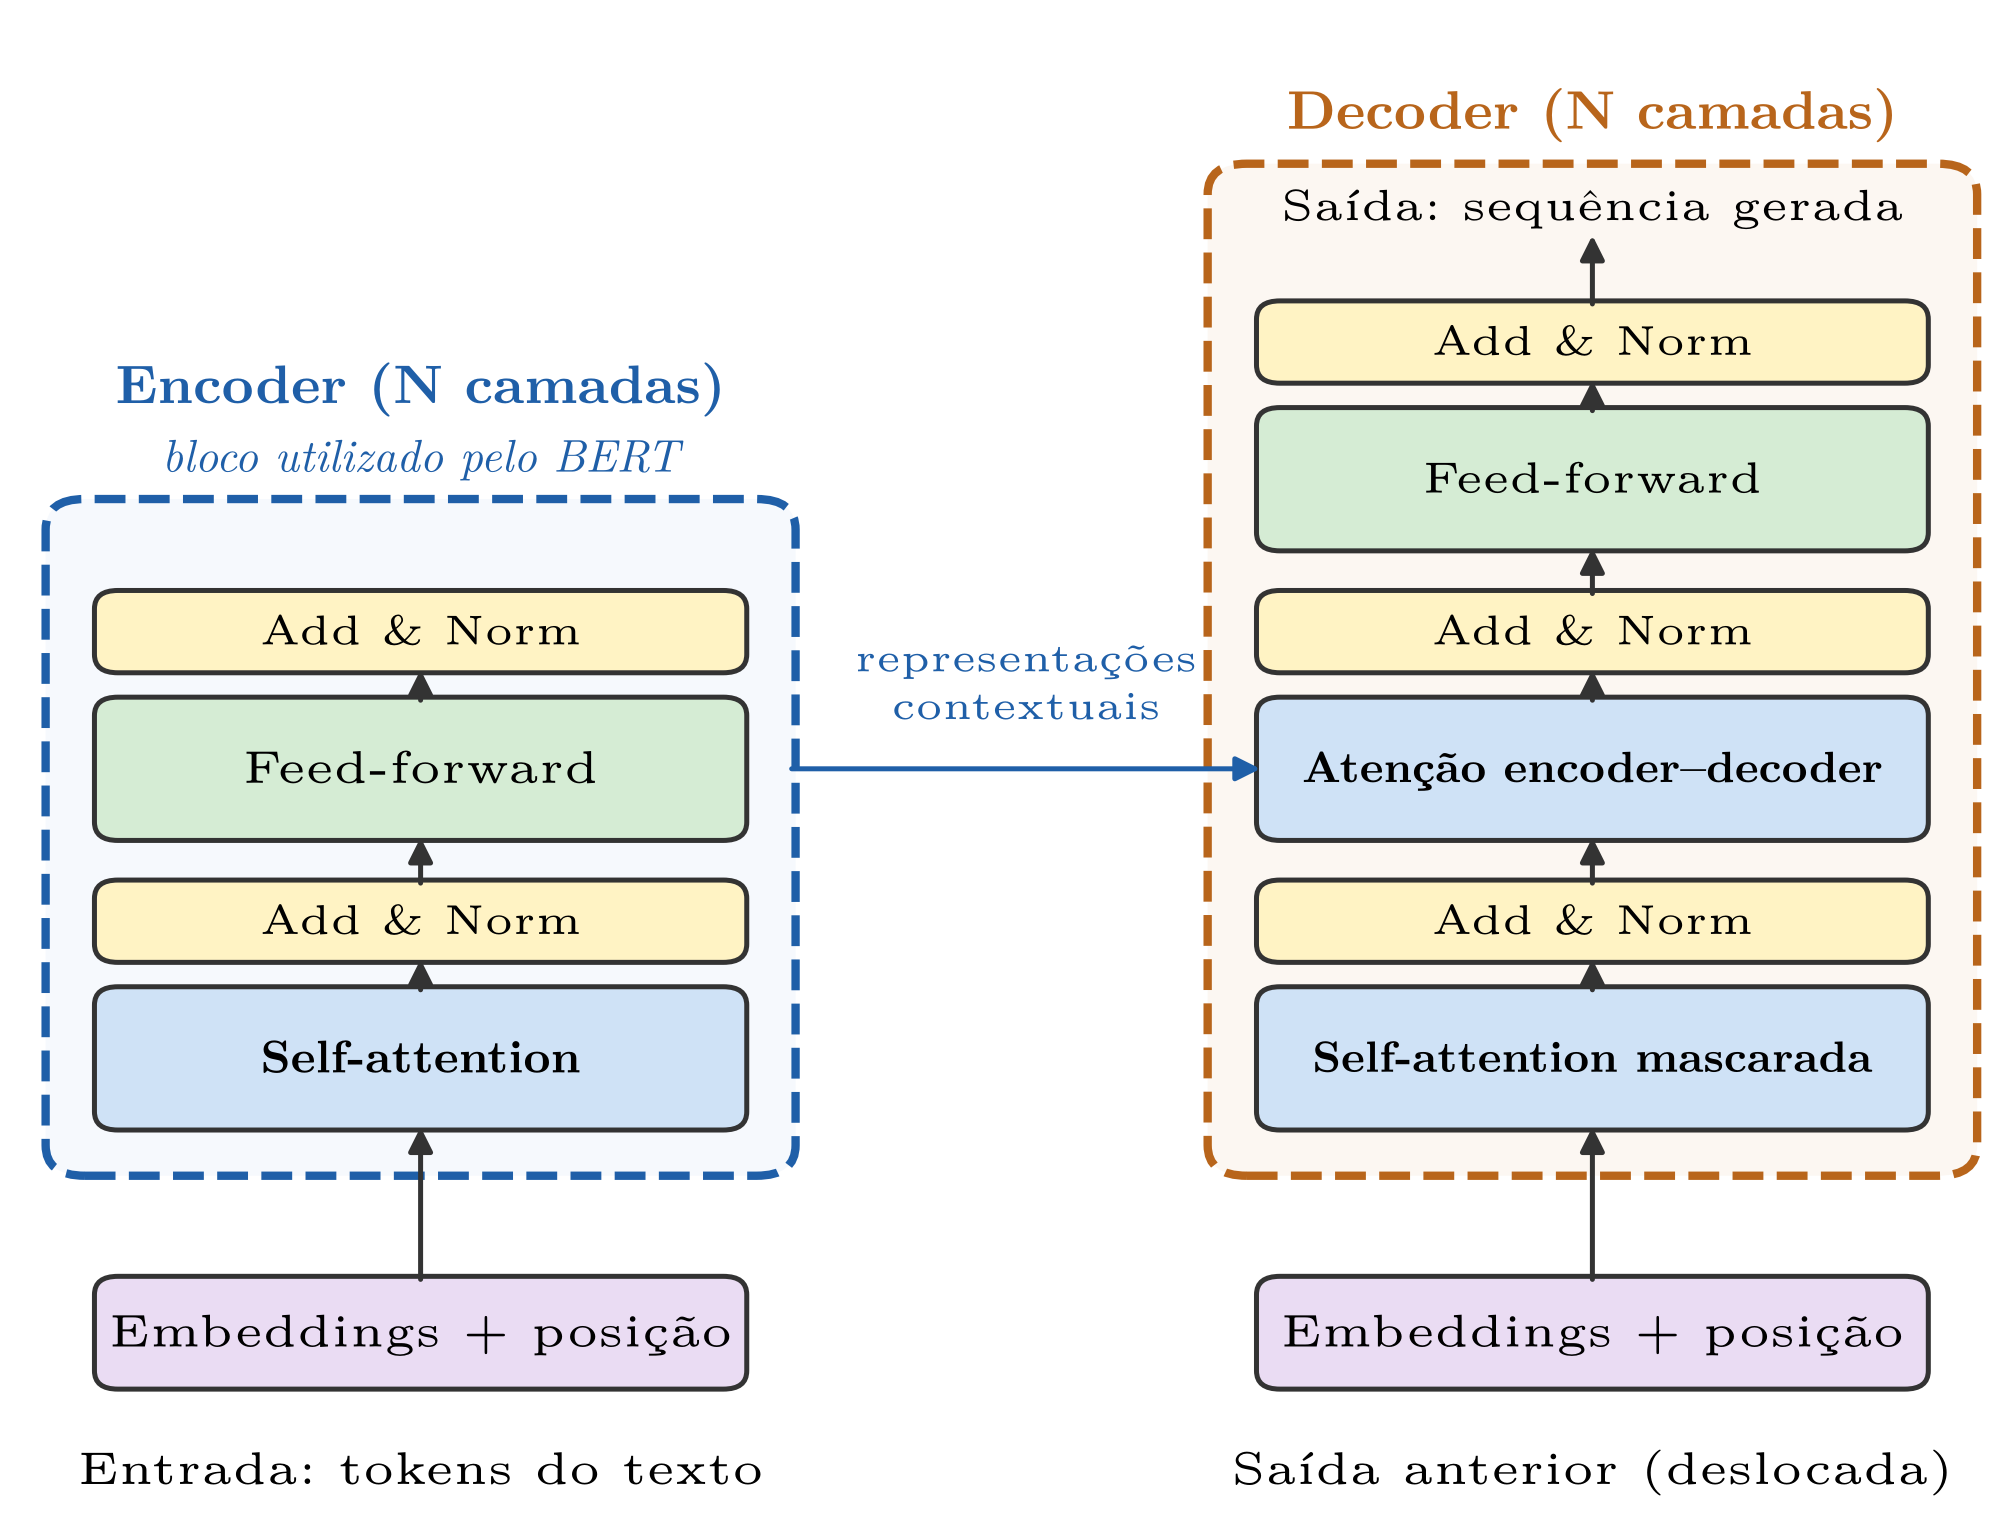
\includegraphics[width=0.85\textwidth]{imagens/transformer_arquitetura.png}
    \legend{Fonte: Elaborado pelos autores, com base em \citeonline{vaswani2017}}
\end{figure}

A arquitetura \textit{Transformer}, proposta por \citeonline{vaswani2017}, 
introduziu o mecanismo de \textit{self-attention} como alternativa às redes 
recorrentes para processamento de sequências. As RNN (\textit{Recurrent Neural Network} -- Rede Neural Recorrente) são uma classe de redes neurais 
projetadas para processar dados sequenciais, nos quais o contexto e a ordem 
temporal importam, processando os \textit{tokens} um por vez, da esquerda para 
a direita. As LSTM (\textit{Long Short-Term Memory} -- Memória de Longo e Curto Prazo) são um tipo especializado 
de RNN projetado para aprender dependências de longo prazo em sequências, 
mitigando o problema de desvanecimento do gradiente presente nas RNN simples. 
Apesar dessas melhorias, ambas as arquiteturas ainda processam a sequência de 
forma estritamente sequencial, o que limita o paralelismo computacional e 
dificulta a captura de relações entre termos distantes.

Para compreender o mecanismo de atenção, considere a frase ``o banco bloqueou 
meu acesso'': para determinar o significado da palavra ``banco'', é necessário 
considerar as demais palavras da frase — especialmente ``bloqueou'' e ``acesso'' 
— que indicam tratar-se de uma instituição financeira e não de um assento. O 
\textit{self-attention} formaliza esse processo: para cada \textit{token} da 
sequência, o mecanismo calcula um score de relevância em relação a todos os 
outros \textit{tokens}, indicando o quanto cada um deve ``influenciar'' a 
representação do \textit{token} atual. ``Atender simultaneamente a todas as 
posições'' significa que esse cálculo é realizado em paralelo para todos os 
pares de \textit{tokens} da sequência, possibilitando a captura de dependências 
de longo alcance de forma muito mais eficiente do que as arquiteturas recorrentes.

A Figura~\ref{fig:self_attention} ilustra esse cálculo para a palavra ``banco'': os pesos de atenção, que somam 1, indicam o quanto cada \textit{token} contribui para a nova representação de ``banco''. Nesse exemplo, ``acesso'' e ``bloqueou'' recebem os maiores pesos, o que leva o modelo a representar ``banco'' como instituição financeira.
 
\begin{figure}[H]
    \caption{Exemplo ilustrativo de \textit{self-attention} para o \textit{token} ``banco''}
    \label{fig:self_attention}
    \centering
    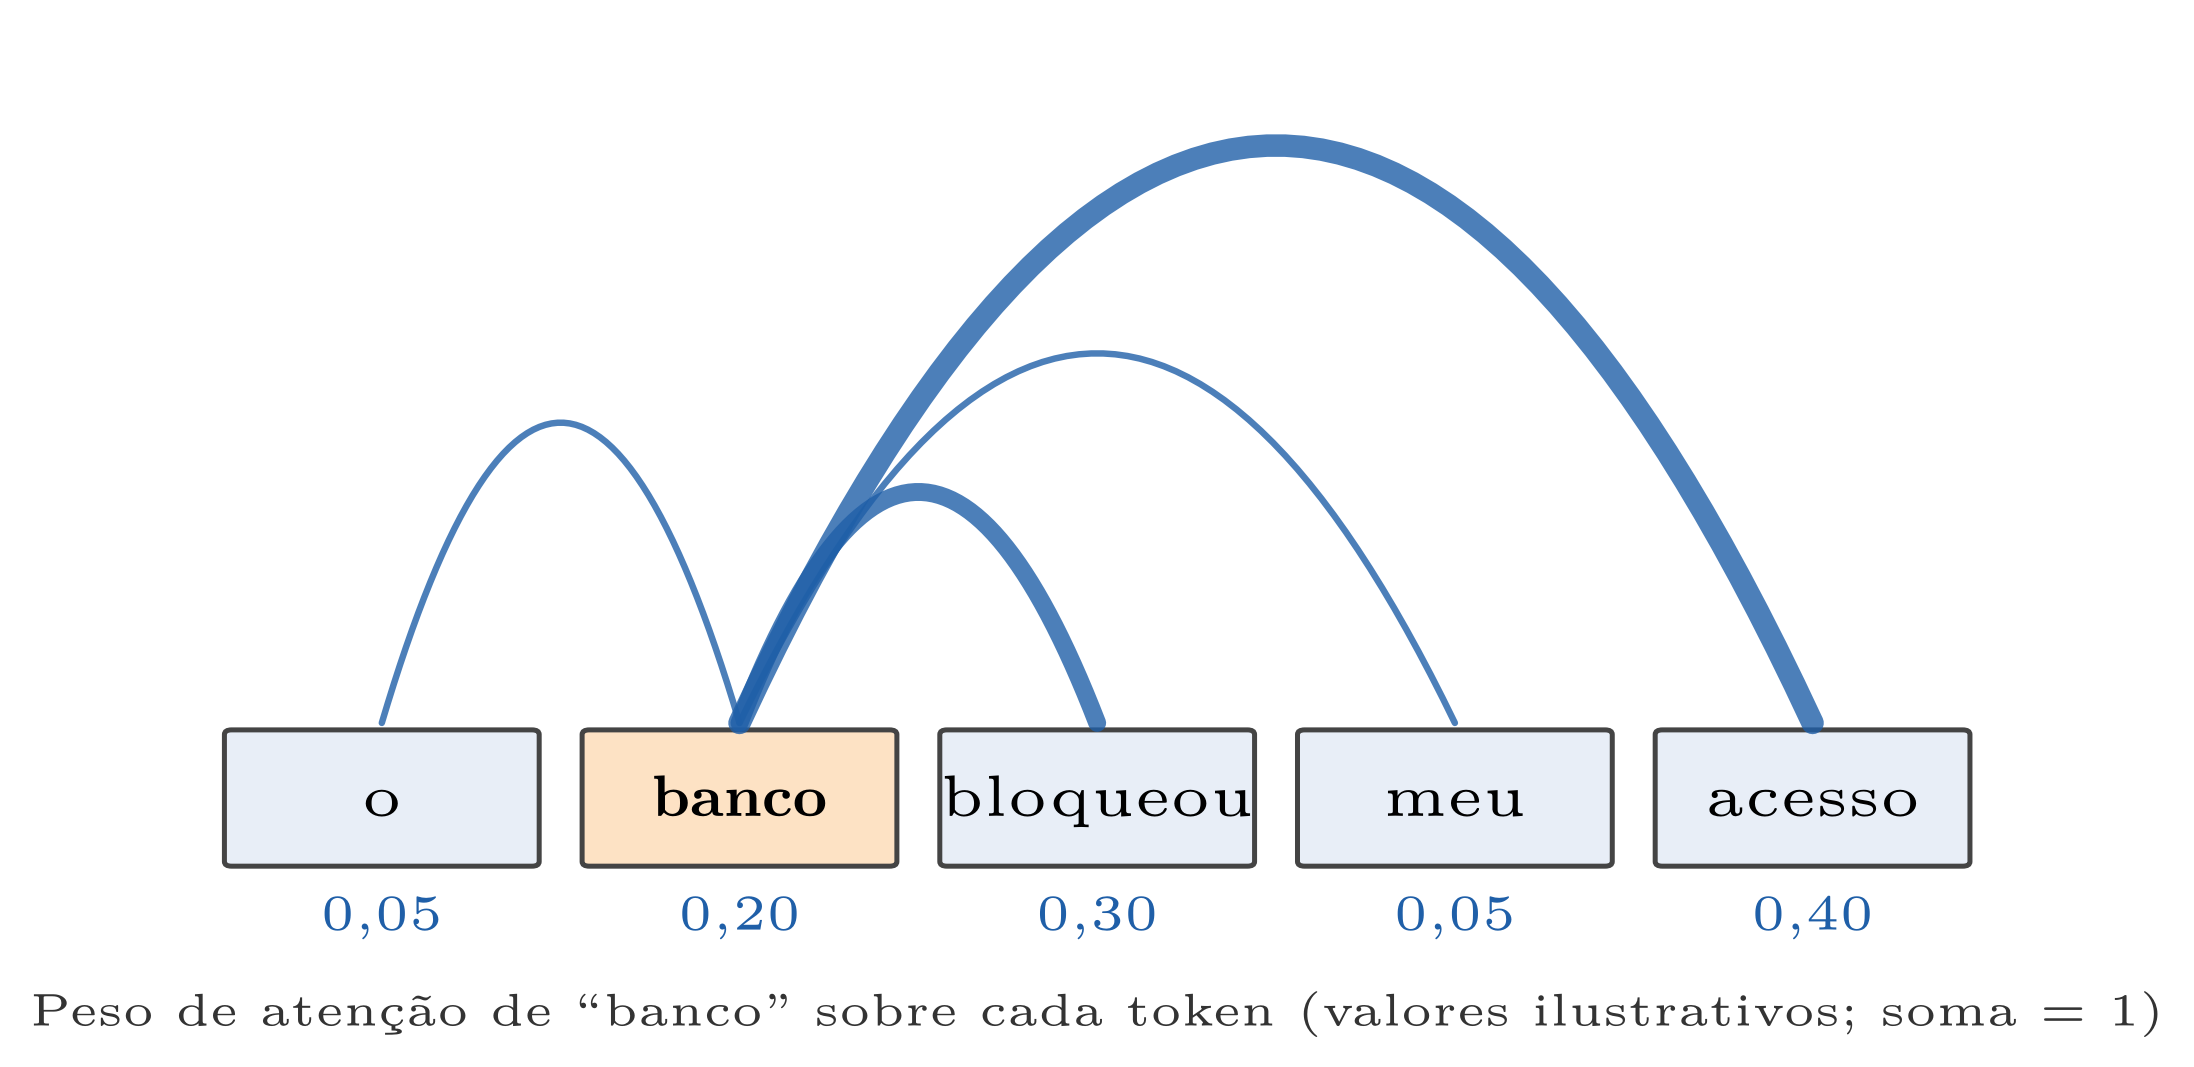
\includegraphics[width=0.85\textwidth]{imagens/self_attention.png}
    \legend{Fonte: Elaborado pelos autores (valores ilustrativos, não extraídos de um modelo treinado)}
\end{figure}

Modelos como o GPT utilizam atenção unidirecional (cada \textit{token} só pode 
atender aos \textit{tokens} anteriores). O BERT, por sua vez, utiliza atenção 
bidirecional: cada \textit{token} atende simultaneamente a todos os outros 
\textit{tokens} da sequência, tanto os que aparecem antes quanto os que aparecem 
depois. Essa bidirecionalidade é fundamental para a qualidade das representações 
contextualizadas geradas pelo modelo, uma vez que o significado de uma palavra 
frequentemente depende tanto de seu contexto anterior quanto posterior 
\cite{devlin2019}.

A Figura~\ref{fig:atencao_bidirecional} compara os dois tipos de atenção: na atenção unidirecional, cada \textit{token} só atende a si mesmo e aos anteriores; na bidirecional, atende a todos.
 
\begin{figure}[H]
    \caption{Atenção unidirecional e atenção bidirecional}
    \label{fig:atencao_bidirecional}
    \centering
    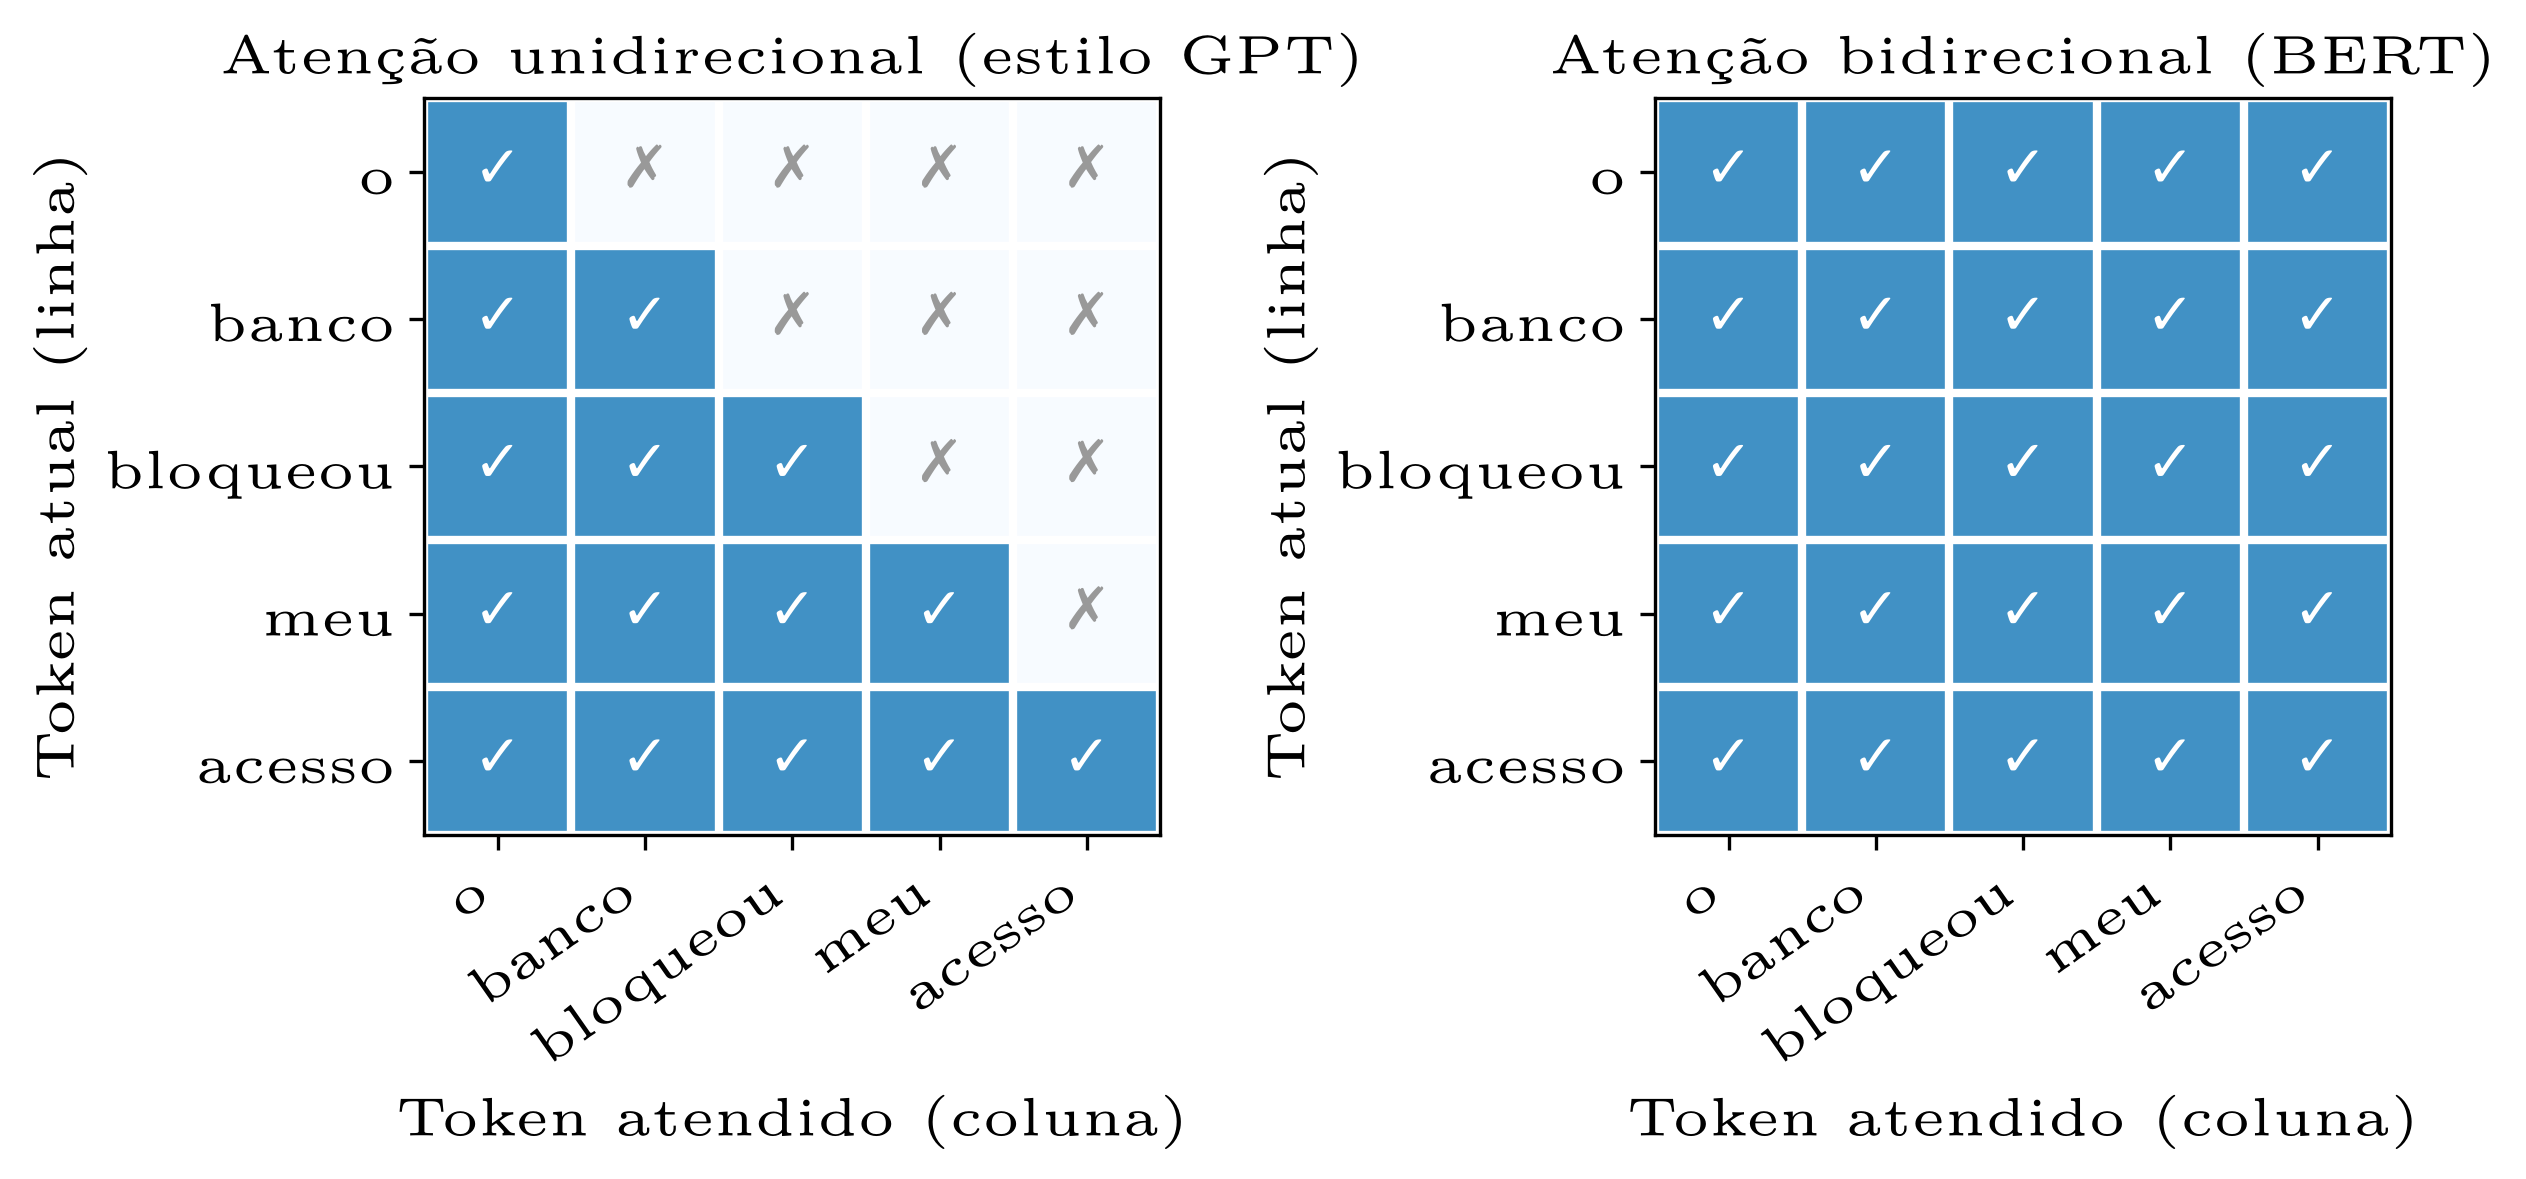
\includegraphics[width=0.9\textwidth]{imagens/atencao_bidirecional.png}
    \legend{Fonte: Elaborado pelos autores. Cada linha indica a quais \textit{tokens} a palavra daquela linha pode atender}
\end{figure}

% - - - - - - - - - - - - - - - - - - - - - - - - - - - - - - -
\subsubsection{Pré-treinamento — \textit{Masked Language Modeling} e \textit{Next Sentence Prediction}}
\label{subsubsec:bert_pretrain}

O BERT é pré-treinado em dois objetivos complementares sobre grandes corpora textuais não rotulados. O primeiro, MLM (\textit{Masked Language Modeling} -- Modelagem de Linguagem com Máscara), mascara aleatoriamente 15\% dos \textit{tokens} de cada sequência de entrada e treina o modelo para predizer os \textit{tokens} mascarados a partir do contexto bidirecional restante. Esse objetivo força o modelo a aprender representações ricas que capturam o significado de cada palavra em seu contexto completo \cite{devlin2019}.

O segundo objetivo, NSP (\textit{Next Sentence Prediction} -- Predição da Próxima Sentença), treina o modelo a determinar se duas sentenças apresentadas em sequência são consecutivas no texto original ou foram pareadas aleatoriamente. Esse objetivo permite ao modelo aprender relações semânticas entre sentenças, o que é útil para tarefas como inferência textual e resposta a perguntas.

% - - - - - - - - - - - - - - - - - - - - - - - - - - - - - - -
\subsubsection{\textit{Fine-tuning} para tarefas \textit{downstream}}
\label{subsubsec:bert_finetune}

Após o pré-treinamento, o BERT pode ser adaptado para tarefas específicas por meio do processo de \textit{fine-tuning}: o modelo pré-treinado é inicializado com os pesos aprendidos no pré-treinamento, uma camada de saída específica para a tarefa é adicionada ao topo da arquitetura, e o modelo completo é treinado por um número reduzido de épocas sobre o conjunto de dados rotulado da tarefa-alvo \cite{devlin2019}.

Essa abordagem de pré-treinamento seguido de \textit{fine-tuning} é particularmente eficaz porque o modelo já adquiriu conhecimento linguístico geral durante o pré-treinamento, e o \textit{fine-tuning} apenas adapta esse conhecimento para o domínio e a tarefa específicos. Para classificação de chamados de TI, o \textit{fine-tuning} ajusta os pesos do modelo para que as representações produzidas sejam especialmente discriminativas entre as categorias de chamados presentes no \textit{dataset}.

% ---------------------------------------------------------------
\subsection{BERT}
\label{subsec:bert_modelo}

% - - - - - - - - - - - - - - - - - - - - - - - - - - - - - - -
\subsubsection{Arquitetura e configurações \textit{BERT-base} e \textit{BERT-large}}
\label{subsubsec:bert_arquitetura}

\citeonline{devlin2019} propuseram o BERT em duas configurações. O \textit{BERT-base} possui 12 camadas de \textit{encoder} \textit{Transformer}, 12 cabeças de atenção e 110 milhões de parâmetros. O \textit{BERT-large} possui 24 camadas, 16 cabeças de atenção e 340 milhões de parâmetros. Ambas as versões foram pré-treinadas sobre o corpus da Wikipedia em inglês e o BookCorpus, totalizando aproximadamente 3,3 bilhões de palavras.

O BERT estabeleceu o estado da arte em onze tarefas de PLN no momento 
de sua publicação, incluindo classificação de texto, reconhecimento 
de entidades nomeadas, resposta a perguntas e inferência textual. 
Seu lançamento popularizou o uso de modelos pré-treinados em tarefas 
de PLN, consolidando a abordagem de pré-treinamento em larga escala 
seguido de \textit{fine-tuning} como a estratégia dominante para 
tarefas de PLN.

% - - - - - - - - - - - - - - - - - - - - - - - - - - - - - - -
\subsubsection{\textit{Token} [CLS] e classificação de sequências}
\label{subsubsec:bert_cls}

Para tarefas de classificação de sequências, o BERT utiliza um \textit{token} especial [CLS] (abreviação de \textit{Classification}, marcador inserido pelo modelo para agregar a representação global da sequência) inserido no início de cada sequência de entrada. Após o processamento pelas camadas de \textit{encoder}, a representação vetorial correspondente ao [CLS] agrega informação contextual de toda a sequência e é usada como entrada para a camada de classificação \cite{devlin2019}. Durante o \textit{fine-tuning}, essa camada de classificação, tipicamente uma camada \textit{linear} seguida de \textit{softmax}, aprende a mapear a representação do [CLS] para as probabilidades de cada categoria. 
Neste trabalho, essa representação é usada para classificar o chamado de TI em uma das categorias predefinidas, e os valores SHAP e LIME são calculados sobre os tokens de entrada para identificar quais contribuíram mais para a predição.


% ---------------------------------------------------------------
\subsection{BERTimbau — BERT para o português brasileiro}
\label{subsec:bertimbau}

% - - - - - - - - - - - - - - - - - - - - - - - - - - - - - - -
\subsubsection{Corpus de pré-treinamento e diferenças em relação ao mBERT}
\label{subsubsec:bertimbau_corpus}

\citeonline{souza2020} desenvolveram o BERTimbau, modelo BERT pré-treinado especificamente para o português brasileiro, a partir do BrWaC (\textit{Brazilian Web as Corpus}), um grande corpus de páginas \textit{web} em português com 2,68 bilhões de \textit{tokens}. Duas versões foram disponibilizadas: BERTimbau-base (12 camadas, 110M parâmetros) e BERTimbau-large (24 camadas, 335M parâmetros).

A principal diferença em relação ao mBERT está no foco linguístico: o mBERT foi pré-treinado sobre 104 idiomas simultaneamente, o que dilui a capacidade de representação para cada língua individualmente. O BERTimbau, ao ser pré-treinado exclusivamente sobre texto em português brasileiro, aprende padrões morfológicos, sintáticos e semânticos específicos do idioma com maior profundidade.

% - - - - - - - - - - - - - - - - - - - - - - - - - - - - - - -
\subsubsection{Desempenho em tarefas de PLN em PT-BR}
\label{subsubsec:bertimbau_desempenho}

\citeonline{souza2020} avaliaram o BERTimbau em três tarefas de PLN em português: reconhecimento de entidades nomeadas (NER), similaridade textual entre sentenças e inferência textual (\textit{Recognizing Textual Entailment}). O modelo obteve desempenho de estado da arte nas três tarefas, consolidando-se como referência para aplicações de PLN em PT-BR.

Para o presente trabalho, a escolha do BERTimbau em detrimento do mBERT é motivada por dois fatores. Primeiro, os chamados de suporte analisados estão em português brasileiro, idioma para o qual o BERTimbau possui representações mais ricas. Segundo, os chamados utilizam terminologia técnica de TI em português, que pode diferir substancialmente de sua versão em inglês. E o BERTimbau, pré-treinado em corpus nacional, tem maior probabilidade de ter encontrado esse vocabulário durante o pré-treinamento.

O BERTimbau foi mantido como modelo deste trabalho, dado que os chamados analisados estão predominantemente em português brasileiro. A avaliação de modelos multilíngues ou mais recentes fica indicada como trabalho futuro.

% ---------------------------------------------------------------
\subsection{\textit{Fine-tuning} de BERT para classificação de chamados de TI}
\label{subsec:bert_tickets}

A aplicação de BERT e modelos derivados à classificação de chamados de TI tem demonstrado resultados expressivos na literatura recente. \citeonline{borges2024} realizou uma comparação sistemática entre BERT e algoritmos clássicos, SVM e \textit{Naive Bayes}, em tarefas de classificação de texto em português e inglês, utilizando quatro \textit{datasets} públicos. Os resultados confirmaram que o BERT supera consistentemente os modelos tradicionais em acurácia e F1, especialmente em tarefas multiclasse com nuances semânticas mais complexas, embora com custo computacional consideravelmente maior.

\citeonline{zemp2021} comparou CNN, BiLSTM e RoBERTa sobre mais de um 
milhão de \textit{tickets} reais de um banco privado de médio porte, em 
mais de 300 classes. A melhor CNN atingiu F1-macro de 0,75. Com o 
\textit{fine-tuning} simples, o RoBERTa ficou abaixo desse valor; somente 
após um pré-treinamento adicional do modelo de linguagem com os próprios 
\textit{tickets} ele superou a CNN, por uma margem de 0,018.

\citeonline{razma2026} compararam regressão logística com TF-IDF 
frente a mBERT e XLM-RoBERTa, uma variante do RoBERTa desenvolvida 
especificamente para lidar com múltiplos idiomas simultaneamente, 
em um corpus de 87 mil \textit{tickets} multilíngues de uma empresa 
de manufatura. Os resultados confirmaram que \textit{transformers} 
superam modelos clássicos em macro-F1, especialmente para classes 
de baixa frequência e semanticamente complexas. Os autores aplicaram o LIME ao mBERT e à regressão logística, e o SHAP à regressão logística, o que mostra ser viável explicar um BERT \textit{fine-tuned} com LIME sobre chamados reais de ITSM; eles afirmam que as explicações contribuem para a interpretabilidade e a confiança.

% ---------------------------------------------------------------
\subsection{Definição e motivação}
\label{subsec:xai_definicao}

% - - - - - - - - - - - - - - - - - - - - - - - - - - - - - - -
\subsubsection{O problema da caixa-preta em aprendizado profundo}
\label{subsubsec:xai_caixapreta}

Modelos de aprendizado profundo, incluindo o BERT, são frequentemente descritos como caixas-pretas: produzem predições com alta acurácia, mas sem revelar quais características da entrada determinaram a saída. Isso acontece porque esses modelos possuem centenas de milhões de 
parâmetros internos, valores numéricos ajustados durante o 
treinamento, organizados em múltiplas camadas de cálculos complexos. 
Essa estrutura torna impossível para um ser humano acompanhar ou 
explicar, passo a passo, como o modelo chegou a uma determinada 
decisão \cite{salih2023}.

Em contextos como a triagem de chamados de TI, essa opacidade representa um problema prático concreto. Analistas de suporte e gestores precisam auditar as decisões do sistema, identificar erros sistemáticos e eventualmente contestar categorizações incorretas. Um modelo que não fornece justificativa para suas predições é difícil de depurar, difícil de melhorar e difícil de justificar perante \textit{stakeholders} (partes interessadas, como gestores e diretores) organizacionais.

% - - - - - - - - - - - - - - - - - - - - - - - - - - - - - - -
\subsubsection{Confiança, explicabilidade e adoção em produção}
\label{subsubsec:xai_confianca}

No estudo de \citeonline{zemp2021}, a equipe de suporte recusou parte do sistema de 
classificação, como discutido na Seção~\ref{subsubsec:helpdesk_caixapreta}. \citeonline{razma2026} afirmam 
que as explicações LIME favorecem a interpretabilidade e a confiança no sistema, 
pois permitem verificar se os termos destacados como mais influentes fazem sentido 
para aquela categoria específica, embora não tenham medido a reação dos operadores.

Essa ideia é consistente com a literatura de XAI mais ampla: as explicações
 ajudam os usuários a decidir se confiam em uma predição e a identificar modelos 
 que erram por razões inadequadas \cite{ribeiro2016}.


% - - - - - - - - - - - - - - - - - - - - - - - - - - - - - - -
\subsubsection{Taxonomia de métodos XAI — intrínsecos versus \textit{post-hoc}, locais versus globais}
\label{subsubsec:xai_taxonomia}

Os métodos de XAI podem ser classificados segundo duas dimensões principais \cite{salih2023}. A primeira dimensão distingue métodos intrínsecos dos métodos \textit{post-hoc}. Métodos intrínsecos são aqueles em que a interpretabilidade é uma propriedade do próprio modelo — árvores de decisão, regressão logística e modelos lineares em geral são interpretáveis por \textit{design}, pois seus parâmetros têm significado diretamente interpretável. Métodos \textit{post-hoc} são aplicados após o treinamento, sobre modelos de qualquer complexidade, e produzem explicações sem modificar o modelo original.

A segunda dimensão distingue explicações locais das globais. Explicações locais descrevem o comportamento do modelo para uma instância específica de entrada (exemplo: por que o modelo classificou \textit{este} chamado como ``Acesso''?). Explicações globais descrevem o comportamento geral do modelo (exemplo: quais termos são mais importantes para cada categoria em média?). SHAP e LIME são métodos \textit{post-hoc} que operam primariamente no nível local, embora o SHAP permita agregações que produzem explanações globais.

% ---------------------------------------------------------------
\subsection{LIME — \textit{Local Interpretable Model-Agnostic Explanations}}
\label{subsec:lime}

% - - - - - - - - - - - - - - - - - - - - - - - - - - - - - - -
\subsubsection{Funcionamento — perturbações e modelo local interpretável}
\label{subsubsec:lime_funcionamento}

LIME foi proposto por \citeonline{ribeiro2016} como um método de 
explicação local que funciona com qualquer tipo de modelo e qualquer 
tipo de entrada, sem precisar conhecer sua estrutura interna. O método 
parte do princípio de que, embora um modelo de aprendizado profundo 
seja globalmente complexo e não-linear, seu comportamento em torno 
de um exemplo específico pode ser aproximado por um modelo simples 
e interpretável.

O processo de geração de uma explicação LIME para uma instância de 
texto ocorre em quatro etapas. Primeiro, o texto original é perturbado 
pela remoção ou substituição aleatória de palavras, criando um conjunto 
de versões modificadas da frase. Segundo, cada versão modificada é 
submetida ao modelo para que ele produza uma predição, permitindo 
observar se e como a resposta muda conforme as palavras são alteradas. 
Terceiro, as versões modificadas são ponderadas pela similaridade com 
o texto original, sendo que versões mais próximas do original recebem 
peso maior. Quarto, um modelo linear simples é ajustado sobre esse 
conjunto, e seus coeficientes indicam quais palavras mais influenciaram 
a classificação \cite{ribeiro2016}.

Formalmente, o LIME resolve o seguinte problema de otimização 
para encontrar a explicação $\xi(x)$ de uma instância $x$:

\begin{equation}
\xi(x) = \arg\min_{g \in G} \mathcal{L}(f, g, \pi_x) + \Omega(g)
\end{equation}

onde $f$ é o modelo de caixa-preta a ser explicado, $G$ é o 
conjunto de modelos interpretáveis candidatos, $\mathcal{L}$ é 
uma função de perda que mede a fidelidade da explicação $g$ ao 
modelo $f$ na vizinhança de $x$, $\pi_x$ é uma função de 
proximidade que pondera as instâncias perturbadas pela 
similaridade com $x$, e $\Omega(g)$ é uma medida de 
complexidade do modelo explicativo \cite{ribeiro2016}. O 
objetivo é encontrar o modelo interpretável mais simples 
possível que seja localmente fiel ao comportamento do modelo 
complexo.

A Figura~\ref{fig:lime_exemplo} ilustra esse processo: as palavras 
destacadas indicam sua contribuição positiva ou negativa para a 
classe predita.

\begin{figure}[H]
    \caption{Exemplo de explicação gerada pelo LIME}
    \label{fig:lime_exemplo}
    \centering
    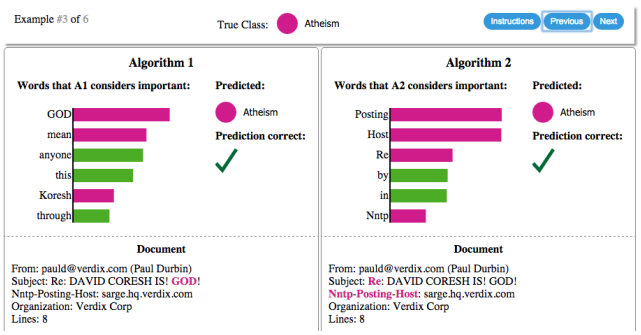
\includegraphics[width=0.75\textwidth]{imagens/lime_exemplo.png}
    \legend{Fonte: \citeonline{ribeiro2016}}
\end{figure}

% - - - - - - - - - - - - - - - - - - - - - - - - - - - - - - -
\subsubsection{Aplicação em classificação de texto}
\label{subsubsec:lime_texto}

No contexto de classificação de texto, cada palavra (ou \textit{token}) da entrada é tratada como uma \textit{feature}, ou seja, uma característica binária que indica se está presente ou ausente no texto. A explicação LIME indica quais palavras, quando presentes, aumentam a probabilidade de cada classe, e quais palavras a diminuem. O resultado pode ser visualizado como um destaque colorido sobre o texto original, onde palavras em verde contribuem positivamente para a classe predita e palavras em vermelho contribuem negativamente \cite{mustafa2025}.

\citeonline{mustafa2025} demonstraram que a aplicação de LIME na 
classificação de texto não apenas produz explicações úteis para o 
usuário final, mas também contribui para melhorar o processo de 
pré-processamento: ao revelar que \textit{stopwords}, palavras muito 
frequentes e de pouco conteúdo informativo, como artigos e preposições 
(``de'', ``o'', ``para''), recebem pesos desproporcionalmente altos 
nas explicações, o LIME evidenciou a necessidade de sua remoção.

% - - - - - - - - - - - - - - - - - - - - - - - - - - - - - - -
\subsubsection{Vantagens e limitações}
\label{subsubsec:lime_limitacoes}

A principal vantagem do LIME é sua generalidade: o método funciona com qualquer modelo e qualquer tipo de entrada sem necessidade de acesso ao interior do modelo. Isso o torna especialmente adequado para modelos de caixa-preta como o BERT, cujos mecanismos internos são de difícil interpretação direta.

Sua principal limitação é a instabilidade das explicações. Por 
depender de amostragem aleatória de perturbações, execuções diferentes 
do LIME sobre a mesma instância podem produzir explicações distintas, 
especialmente quando há colinearidade entre as \textit{features}, 
ou seja, quando algumas características extraídas do texto são muito 
parecidas ou carregam informações semelhantes \cite{salih2023}. Para 
mitigar essa instabilidade, recomenda-se executar o LIME múltiplas 
vezes e analisar a consistência das explicações, ou fixar a semente 
aleatória para garantir reprodutibilidade.

% ---------------------------------------------------------------
\subsection{SHAP — \textit{SHapley Additive exPlanations}}
\label{subsec:shap}

% - - - - - - - - - - - - - - - - - - - - - - - - - - - - - - -
\subsubsection{Fundamentos — valores de Shapley da teoria dos jogos}
\label{subsubsec:shap_fundamentos}

SHAP foi proposto por \citeonline{lundberg2017} com base nos valores 
de Shapley da teoria dos jogos cooperativos. O problema que o SHAP 
resolve é: dada uma predição específica de um modelo, como distribuir 
o ``crédito'' por essa predição de forma justa entre as 
\textit{features} de entrada?

Na teoria dos jogos, o valor de Shapley de um jogador em um jogo 
cooperativo é calculado como a média ponderada de quanto cada jogador 
contribuiu individualmente em todas as combinações possíveis com os 
demais jogadores. \citeonline{lundberg2017} adaptam esse conceito 
para o contexto de modelos de aprendizado de máquina: cada 
\textit{feature} é um ``jogador'', a predição do modelo é o 
``valor do jogo'', e o valor SHAP de cada \textit{feature} mede 
o quanto ela contribuiu para a predição, considerando todas as 
possíveis ordens em que as \textit{features} poderiam ser incluídas.

Formalmente, o valor de Shapley de uma \textit{feature} $i$ 
é calculado como:

\begin{equation}
\phi_i = \sum_{S \subseteq F \setminus \{i\}} 
\frac{|S|!(|F| - |S| - 1)!}{|F|!} 
\left[ f_{S \cup \{i\}}(x_{S \cup \{i\}}) - f_S(x_S) \right]
\end{equation}

onde $F$ é o conjunto de todas as \textit{features}, $S$ é um 
subconjunto que não inclui $i$, $f(S)$ é a predição do modelo 
usando apenas as \textit{features} em $S$, e 
$f(S \cup \{i\})$ é a predição incluindo a \textit{feature} 
$i$ \cite{lundberg2017}. O fator 
$\frac{|S|!(|F| - |S| - 1)!}{|F|!}$ garante que todas as 
ordenações possíveis de inclusão das \textit{features} sejam 
consideradas com peso igual, assegurando a propriedade de 
simetria.

A Figura~\ref{fig:shap_exemplo} ilustra esse conceito: cada 
\textit{feature} desloca a predição do valor base até o 
valor final do modelo.

\begin{figure}[H]
    \caption{Representação dos valores SHAP por \textit{feature}}
    \label{fig:shap_exemplo}
    \centering
    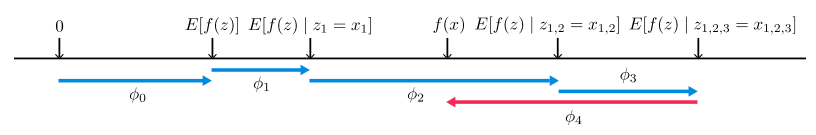
\includegraphics[width=0.75\textwidth]{imagens/shap_exemplo.png}
    \legend{Fonte: \citeonline{lundberg2017}}
\end{figure}

% - - - - - - - - - - - - - - - - - - - - - - - - - - - - - - -
\subsubsection{Propriedades matemáticas — eficiência, simetria e ausência}
\label{subsubsec:shap_propriedades}

A formulação baseada em valores de Shapley garante ao SHAP propriedades matemáticas desejáveis, que o distinguem de métodos \textit{ad hoc} de atribuição de importância. \citeonline{lundberg2017} as formulam como acurácia local, ausência (\textit{missingness}) e consistência. Na forma clássica dos axiomas de Shapley, as propriedades de interesse aqui são três. A propriedade de eficiência estabelece que a soma dos valores SHAP de todas as \textit{features} iguala a diferença entre a predição do modelo para a instância em questão e o valor base (predição média do modelo sobre o conjunto de dados). A propriedade de simetria estabelece que \textit{features} com contribuições iguais ao modelo recebem valores SHAP iguais, independentemente de sua posição na entrada. A propriedade de ausência estabelece que \textit{features} que não afetam a predição recebem valor SHAP zero.

Essas propriedades conferem ao SHAP uma fundamentação teórica sólida que o LIME não possui, tornando suas explicações mais consistentes e matematicamente justificáveis.

% - - - - - - - - - - - - - - - - - - - - - - - - - - - - - - -
\subsubsection{Cálculo do SHAP em modelos de texto}
\label{subsubsec:shap_kernel}

Calcular o valor exato de Shapley se torna inviável quando o modelo 
possui muitas \textit{features}, pois seria necessário testar todas 
as combinações possíveis entre elas, o que cresce exponencialmente. 
Para resolver isso, o \textit{KernelSHAP} \cite{lundberg2017} estima 
esses valores testando apenas uma amostra dessas combinações, tornando 
o método viável mesmo em modelos de texto, onde cada \textit{token} 
é tratado como uma \textit{feature}.

Neste trabalho, o SHAP foi calculado com a biblioteca \textit{shap}, tratando cada palavra distinta do campo como uma \textit{feature} e a probabilidade da classe predita como o valor a ser explicado. Nos campos com até 10 palavras distintas, o valor de Shapley foi calculado de forma exata, testando todas as combinações; acima disso, foi estimado por amostragem de permutações, e não pelo \textit{KernelSHAP}. O resultado é um valor por palavra: valores SHAP positivos contribuem para a classe predita e valores negativos contribuem contra ela. Esses valores são utilizados como pesos dos nós no grafo de co-ocorrência, em conjunto com os valores LIME, permitindo comparação visual entre os dois métodos de explicabilidade.

% ---------------------------------------------------------------
\subsection{Comparação entre SHAP e LIME}
\label{subsec:shap_lime}

% - - - - - - - - - - - - - - - - - - - - - - - - - - - - - - -
\subsubsection{Consistência e estabilidade das explicações}
\label{subsubsec:comparacao_consistencia}

\citeonline{salih2023} realizaram uma análise comparativa abrangente entre SHAP e LIME, avaliando suas propriedades teóricas e comportamento empírico em tarefas de classificação. Em termos de consistência, o SHAP demonstra maior estabilidade: por ser baseado em uma formulação matemática única com garantias teóricas, suas explicações são menos sensíveis à aleatoriedade do processo de amostragem. O LIME, por depender de perturbações aleatórias e de um processo de ajuste local, pode produzir explicações distintas para a mesma instância em execuções diferentes.

Os autores concluem que SHAP é preferível quando a consistência e a fundamentação teórica das explicações são prioritárias, enquanto o LIME pode ser preferível quando a velocidade de geração das explicações é mais importante do que a estabilidade.

% - - - - - - - - - - - - - - - - - - - - - - - - - - - - - - -
\subsubsection{Custo computacional}
\label{subsubsec:comparacao_custo}

Em termos de custo computacional, o LIME é mais eficiente que o 
\textit{KernelSHAP} em textos longos porque trabalha com um número 
fixo de perturbações. Já o \textit{KernelSHAP} exige uma amostragem 
muito maior de combinações de \textit{features} para gerar estimativas 
precisas, o que eleva o tempo de processamento \cite{salih2023}. 
Para textos curtos, como os chamados de suporte de TI, que tipicamente 
contêm poucas dezenas de palavras, essa diferença de custo é menos 
pronunciada.
% - - - - - - - - - - - - - - - - - - - - - - - - - - - - - - -
\subsubsection{Justificativa para uso conjunto neste trabalho}
\label{subsubsec:comparacao_justificativa}

A decisão de implementar e comparar SHAP e LIME neste trabalho, em vez de escolher apenas um dos métodos, é fundamentada em duas razões. Primeiro, a comparação entre os dois métodos produz evidência empírica sobre a qualidade e consistência das explicações geradas para chamados de TI em PT-BR, contribuição metodológica relevante para a literatura sobre XAI em domínios especializados. Segundo, a construção do grafo de co-ocorrência proposto utiliza os 
valores SHAP e LIME como pesos dos nós, permitindo avaliar 
se a escolha do método de XAI afeta a estrutura do grafo resultante.

% ---------------------------------------------------------------
\subsection{XAI aplicado a classificação de texto e tickets de TI}
\label{subsec:xai_aplicado}

% - - - - - - - - - - - - - - - - - - - - - - - - - - - - - - -
\subsubsection{LIME em classificação multiclasse de texto}
\label{subsubsec:xai_mustafa}

\citeonline{mustafa2025} propuseram um \textit{framework} de 
classificação de texto que combina PLN e XAI. O sistema inclui 
pré-processamento com NLTK (\textit{Natural Language Toolkit} -- Kit de Ferramentas de Linguagem Natural), 
balanceamento de classes com SMOTE (\textit{Synthetic Minority Oversampling Technique} -- Técnica de Sobreamostragem Sintética de Minorias), 
técnica que cria exemplos sintéticos das classes minoritárias a partir da interpolação 
entre exemplos vizinhos, para lidar com \textit{datasets} desbalanceados, 
e validação cruzada estratificada repetida: uma técnica que divide 
os dados em múltiplos subconjuntos para avaliar o modelo de forma 
mais robusta, garantindo que todas as classes estejam representadas 
em cada divisão. O modelo utilizado foi um híbrido de regressão 
\textit{ridge} com regressão logística. O LIME foi utilizado para 
validar a explicabilidade das classificações em seis domínios 
distintos: medicina, esportes, entretenimento, política, tecnologia 
e negócios. O modelo híbrido atingiu 99\% de acurácia após a 
aplicação do pré-processamento informado pelas explanações LIME.

O trabalho demonstra que a integração de XAI ao \textit{pipeline} 
de classificação não é apenas uma camada de interpretabilidade 
adicionada ao final do processo, mas pode também influenciar 
decisões de pré-processamento e seleção de \textit{features}, 
melhorando a qualidade do modelo como um todo.

% - - - - - - - - - - - - - - - - - - - - - - - - - - - - - - -
\subsubsection{SHAP e LIME em ambiente ITSM corporativo}
\label{subsubsec:xai_razma}

\citeonline{razma2026} aplicaram o LIME à regressão logística com \textit{TF-IDF} e ao mBERT \textit{fine-tuned}, e o SHAP à regressão logística, em um ambiente ITSM corporativo real. Os resultados qualitativos das explicações foram significativamente distintos: o modelo linear tendia a destacar palavras-chave literais com alta frequência no corpus, enquanto o BERT destacava termos semanticamente coerentes com o significado do chamado.

Essa diferença qualitativa nas explicações, documentada por 
\citeonline{razma2026}, sugere que o BERTimbau, combinado com SHAP 
e LIME, tende a produzir explicações mais acuradas em termos de 
importância de \textit{features} e potencialmente mais interpretáveis 
para analistas de TI sem formação em aprendizado de máquina, hipótese que este trabalho verifica empiricamente, 
avaliando se os termos destacados fazem sentido para cada categoria 
de chamado classificada.

% ---------------------------------------------------------------
\subsection{Fundamentos de grafos aplicados a texto}
\label{subsec:grafos_fundamentos}

% - - - - - - - - - - - - - - - - - - - - - - - - - - - - - - -
\subsubsection{Definição de grafo de co-ocorrência — nós, arestas e janela deslizante}
\label{subsubsec:grafos_definicao}

Um grafo de co-ocorrência de texto é uma estrutura 
$G = (V, E, W, f_{\text{shap}}, f_{\text{lime}})$, onde:

\begin{itemize}
    \item $V$ representa o conjunto de nós, correspondendo aos 
    \textit{tokens} únicos do texto;
    
    \item $E$ representa o conjunto de arestas, conectando pares 
    de \textit{tokens} que co-ocorrem dentro de uma janela 
    deslizante de tamanho $w$;
    
    \item $W$ representa os pesos das arestas, determinados pela 
    frequência de co-ocorrência entre os \textit{tokens};
    
    \item $f_{\text{shap}}$ representa os pesos dos nós calculados 
    pelo método SHAP, indicando a contribuição de cada 
    \textit{token} para a predição do modelo \cite{lundberg2017};
    
    \item $f_{\text{lime}}$ representa os pesos dos nós calculados 
    pelo método LIME, permitindo comparação visual entre os dois 
    métodos de explicabilidade \cite{ribeiro2016}.
\end{itemize}

A janela deslizante percorre o texto posição por posição; em cada 
posição, todos os pares de \textit{tokens} dentro da janela 
recebem uma aresta ou têm o peso de sua aresta existente 
incrementado \cite{yao2019}. Essa representação captura informação 
estrutural sobre o texto que as representações vetoriais não 
preservam: dois \textit{tokens} que frequentemente aparecem juntos 
no mesmo contexto estarão conectados por uma aresta de alto peso 
no grafo, independentemente de sua posição absoluta na sequência. 
Para chamados de TI, isso significa que termos técnicos que tendem 
a co-ocorrer em chamados de uma mesma categoria, como ``VPN'' e 
``acesso'' em chamados de conectividade, estarão estruturalmente 
próximos no grafo, com pesos de nós proporcionais à sua 
importância explicativa calculada por SHAP e LIME.
% - - - - - - - - - - - - - - - - - - - - - - - - - - - - - - -
\subsubsection{Ponderação de arestas — frequência, PMI}
\label{subsubsec:grafos_ponderacao}

O peso das arestas em um grafo de co-ocorrência pode ser determinado por diferentes métricas. A abordagem mais simples utiliza a frequência bruta de co-ocorrência, ou seja, a contagem de quantas vezes o par de \textit{tokens} co-ocorreu dentro da janela deslizante. Métricas mais sofisticadas, como a PMI (\textit{Pointwise Mutual Information} -- Informação Mútua Pontual), normalizam a frequência de co-ocorrência pelas frequências individuais de cada \textit{token}, favorecendo pares que co-ocorrem mais do que seria esperado pelo acaso \cite{yao2019}.

A PMI de um par de \textit{tokens} $a$ e $b$ é
\begin{equation}
\text{PMI}(a,b) = \log\frac{p(a,b)}{p(a)\,p(b)}
\end{equation}
onde $p(a,b)$ é a fração de janelas em que $a$ e $b$ aparecem juntos, e $p(a)$ e $p(b)$ são as frações de janelas em que cada um aparece. A frequência de co-ocorrência é, portanto, normalizada pelas frequências individuais dos \textit{tokens}: um par só recebe PMI alta se aparecer junto mais do que o esperado se os termos fossem independentes.

No presente trabalho, os pesos das arestas foram determinados pelo número de co-ocorrências do par dentro da janela deslizante (frequência bruta, sem normalização), enquanto os pesos dos \textit{nós}, que constituem o elemento central da proposta, foram determinados pelos valores SHAP e LIME de cada \textit{token}, calculados sobre as predições do BERTimbau, o que permite comparar visualmente a importância atribuída por cada método. Essa distinção entre ponderação de arestas (estrutura relacional) e ponderação de nós (relevância explicativa) é o diferencial da camada de visualização proposta.

% ---------------------------------------------------------------
\subsection{\textit{TextGCN} — formalização do grafo de co-ocorrência}
\label{subsec:textgcn}

% - - - - - - - - - - - - - - - - - - - - - - - - - - - - - - -
\subsubsection{Grafo heterogêneo documento-palavra}
\label{subsubsec:textgcn_grafo}

\citeonline{yao2019} propuseram o \textit{TextGCN} (\textit{Text Graph Convolutional Network}), modelo que constrói um único grafo heterogêneo para todo o corpus, conectando documentos e palavras. As arestas documento-palavra recebem pesos baseados em TF-IDF, refletindo a importância de cada palavra para cada documento. As arestas palavra-palavra recebem pesos baseados em PMI calculada sobre co-ocorrências em janela deslizante de tamanho 20 sobre todo o corpus, refletindo a força de associação semântica entre pares de palavras.

Essa estrutura permite que as GCN (\textit{Graph Convolutional Network} -- Rede Neural Convolucional em Grafos) propaguem informação simultaneamente entre documentos e palavras, capturando relações semânticas globais que modelos baseados em sequências não conseguem representar diretamente.

% - - - - - - - - - - - - - - - - - - - - - - - - - - - - - - -
\subsubsection{Redes neurais de grafos e propagação de informação}
\label{subsubsec:textgcn_gcn}

As GNN (\textit{Graph Neural Network} -- Rede Neural de Grafos) operam sobre grafos propagando informação entre nós vizinhos por meio de operações de agregação e transformação. Em cada camada da rede, a representação de cada nó é atualizada com base nas representações de seus vizinhos na iteração anterior \cite{yao2019}. Após múltiplas camadas, cada nó possui uma representação que agrega informação de sua vizinhança local de múltiplos saltos.

No contexto deste trabalho, a relevância do \textit{TextGCN} é fundamentalmente teórica: ele formaliza matematicamente a estrutura do grafo de co-ocorrência e demonstra sua utilidade para classificação de texto. O presente trabalho não implementou GCN: o grafo de co-ocorrência foi utilizado exclusivamente como estrutura de visualização das explicações XAI, e não como componente do modelo de classificação.

% ---------------------------------------------------------------
\subsection{Combinação de BERT com grafos de co-ocorrência}
\label{subsec:bert_grafo}

% - - - - - - - - - - - - - - - - - - - - - - - - - - - - - - -
\subsubsection{\textit{Embeddings} BERT como \textit{features} iniciais dos nós}
\label{subsubsec:bert_grafo_embeddings}

\citeonline{yang2021} propuseram o BEGNN (\textit{BERT-Enhanced Graph Neural Network} -- Rede Neural de Grafos Aprimorada por BERT), que combina representações contextualizadas do BERT com grafos de co-ocorrência para classificação de texto. Na arquitetura BEGNN, o BERT gera \textit{embeddings} contextualizados para cada \textit{token} da entrada; esses \textit{embeddings} são utilizados como \textit{features} iniciais dos nós do grafo de co-ocorrência correspondente ao documento. Em seguida, uma GCN propaga informação entre nós vizinhos, produzindo representações enriquecidas pela estrutura do grafo. A representação final do documento é obtida por agregação das representações dos nós.

Essa combinação aborda uma limitação do BERT quando utilizado isoladamente: o mecanismo de atenção do BERT captura relações entre \textit{tokens}, mas essas relações são implícitas nos pesos de atenção e não explicitamente estruturadas como um grafo. O grafo de co-ocorrência fornece uma estrutura explícita que complementa as representações contextualizadas.

% - - - - - - - - - - - - - - - - - - - - - - - - - - - - - - -
\subsubsection{Resultados em vocabulário técnico especializado}
\label{subsubsec:bert_grafo_resultados}

\citeonline{yang2021} avaliaram o BEGNN em múltiplos \textit{datasets} de classificação de texto, demonstrando que a combinação BERT + grafo supera tanto o BERT isolado quanto o \textit{TextGCN}, especialmente em \textit{datasets} com vocabulário técnico especializado. Esse resultado é relevante para o presente trabalho porque chamados de suporte de TI são exatamente o tipo de texto com vocabulário técnico especializado para o qual o BEGNN demonstrou vantagem, sugerindo que a estrutura de grafo de co-ocorrência captura informação complementar às representações do BERTimbau.

% ---------------------------------------------------------------
\subsection{Grafo de co-ocorrência combinado com XAI}
\label{subsec:grafo_xai}

% - - - - - - - - - - - - - - - - - - - - - - - - - - - - - - -
\subsubsection{Ponderação de nós por \textit{scores} de explicabilidade}
\label{subsubsec:grafo_xai_ponderacao}

\citeonline{talebi2025} apresentam o trabalho de maior proximidade 
metodológica com o presente TCC: aplicam RoBERTa combinado com LIME 
e um grafo de co-ocorrência para detectar \textit{body shaming}, 
prática de humilhar pessoas com base em sua aparência física, em 
redes sociais em inglês. No trabalho de \citeonline{talebi2025}, o grafo 
de co-ocorrência é construído com nós representando \textit{tokens} 
e arestas ponderadas pelos \textit{scores} LIME de cada \textit{token}. 
Os \textit{tokens} com maior importância LIME produzem arestas de 
maior peso com seus vizinhos na janela de co-ocorrência.

O presente trabalho adotou uma abordagem estruturalmente análoga, mas com diferenças importantes: utilizou o BERTimbau em vez do RoBERTa, aplicou os valores SHAP e LIME como pesos dos nós, em vez dos \textit{scores} LIME como pesos de arestas, e o domínio de aplicação foi a classificação de chamados de suporte de TI em português brasileiro. A escolha de ponderar os nós em vez das arestas reflete a intenção de destacar visualmente os \textit{tokens} individualmente mais relevantes para a predição, enquanto as arestas mantêm sua função de representar a estrutura de co-ocorrência do texto.

% - - - - - - - - - - - - - - - - - - - - - - - - - - - - - - -
\subsubsection{Visualização interativa como camada de auditabilidade}
\label{subsubsec:grafo_xai_visualizacao}

A literatura aponta que a combinação de grafos de co-ocorrência com \textit{scores} de explicabilidade pode ser exibida em interfaces interativas 
que tornam o processo decisório auditável. Nessa abordagem, os nós 
do grafo são dimensionados proporcionalmente à importância de cada 
\textit{token} calculada pelo método XAI, e as arestas são ponderadas 
pela frequência de co-ocorrência, produzindo uma representação visual 
que combina estrutura relacional do texto com relevância explicativa 
do modelo \cite{talebi2025}.

Essa camada de visualização tem o potencial de transformar a saída 
opaca do modelo em uma representação auditável, o que responde à 
limitação apontada por \citeonline{zemp2021} e \citeonline{razma2026}: 
sem acesso às razões da decisão, analistas de suporte não conseguem 
verificar o comportamento do modelo. O presente trabalho avalia a 
propriedade técnica de auditabilidade da representação proposta, sem 
medir a adoção efetiva do sistema por usuários. A solução proposta 
adota essa abordagem, cuja implementação é detalhada no 
Capítulo~\ref{cap:desenvolvimento}.
% ---------------------------------------------------------------
% 2.4 TRABALHOS CORRELATOS E LIMITAÇÕES
% ---------------------------------------------------------------
\section{Trabalhos correlatos e limitações}
\label{sec:trabalhos_relacionados}

Os quatro trabalhos a seguir enfrentaram o desafio de automatizar a triagem de chamados de suporte, servindo de base comparativa para a evolução proposta neste TCC.

\subsection{Trabalho 1: Text Classification of Service Desk Tickets}

\citeonline{zemp2021} abordou o problema da triagem automática num ambiente corporativo com mais de um milhão de chamados. 
Para resolvê-lo, o autor comparou modelos CNN, BiLSTM e RoBERTa. A metodologia envolveu o treino em larga escala 
num \textit{dataset} real de um banco privado de médio porte. Os resultados mostraram uma acurácia de 92\%. 
No entanto, a classificação automática entre incidentes e requisições foi considerada potencialmente 
perigosa pela equipe de suporte, devido ao risco de avaliações superficiais dos chamados. O presente trabalho 
diferencia-se por focar na explicabilidade via SHAP, LIME e grafos, permitindo que os analistas de TI 
entendam o ``porquê'' da classificação.

\subsection{Trabalho 2: A Hybrid Continual Machine Learning Model for Efficient Hierarchical Classification of Domain-Specific Text in The Presence of Class Overlap (Case Study: IT Support Tickets)}

\citeonline{wahba2023} enfrentou o mesmo desafio de classificação de \textit{tickets}, 
mas propôs uma abordagem focada em eficiência para domínios especializados. 
A solução utilizou um modelo híbrido (HOOM) que combina SVM linear e regras 
definidas com especialistas a um classificador \textit{online}. A metodologia 
demonstrou que em textos técnicos, modelos mais simples podem ser competitivos: 
a autora testou BERT e XLM e não encontrou ganho significativo sobre o SVM linear. 
Os resultados mostraram boa performance com baixo custo computacional. A limitação, 
em relação a este trabalho, é que a tese usa dados em inglês, não públicos, e não 
avalia explicações por palavra com métodos como SHAP e LIME. O presente trabalho 
adotou o BERTimbau, específico para PT-BR, que captura o contexto das palavras, 
e o combinou com SHAP, LIME e visualização em grafos para explicar as classificações.

\subsection{Trabalho 3: Classificação hierárquica de textos aplicado ao contexto chamados de suporte}

\citeonline{yokota2025} investigou a classificação de chamados de atendimento ao cliente especificamente em português brasileiro, utilizando \textit{Naive Bayes} e MLP sobre \textit{embeddings} do Multilingual E5. A metodologia focou na estrutura hierárquica das categorias (31 categorias e 240 subcategorias). Os resultados apresentaram F1-macro limitado, no máximo 61\%. A lacuna principal foi o desempenho baixo dos classificadores, que a autora associa ao desbalanceamento, à proximidade semântica entre categorias e ao vocabulário especializado, sem tratar da explicabilidade das decisões. O presente trabalho diferencia-se pelo ajuste fino de uma arquitetura de estado da arte (BERTimbau) pré-treinada em português e pela explicação das decisões com SHAP, LIME e grafos.

\subsection{Trabalho 4: AI-Based Classification of IT Support Requests in Enterprise Service Management Systems}

\citeonline{razma2026} compararam regressão logística com TF-IDF, mBERT e XLM-RoBERTa na classificação de mais de 87 mil chamados multilíngues de uma empresa de manufatura, e aplicaram o LIME (à regressão logística e ao mBERT) e o SHAP (à regressão logística) a exemplos de chamados. Os \textit{transformers} tiveram F1-macro maior, e as explicações do BERT destacaram termos mais contextuais que as do modelo linear. Pelo que o artigo apresenta, as explicações são mostradas em exemplos, sem medidas de fidelidade, estabilidade ou concordância entre os métodos, e sem estruturá-las em grafo. O presente trabalho mede essas propriedades para SHAP e LIME sobre o BERTimbau, em chamados em português, e as representa em um grafo de co-ocorrência.

\vspace{0.5cm}

\begin{table}[htb]
    \centering
    \caption{Comparação entre trabalhos relacionados}
    \label{tab:trabalhos_relacionados}
    \resizebox{\textwidth}{!}{
    \begin{tabular}{l|c|c|c|c|c}
        \toprule
        \textbf{Critério} & \textbf{Zemp (2021)} & \textbf{Wahba (2023)} & 
        \textbf{Yokota (2025)} & \textbf{Razma e Jurkus (2026)} & \textbf{Este trabalho} \\
        \midrule
        Objetivo & Classificação & Eficiência & Classificação PT-BR & 
        Classificação + XAI & Classificação + XAI \\
        \midrule
        Tecnologia & RoBERTa / CNN & SVM / HOOM & E5 + \textit{Naive Bayes} / MLP & 
        mBERT / XLM-R / Reg. logística & BERTimbau + Grafos \\
        \midrule
        Explicabilidade & Não & Intrínseca & Não aborda & LIME / SHAP (em exemplos) & SHAP / LIME / Grafos \\
        \midrule
        Limitação & Caixa-Preta & Dados em inglês, privados & Baixa Performance & 
        Sem medidas de qualidade das explicações & Custo Computacional \\
        \bottomrule
    \end{tabular}
    }
    \vspace{0.2cm}
    \legend{Fonte: Elaborado pelos autores}
\end{table}

% ---------------------------------------------------------------
\subsection{Limitações dos modelos existentes}
\label{subsec:helpdesk_limitacoes}

% - - - - - - - - - - - - - - - - - - - - - - - - - - - - - - -
\subsubsection{O debate BERT versus SVM em domínios especializados}
\label{subsubsec:helpdesk_debate}

\citeonline{wahba2023}, em sua tese de doutorado na Universidade de Western Ontario, propõe um contraponto relevante ao uso indiscriminado de modelos baseados em \textit{transformers} para classificação de texto em domínios especializados. Com base em quatro anos de estudos empíricos com dados reais de uma empresa parceira, a autora demonstra 
que chamados de suporte de TI utilizam vocabulário técnico específico 
e de baixa ambiguidade. Nesse contexto, a principal vantagem do BERT, que é compreender 
palavras com múltiplos sentidos dependendo do contexto, tem impacto 
reduzido, tornando o SVM com TF-IDF competitivo em termos de 
desempenho.

Com base nessa observação, \citeonline{wahba2023} propõe o modelo HOOM (\textit{Hybrid Online Offline Model} -- Modelo Híbrido \textit{Online} e \textit{Offline}), que combina um classificador SVM linear treinado em modo \textit{offline} com um classificador \textit{Passive Aggressive Classifier}. Esse segundo classificador 
é um algoritmo de aprendizado incremental que atualiza o modelo a cada nova amostra, mantendo-se ``passivo'' quando a predição está correta e ``agressivo'' ao corrigir erros e treinado em modo 
\textit{online} para detectar mudanças na distribuição dos dados ao longo do tempo. O modelo é descrito como mais eficiente, interpretável e reproduzível 
do que abordagens baseadas em \textit{transformers}, que são modelos 
de linguagem baseados em redes neurais profundas e que serão 
detalhados na Seção~\ref{subsec:bert_transformer}.

Este argumento é diretamente relevante para o presente trabalho, pois os cenários A (SVM com TF-IDF) e B (BERTimbau) permitem medir, nos chamados analisados, o ganho do modelo mais complexo (Seção~\ref{subsec:experimentos}). Além do desempenho, investiga-se se a camada de explicabilidade traz um benefício de auditabilidade ao classificador.


% - - - - - - - - - - - - - - - - - - - - - - - - - - - - - - -
\subsubsection{A caixa-preta e a verificação das decisões em produção}
\label{subsubsec:helpdesk_caixapreta}

\citeonline{zemp2021}, em estudo desenvolvido na ZHAW com dados reais 
de um banco privado de médio porte com atuação internacional, treinou três tipos de modelos: CNN, 
BiLSTM, que é uma rede neural recorrente bidirecional capaz de 
processar sequências de texto nos dois sentidos, e RoBERTa, uma 
variante aprimorada do BERT com treinamento mais robusto. O estudo 
utilizou mais de um milhão de \textit{tickets} históricos, atingindo, com a CNN, 
92\% de acurácia de validação e F1-macro de 0,75 em mais de 300 
classes. O sistema foi parcialmente implantado em produção, e os agentes 
de suporte foram convidados a utilizá-lo em seu trabalho diário. 

Na avaliação com a equipe de suporte, a previsão do serviço afetado foi considerada útil por unanimidade e mantida no sistema. Já a classificação entre requisições e incidentes, embora tenha atingido 93\% de acurácia de validação, foi recusada: a equipe a considerou potencialmente perigosa, por poder levar a avaliações superficiais dos chamados, e entendeu que essa distinção deve ser aprendida pelos próprios analistas no trabalho.

Em um ambiente ITSM corporativo multilíngue com mais de 87 mil \textit{tickets}, \citeonline{razma2026} aplicaram LIME e 
SHAP para gerar explicações das predições do modelo de regressão logística e, no caso do LIME, 
também do mBERT (multilingual BERT), uma versão do BERT treinada simultaneamente 
em mais de 100 idiomas, e afirmam que essas explicações contribuem para a 
interpretabilidade e a confiança em sistemas de automação de ITSM multilíngues.

Esses estudos ajudam a justificar a proposta deste trabalho: sistemas de 
classificação de chamados de TI em produção real funcionam, mas a ausência 
de mecanismos de explicabilidade limita sua auditabilidade. 
A proposta deste TCC busca lidar com essa limitação.

% ---------------------------------------------------------------
\subsection{Lacunas identificadas no estado da arte}
\label{subsec:sintese_lacunas}

% - - - - - - - - - - - - - - - - - - - - - - - - - - - - - - -
\subsubsection{Ausência de XAI em sistemas de classificação de tickets em produção}
\label{subsubsec:lacuna_xai}

O trabalho de \citeonline{zemp2021} demonstra que sistemas de classificação de chamados de TI 
com alta acurácia são tecnicamente viáveis e já foram implantados em produção. No entanto, a 
ausência de mecanismos de explicabilidade limita a auditabilidade desses sistemas. 
Nos modelos comparados por \citeonline{zemp2021}, a predição não vem acompanhada de justificativa, o que dificulta a identificação de erros sistemáticos. Entre os trabalhos de classificação de chamados de TI identificados na pesquisa bibliográfica (Seção~\ref{sec:metodologia_pesquisa}), nenhum combina explicações XAI com um grafo de co-ocorrência.

% - - - - - - - - - - - - - - - - - - - - - - - - - - - - - - -
\subsubsection{Carência de soluções robustas para PT-BR em \textit{helpdesk}}
\label{subsubsec:lacuna_ptbr}

Os trabalhos de \citeonline{yokota2025} e \citeonline{pereira2023} evidenciam 
que o estado da arte em classificação de chamados de suporte em português brasileiro 
ainda é incipiente. Os resultados reportados (75\% de precisão média com ML tradicional 
e F1-macro de até 61\% com NB e MLP sobre \textit{embeddings}) são inferiores a modelos 
baseados em \textit{transformers} já alcançados em inglês, embora os dados e as 
métricas sejam diferentes. Não foi identificado nenhum trabalho nacional que aplique 
BERTimbau com XAI a chamados de suporte de TI.

% - - - - - - - - - - - - - - - - - - - - - - - - - - - - - - -
\subsubsection{Custo-benefício do BERT sem camada de explicabilidade}
\label{subsubsec:lacuna_wahba}

\citeonline{wahba2023} questiona o uso de BERT para classificação de texto em domínios especializados, 
argumentando que o custo computacional adicional não se justifica diante da pequena vantagem sobre 
o SVM em textos técnicos com baixa polissemia. Esse argumento permanece válido enquanto o único critério 
de avaliação for a acurácia. O presente trabalho examina esse argumento medindo o ganho do BERTimbau sobre o SVM e investigando se a camada de XAI e grafo de co-ocorrência contribui para a auditabilidade do processo de classificação.

% ---------------------------------------------------------------
\subsection{Direcionamento para a proposta}
\label{subsec:sintese_direcao}

Diante das lacunas identificadas: ausência de XAI em sistemas de classificação de chamados em produção, carência de soluções robustas para PT-BR em \textit{helpdesk} de TI, e a questão do custo-benefício do BERT sem explicabilidade, o presente trabalho investiga um \textit{pipeline} que combina BERTimbau, SHAP, LIME e grafo de co-ocorrência ponderado para classificação de chamados em PT-BR com explicabilidade visual. A descrição detalhada da arquitetura, do \textit{dataset}, dos experimentos e da interface desenvolvida é apresentada no Capítulo~\ref{cap:desenvolvimento}.

% ===============================================================
% CAPÍTULO 3 - METODOLOGIA
% ===============================================================
\chapter{Metodologia}
\label{cap:metodologia}
Este capítulo descreve o plano da pesquisa: o tipo de estudo e a hipótese, as etapas da abordagem proposta, as ferramentas e os procedimentos experimentais com suas métricas. Os dados utilizados, os cenários executados e a implementação do sistema são detalhados no Capítulo~\ref{cap:desenvolvimento}.

\section{Tipo de pesquisa e hipótese}
\label{sec:tipo_pesquisa}
Trata-se de uma pesquisa aplicada, de caráter empírico e comparativo: o estudo mede o desempenho 
de modelos de classificação e a qualidade das explicações produzidas sobre chamados reais de suporte de TI, 
comparando quatro cenários que acrescentam um componente por vez ao \textit{pipeline} (Tabela~\ref{tab:cenarios}). 
A hipótese de pesquisa, formulada na Seção~\ref{sec:hipotese_pesquisa}, é examinada nos cenários C e D.

\section{Procedimentos da abordagem proposta}
\label{sec:procedimentos}

A abordagem proposta segue as etapas abaixo, em ordem cronológica:

\begin{enumerate}
    \item \textbf{Preparação dos dados}: anonimização dos chamados cedidos pelas empresas, filtragem dos chamados da Bayer em português e harmonização das categorias;

    \item \textbf{Divisão dos dados}: divisão estratificada pela categoria e agrupada pelo texto do chamado em treino, validação e teste, com semente fixa e índices salvos, 
    de modo que os cenários comparados usem os mesmos conjuntos;

    \item \textbf{Cenário A}: treinamento do \textit{baseline} SVM com TF-IDF;

    \item \textbf{Cenário B}: \textit{fine-tuning} do BERTimbau;

    \item \textbf{Cenário C}: cálculo das explicações SHAP e LIME sobre uma amostra de chamados do conjunto de teste;

    \item \textbf{Cenário D}: construção do grafo de co-ocorrência com os \textit{scores} dessas explicações;

    \item \textbf{Avaliação}: cálculo das métricas de classificação e das medidas de 
    qualidade das explicações (Seção~\ref{sec:metricas_avaliacao}).
\end{enumerate}

Os dados e a implementação de cada etapa são detalhados no Capítulo~\ref{cap:desenvolvimento}.

\subsection{Cenários experimentais}
\label{subsec:experimentos}

O experimento foi estruturado em quatro cenários comparativos, conforme descrito na Tabela~\ref{tab:cenarios}, com o objetivo de isolar a contribuição de cada componente do \textit{pipeline}:

\begin{table}[H]
\centering
\caption{Cenários experimentais para avaliação do sistema}
\label{tab:cenarios}
\begin{tabular}{p{1.5cm} p{3.5cm} p{3.5cm} p{4.5cm}}
\toprule
\textbf{Cenário} & \textbf{Modelo} & \textbf{XAI} & \textbf{Objetivo} \\
\midrule
A & SVM + TF-IDF & Nenhum & Baseline clássico \\
B & BERTimbau & Nenhum & Ganho do transformer \\
C & BERTimbau & SHAP + LIME & Qualidade das explicações \\
D & BERTimbau & SHAP + LIME + grafo & Auditabilidade visual \\
\bottomrule
\end{tabular}
\legend{Fonte: Elaborado pelos autores}
\end{table}

A comparação entre os cenários A e B avalia o ganho de desempenho do BERTimbau sobre o \textit{baseline} clássico, respondendo ao argumento de \citeonline{wahba2023}
 sobre o custo-benefício dos \textit{transformers} em domínios especializados. Os cenários C e D examinam a hipótese de pesquisa (Seção~\ref{sec:hipotese_pesquisa}), verificando se a camada de grafo de co-ocorrência contribui para a auditabilidade, nos termos definidos na Seção~\ref{subsec:auditabilidade}, e se o SHAP e o LIME diferem quanto à fidelidade e à estabilidade de suas explicações.

\section{Ferramentas, tecnologias e ambientes}
\label{sec:ferramentas}

O projeto foi desenvolvido em Python. A Tabela~\ref{tab:ferramentas} resume as bibliotecas utilizadas em cada etapa e o motivo da escolha.

\begin{table}[htb]
  \centering
  \caption{Bibliotecas utilizadas em cada etapa do projeto}
  \label{tab:ferramentas}
  \begin{tabular}{p{3.4cm}p{3.6cm}p{6.6cm}}
    \toprule
    Etapa & Biblioteca & Finalidade \\
    \midrule
    Preparação dos dados & \textit{pandas}, \textit{openpyxl}, \textit{pyarrow}, \textit{spaCy}, \textit{PyYAML} & Leitura das planilhas, limpeza, anonimização e armazenamento dos chamados \\
    Classificador clássico (cenário A) & \textit{scikit-learn} & TF-IDF e SVM linear, usados como \textit{baseline} \\
    Classificador neural (cenário B) & \textit{PyTorch}, \textit{Transformers} & \textit{Fine-tuning} e inferência do BERTimbau \\
    Explicabilidade (cenários C e D) & \textit{SHAP}, \textit{LIME} & Importância das palavras para a classe prevista \\
    Métricas e análise & \textit{NumPy}, \textit{SciPy}, \textit{scikit-learn} & Métricas de classificação, Jaccard e Spearman \\
    Grafo e interface & \textit{React}, \textit{Vite}, \textit{vis-network}, \textit{Flask} & Exibição do grafo de co-ocorrência e comunicação da interface com o modelo \\
    \bottomrule
  \end{tabular}
  \legend{Fonte: Elaborado pelos autores}
\end{table}

O treinamento dos modelos usou Python 3.13.2, PyTorch 2.6.0 (CUDA 12.4), Transformers 5.17.0 e \textit{scikit-learn} 1.9.1. A versão do SHAP utilizada foi a 0.54.1, e a do LIME, a 0.2.0.1.

O BERTimbau \cite{souza2020} foi escolhido por ser um modelo BERT pré-treinado em português brasileiro. O \textit{baseline} SVM com TF-IDF foi escolhido por ser a referência clássica em classificação de texto e permitir medir o ganho do modelo neural.

O \textit{fine-tuning} do BERTimbau foi executado em uma placa de vídeo (GPU) NVIDIA GTX 1650.

Já a execução do SHAP e do LIME foi feita em CPU, em um MacBook Pro com chip Apple M4.

\section{Procedimentos experimentais e métricas}
\subsection{Métricas de desempenho do classificador}
\label{sec:metricas_avaliacao}

O desempenho dos classificadores (cenários A e B) é medido no conjunto de teste, separado do treino e da validação, por meio das métricas abaixo, amplamente utilizadas em classificação de texto.

\begin{itemize}
\item \textbf{Acurácia (\textit{Accuracy})} -- proporção de classificações corretas sobre o total de instâncias avaliadas.

\item \textbf{Precisão (\textit{Precision})} -- proporção de classificações corretas entre os casos previstos para uma determinada categoria, medindo a capacidade do modelo de evitar falsos positivos.

\item \textbf{Revocação (\textit{Recall})} -- capacidade do modelo de identificar corretamente os chamados pertencentes a cada categoria, medindo a capacidade de evitar falsos negativos.

\item \textbf{F1-score} -- média harmônica entre precisão e revocação, expressa pela fórmula $F1 = 2 \cdot \frac{\text{Precisão} \times \text{Revocação}}{\text{Precisão} + \text{Revocação}}$. Utiliza-se a variante \textbf{F1-macro}, que calcula o F1-score de cada categoria e tira a média, tratando todas as categorias com o mesmo peso, independentemente do tamanho. Isso é especialmente importante em conjuntos de dados desbalanceados.

\item \textbf{Matriz de confusão} -- representação tabular que detalha os tipos de erros cometidos pelo modelo, permitindo identificar padrões sistemáticos de confusão entre categorias semanticamente próximas.
\end{itemize}

\subsection{Critérios de validação}
\label{subsec:criterios_validacao}

O sucesso da solução é avaliado sob duas perspectivas complementares.

\textbf{Desempenho da classificação.} O critério definido no TCC1 é que o BERTimbau supere o \textit{baseline} SVM com TF-IDF (cenário A) em pelo menos 5 pontos percentuais de F1-macro. A diferença é calculada no conjunto de teste, com intervalo de confiança de 95\% obtido por \textit{bootstrap} pareado (2.000 reamostragens, semente 42), em que os chamados com texto idêntico são reamostrados juntos, e é reportada como resultado do estudo, seja ela maior ou menor que o critério. Os mesmos cálculos são repetidos no conjunto de validação.

\textbf{Qualidade das explicações.} SHAP e LIME são comparados sobre uma amostra de 98 chamados do conjunto de teste, entre acertos e erros do modelo, sem textos repetidos. Cada campo (descrição curta e descrição completa) é explicado separadamente, com o outro fixo, e a perturbação é a remoção de palavras. As propriedades avaliadas são:
\begin{itemize}
  \item \textbf{Fidelidade:} mede se as palavras apontadas como importantes realmente influenciam a decisão do modelo. Usam-se a \textit{comprehensiveness}, a \textit{sufficiency} (AOPC) e o Tau-LOO, comparados a uma linha de base aleatória. As medidas seguem a definição de \citeonline{attanasio2023}, mas foram implementadas pelos autores, pois a biblioteca \textit{ferret} não pôde ser instalada no ambiente utilizado.
  \item \textbf{Estabilidade:} mede se a explicação se mantém ao repetir o método sobre o mesmo chamado. Repete-se cada explicação cinco vezes e calculam-se a similaridade de Jaccard das cinco palavras mais relevantes, a correlação de Spearman e a fração de repetições com a mesma palavra no topo, em chamados com ao menos oito palavras distintas.
  \item \textbf{Concordância entre SHAP e LIME:} mede se os dois métodos apontam as mesmas palavras, e no mesmo sentido, para o mesmo chamado. Calculam-se a correlação de Spearman entre os pesos das palavras, a similaridade de Jaccard das cinco palavras mais relevantes, a fração de chamados com a mesma palavra no topo e a fração de palavras com o mesmo sinal (a favor ou contra a classe prevista), cada medida comparada ao valor esperado ao acaso.
  \item \textbf{Coerência semântica:} análise qualitativa, nos estudos de caso, de se os termos destacados pelo SHAP e pelo LIME correspondem ao vocabulário técnico esperado para a categoria predita.
\end{itemize}

\textbf{Grafo de co-ocorrência.} A auditabilidade do grafo é avaliada pela sua rastreabilidade: cada nó e cada aresta pode ser levado de volta ao chamado original, à janela de palavras que o gerou e às notas do SHAP e do LIME. 

% ===============================================================
% CAPÍTULO 3 - DESENVOLVIMENTO
% ===============================================================
\chapter{Desenvolvimento}
\label{cap:desenvolvimento}

Neste capítulo, apresentam-se a modelagem e a arquitetura da solução, os detalhes 
de implementação, os experimentos realizados e o tratamento dos dados utilizados. 
O cronograma das atividades está no Apêndice~\ref{ap:cronograma}.

\section{Modelagem e arquitetura}
\label{sec:solucao}

\subsection{Visão geral da solução}

A solução consiste em um \textit{pipeline} que classifica chamados de 
suporte técnico e explica cada decisão, utilizando técnicas de 
Processamento de Linguagem Natural (PLN) e Inteligência Artificial 
Explicável (XAI). O \textit{pipeline} é o meio para investigar a 
auditabilidade do processo decisório: por meio dele, compara-se a 
qualidade das explicações geradas por SHAP e LIME e avalia-se como o 
grafo de co-ocorrência permite rastrear quais termos do chamado 
influenciaram a classificação.

Para isso, o \textit{pipeline} utiliza duas técnicas complementares de 
explicabilidade: o SHAP, que atribui a cada termo do chamado um 
valor numérico indicando o quanto ele contribuiu para a 
classificação, e o LIME, que gera explicações locais testando 
versões modificadas do texto. Os valores SHAP e LIME são utilizados como pesos dos nós 
em um grafo de co-ocorrência $G = (V, E, W, f_{\text{shap}}, f_{\text{lime}})$, 
produzindo uma visualização gráfica que combina a estrutura relacional do 
texto com a relevância explicativa de cada termo segundo ambos 
os métodos.

A interface é uma prova de conceito do \textit{pipeline}, voltada a 
gestores e analistas de TI, e não foi avaliada junto a esse público 
neste trabalho.

\subsection{Protótipos da interface}

Durante a etapa inicial do projeto foram elaborados protótipos de baixa e 
média fidelidade com o objetivo de validar a organização visual da interface, 
o fluxo de navegação e a disposição das funcionalidades relacionadas à 
explicabilidade do modelo.

A etapa de prototipação de baixa fidelidade teve início com a elaboração 
individual de diferentes propostas de interface por cada integrante do grupo, 
permitindo que distintas ideias e abordagens fossem exploradas inicialmente. 
Posteriormente, as principais características de cada proposta foram analisadas 
e consolidadas em uma versão única do protótipo que passou a servir como base 
para a continuidade do projeto.

Os protótipos de baixa fidelidade foram utilizados para estruturar os 
principais componentes da aplicação, definindo a posição dos menus, área de 
inserção de chamados, painel de resultados e espaço destinado às visualizações 
explicativas.

\begin{figure}[H]
    \caption{Protótipo de baixa fidelidade da interface (proposta 1)}
    \label{fig:prototipo_baixa_agatha}
    \centering
    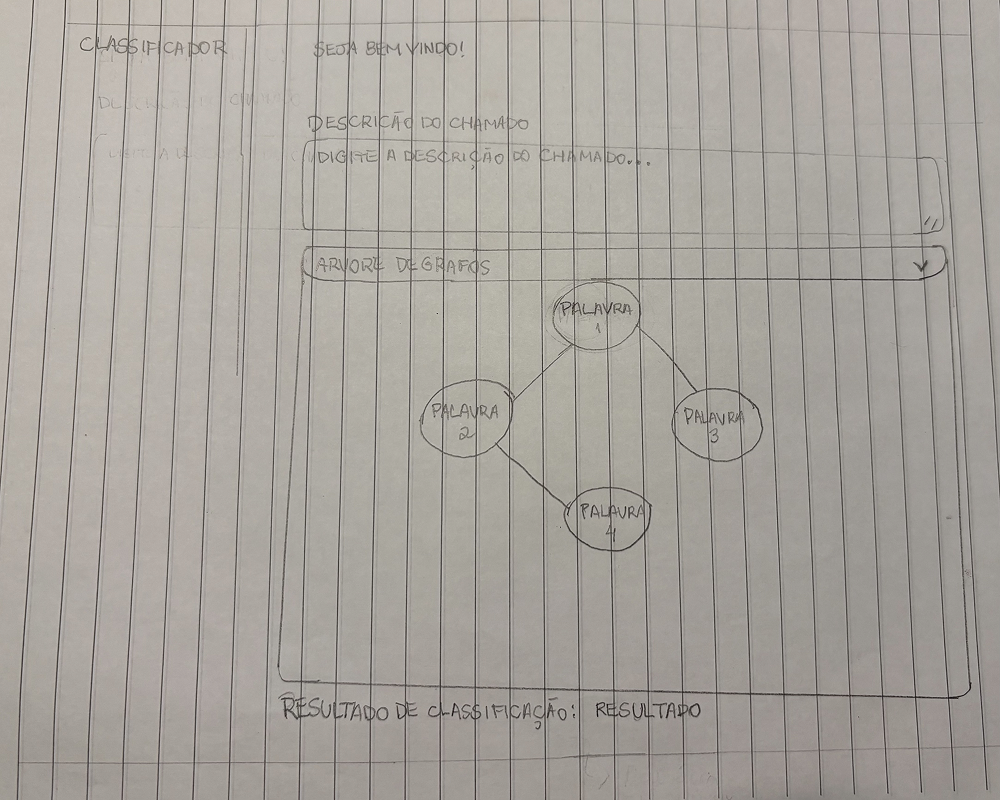
\includegraphics[width=0.75\textwidth]{imagens/baixa_agatha.png}
    \legend{Fonte: Elaborado pelos autores}
\end{figure}

\begin{figure}[H]
    \caption{Protótipo de baixa fidelidade da interface (proposta 2)}
    \label{fig:prototipo_baixa_bru}
    \centering
    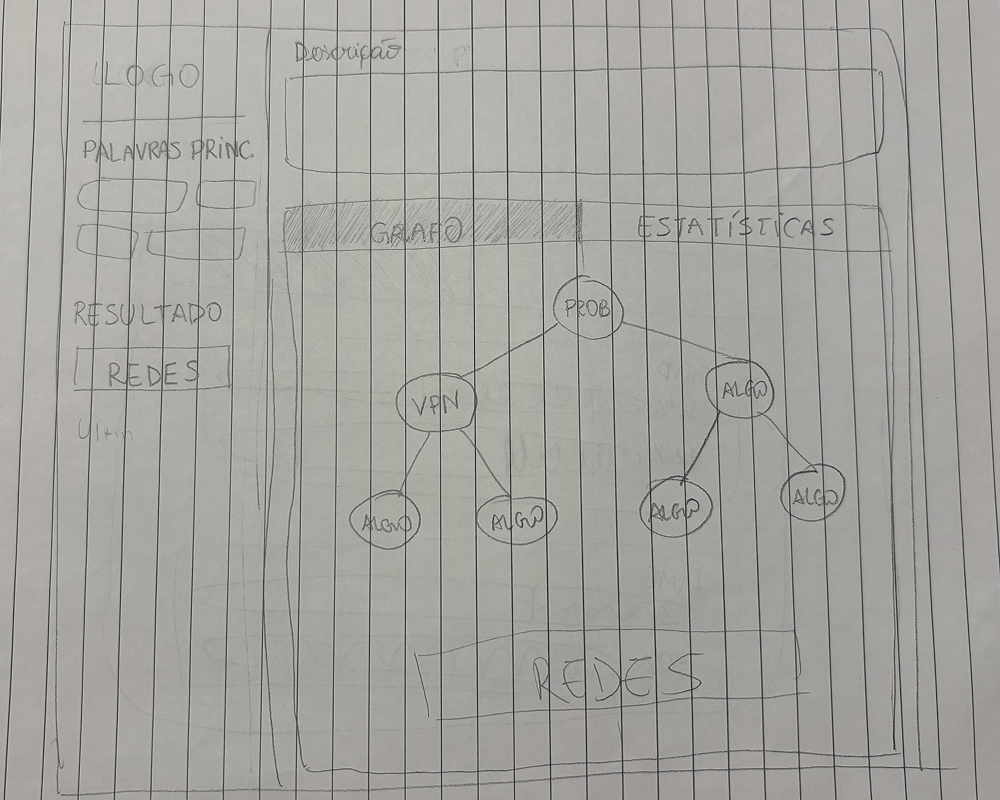
\includegraphics[width=0.75\textwidth]{imagens/baixa_bru.png}
    \legend{Fonte: Elaborado pelos autores}
\end{figure}

\begin{figure}[H]
    \caption{Protótipo de baixa fidelidade da interface (proposta 3)}
    \label{fig:prototipo_baixa_kayke}
    \centering
    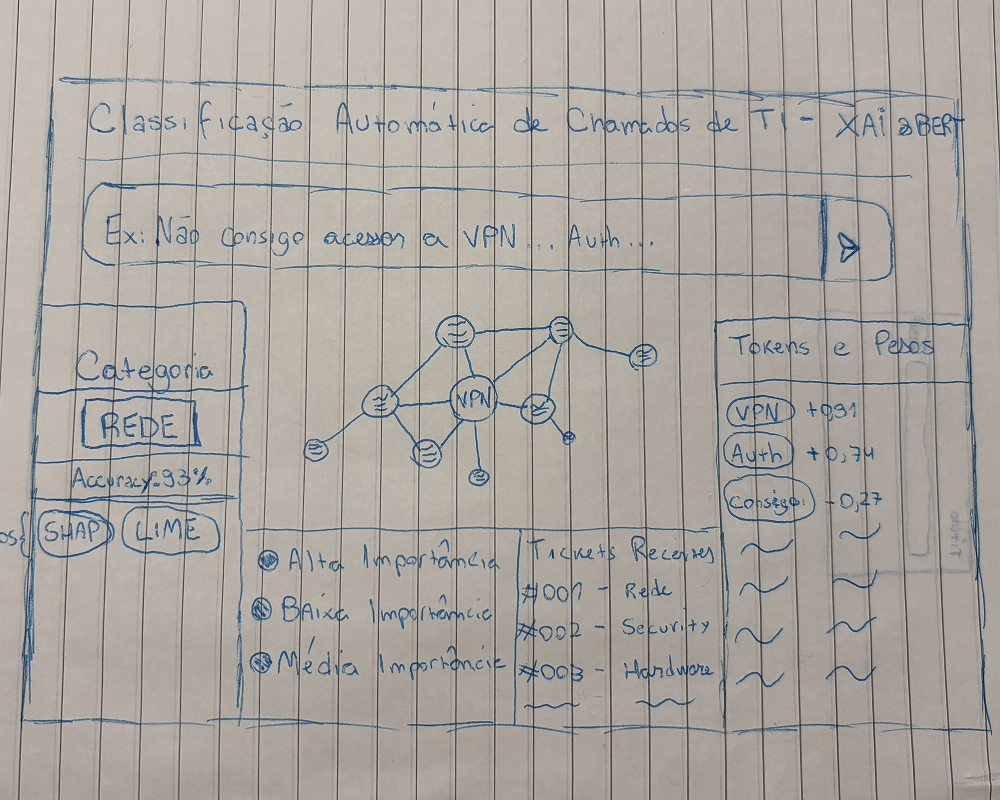
\includegraphics[width=0.75\textwidth]{imagens/baixa_kayke.png}
    \legend{Fonte: Elaborado pelos autores}
\end{figure}

\begin{figure}[H]
    \caption{Protótipo de baixa fidelidade da interface final - Tela do grafo}
    \label{fig:prototipo_baixa_grafo}
    \centering
    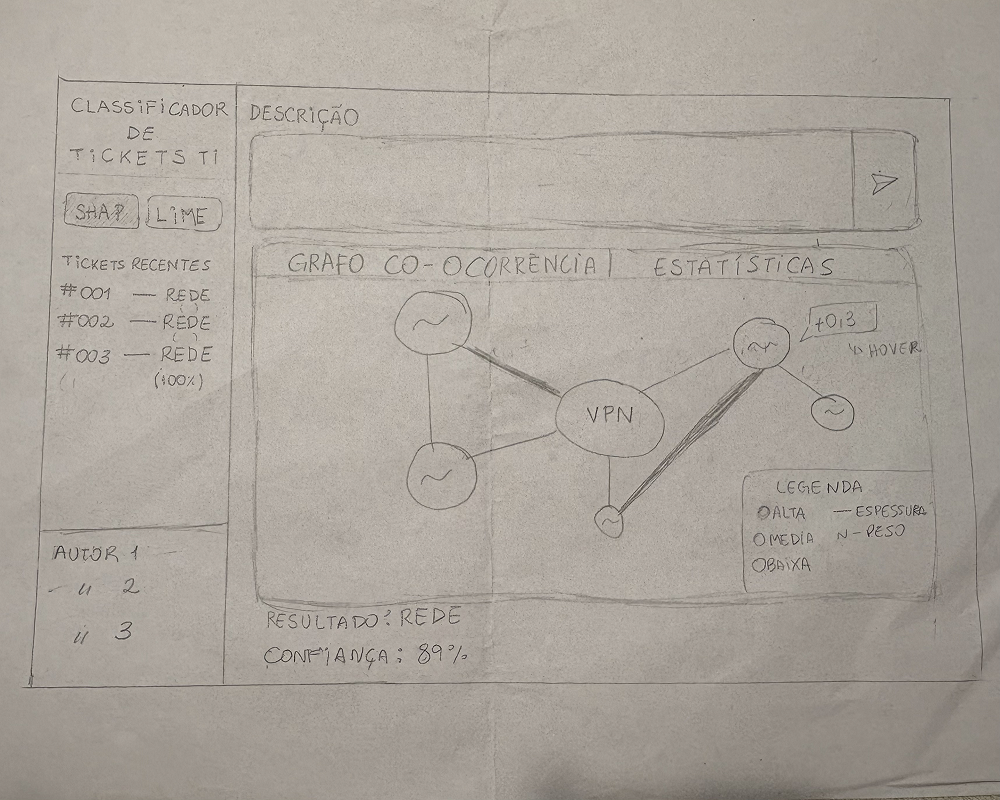
\includegraphics[width=0.75\textwidth]{imagens/baixa_grafo.png}
    \legend{Fonte: Elaborado pelos autores}
\end{figure}

\begin{figure}[H]
    \caption{Protótipo de baixa fidelidade da interface final - Tela das estatísticas}
    \label{fig:prototipo_baixa_estatisticas}
    \centering
    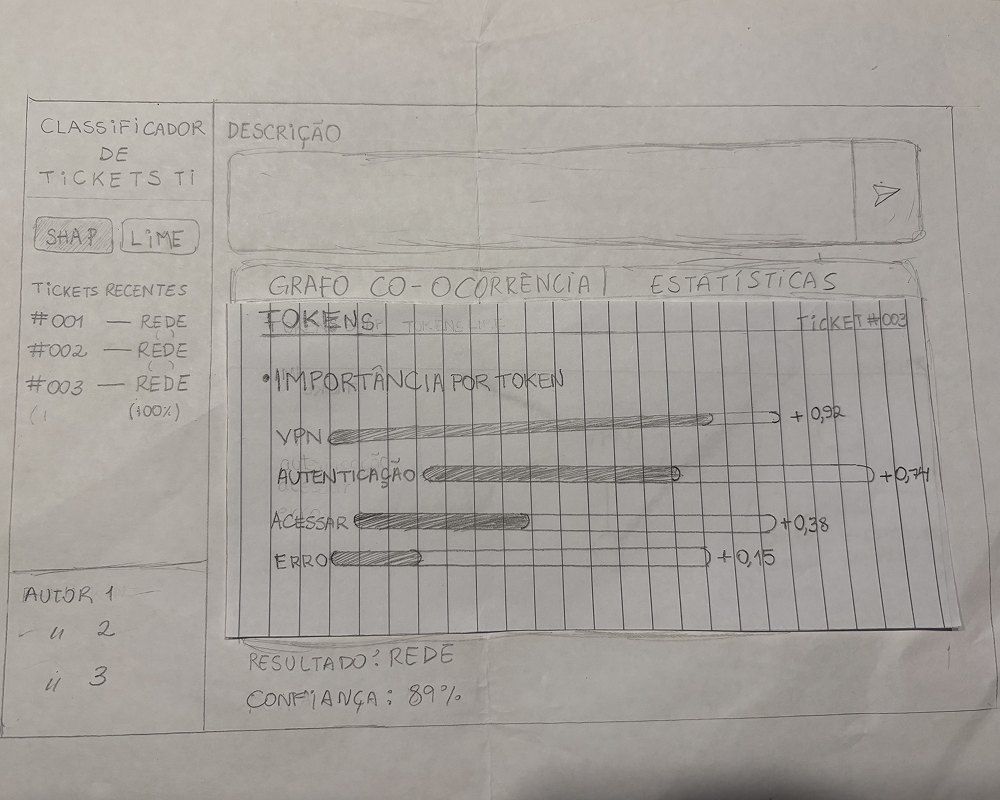
\includegraphics[width=0.75\textwidth]{imagens/baixa_estatisticas.png}
    \legend{Fonte: Elaborado pelos autores}
\end{figure}

Posteriormente, foram elaborados protótipos de média fidelidade com maior nível de detalhamento visual, com foco em validar como as explicações geradas pelo modelo seriam apresentadas de forma compreensível para os analistas de TI. 

A área central do sistema é dedicada às explicações da 
classificação, organizada em duas abas principais, ambas voltadas 
para tornar o processo decisório do modelo auditável:

\begin{itemize}
    \item \textbf{Grafo de Co-Ocorrência}: representação visual das 
    relações entre os \textit{tokens} do chamado, onde o tamanho de 
cada nó é proporcional à importância do termo (módulo do valor SHAP ou 
LIME, conforme o método escolhido em um seletor da interface), e a 
espessura das conexões indica a frequência de co-ocorrência entre os 
\textit{tokens};
    
    \item \textbf{Estatísticas}: painel que apresenta numericamente 
    a importância individual de cada \textit{token} calculada pelos 
    métodos SHAP e LIME, permitindo ao analista comparar e validar 
    as contribuições de cada termo na decisão do modelo.
\end{itemize}

A escolha por disponibilizar tanto visualizações gráficas quanto 
estatísticas numéricas busca garantir que analistas com diferentes 
perfis consigam auditar as decisões do modelo, seja por meio de 
padrões visuais no grafo ou por comparações quantitativas entre os 
valores de importância dos \textit{tokens}.

Na lateral esquerda do sistema encontra-se a seção ``Tickets 
recentes'', responsável por apresentar classificações realizadas 
anteriormente juntamente com seus respectivos níveis de confiança. 
Esse recurso permite consultar rapidamente chamados processados 
anteriormente e auxilia na análise das classificações realizadas.

Os protótipos desenvolvidos tiveram como principal objetivo verificar 
se os recursos de explicabilidade seriam apresentados de forma 
intuitiva, clara e acessível aos analistas de TI.

\begin{figure}[H]
    \caption{Protótipo de média fidelidade - visualização do grafo de co-ocorrência}
    \label{fig:prototipo_media_grafo}
    \centering
    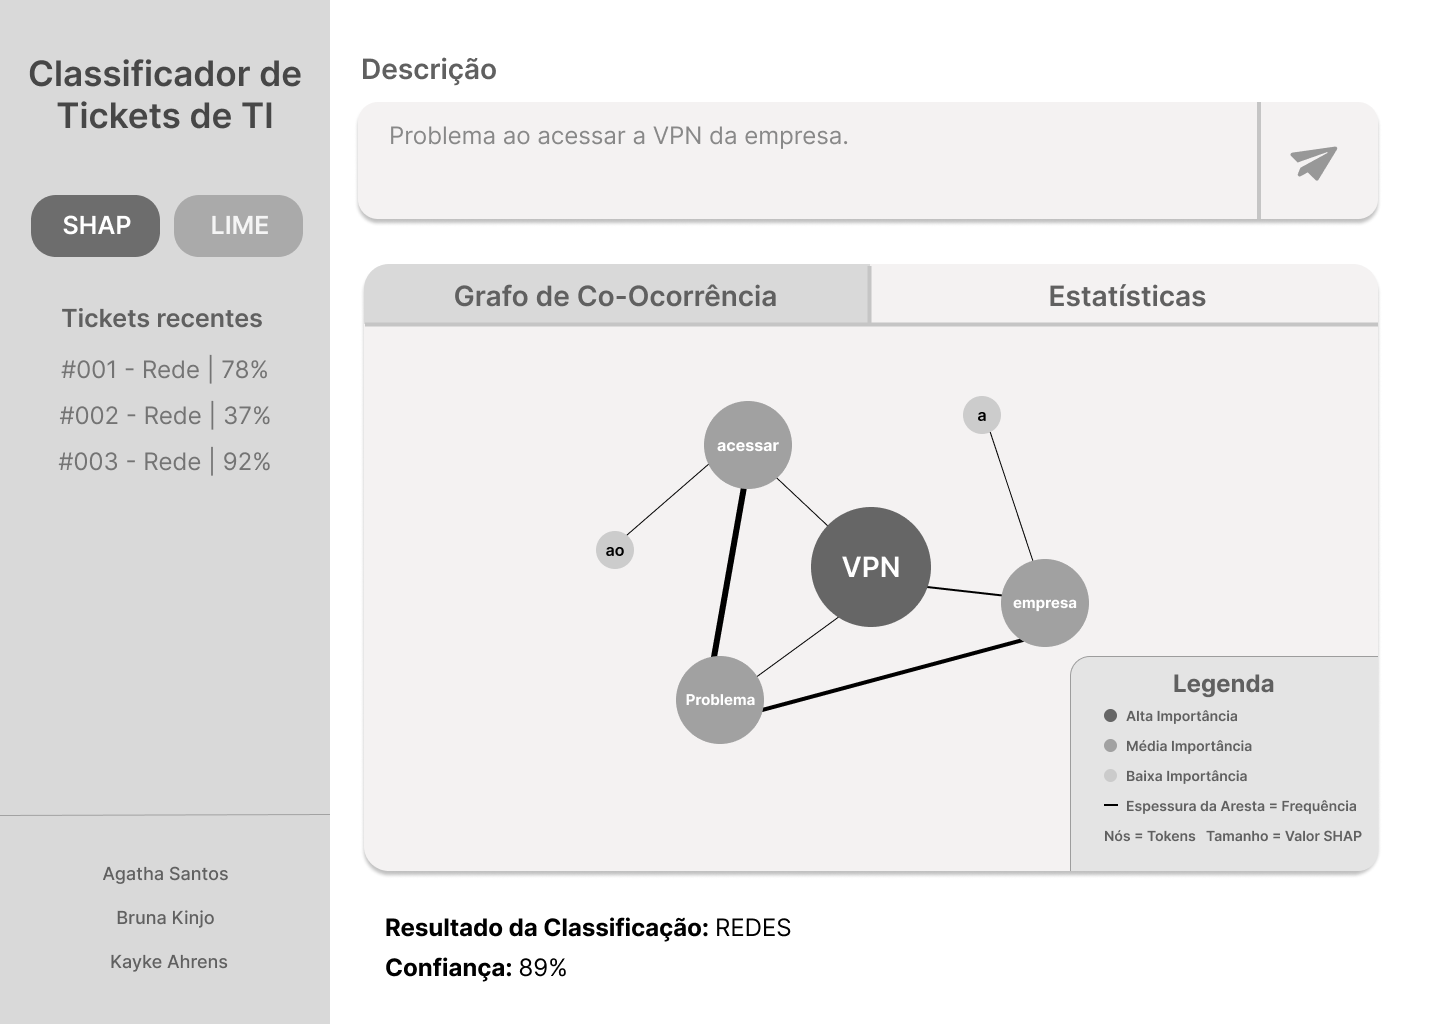
\includegraphics[width=0.75\textwidth]{imagens/grafo.png}
    \legend{Fonte: Elaborado pelos autores}
\end{figure}

\begin{figure}[H]
    \caption{Protótipo de média fidelidade - visualização estatística dos \textit{tokens}}
    \label{fig:prototipo_media_estatisticas}
    \centering
    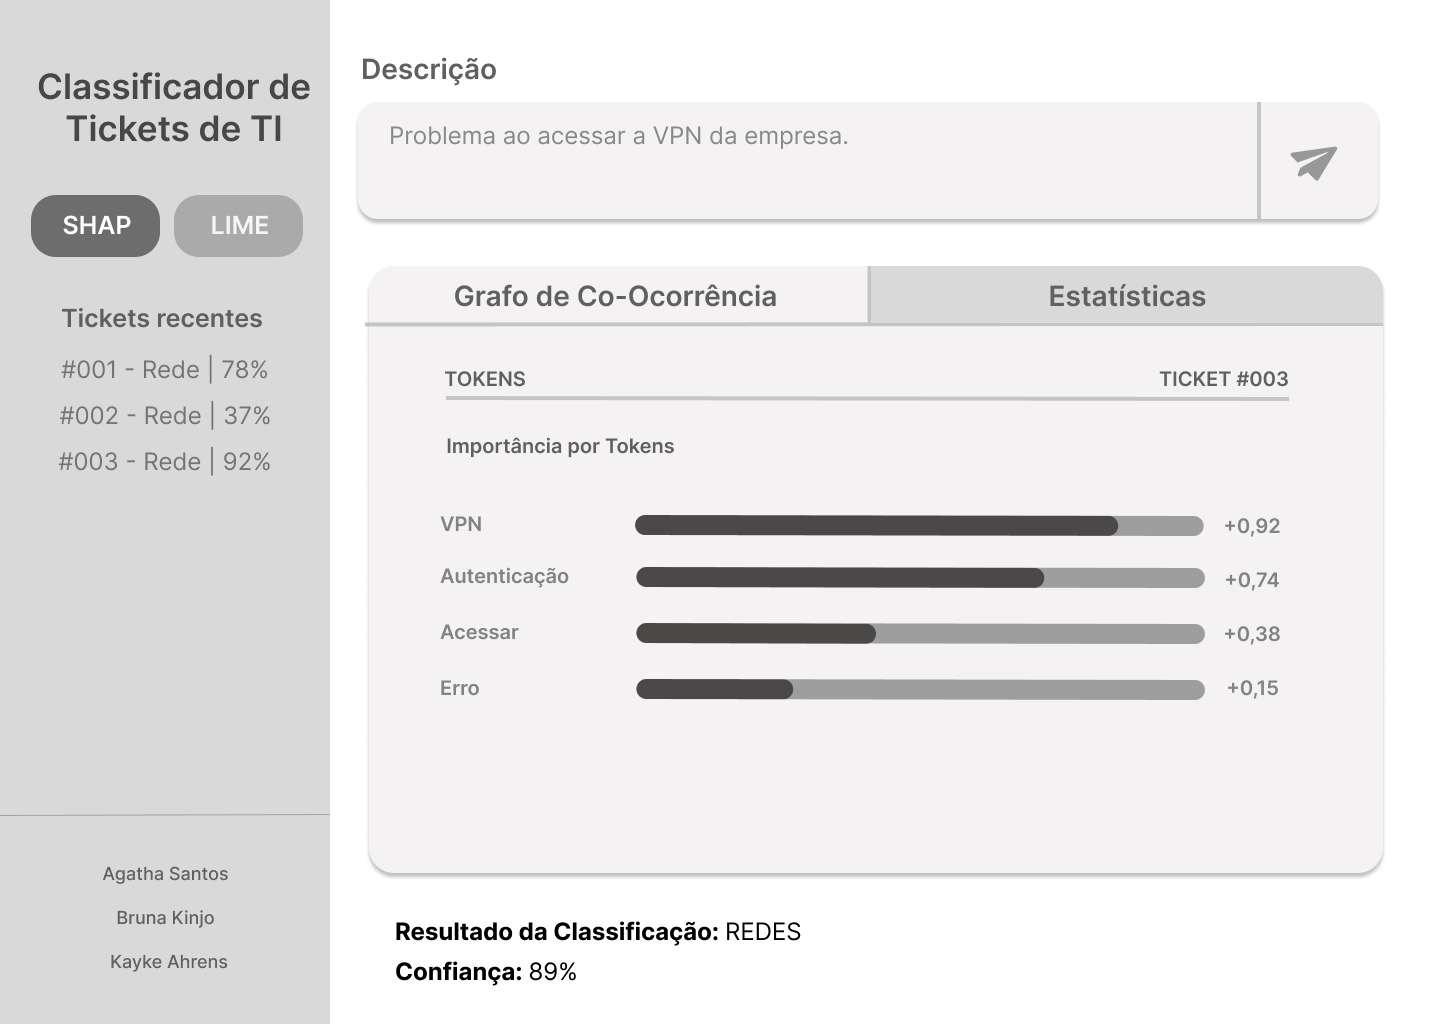
\includegraphics[width=0.75\textwidth]{imagens/estatisticas.png}
    \legend{Fonte: Elaborado pelos autores}
\end{figure}

A Figura~\ref{fig:interface_final} mostra a interface final com um chamado inventado, digitado apenas para ilustração: a interface exibe a categoria prevista e a confiança, e o grafo de co-ocorrência, com nós em azul (a favor da classe prevista) e laranja (contra), o seletor entre SHAP e LIME e a lista de chamados recentes.
\begin{figure}[H]
    \caption{Interface final: classificação de um chamado digitado e grafo de co-ocorrência}
    \label{fig:interface_final}
    \centering
    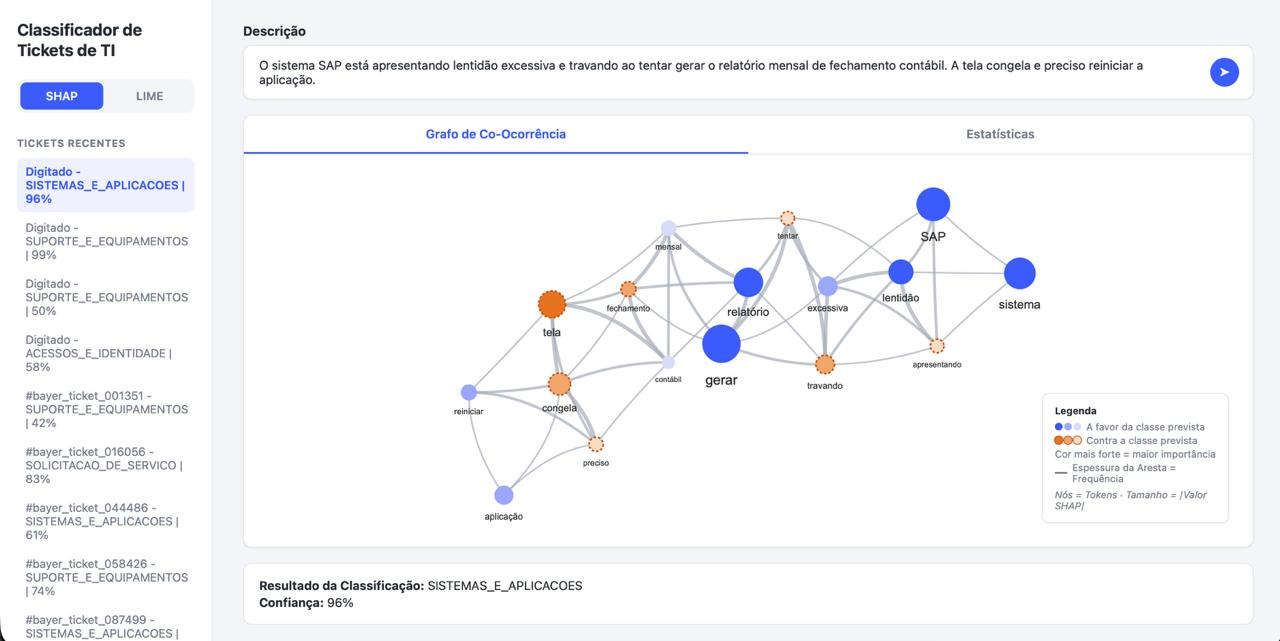
\includegraphics[width=\textwidth]{imagens/interface_final.jpg}
    \legend{Fonte: Elaborado pelos autores}
\end{figure}

\subsection{Arquitetura da solução}

A arquitetura da solução é organizada em três camadas principais:

\begin{itemize}
    \item Camada de apresentação (\textit{front-end});
    \item Camada de processamento;
    \item Camada de dados.
\end{itemize}

A camada de apresentação é responsável pela interação com o usuário final, disponibilizando os formulários de inserção de chamados, exibição das classificações, visualização dos grafos e acesso ao histórico de \textit{tickets} processados.

A camada de processamento é responsável pela execução das etapas de pré-processamento textual, inferência do modelo BERTimbau, cálculo das explicações utilizando SHAP e LIME, além da construção dos grafos de co-ocorrência.

Já a camada de dados é responsável pelo armazenamento das informações relacionadas aos chamados classificados e aos resultados gerados pelo sistema.

O fluxo geral de funcionamento da aplicação segue as seguintes etapas:

\begin{enumerate}
    \item \textbf{Entrada do modelo} — a descrição curta e a descrição completa do chamado, sem remoção de \textit{stopwords}, são passadas como um par de textos ao tokenizador do BERTimbau, que as converte em \textit{tokens} com seus respectivos IDs e máscaras de atenção. A remoção de \textit{stopwords} é usada apenas na construção do grafo.

    \item \textbf{Classificação com BERTimbau} — o modelo BERTimbau com \textit{fine-tuning} processa a sequência de \textit{tokens} e produz, a partir da representação do \textit{token} [CLS], as probabilidades de pertencimento a cada categoria. A categoria com maior probabilidade é selecionada como predição, e o índice de confiança corresponde a essa probabilidade máxima.

    \item \textbf{Cálculo de explicabilidade} — sobre o mesmo texto de entrada, são calculados os valores SHAP e as importâncias LIME. Cada \textit{token} recebe um valor numérico que representa sua contribuição para a predição: valores positivos indicam contribuição para a classe predita, e valores negativos indicam contribuição contrária.

    \item \textbf{Construção do grafo de co-ocorrência} — os \textit{tokens} do chamado são representados como nós de um grafo $G = (V, E, W, f_{\text{shap}}, f_{\text{lime}})$. As arestas conectam pares de \textit{tokens} que co-ocorrem dentro de uma janela deslizante de tamanho $w = 4$, com pesos proporcionais à frequência de co-ocorrência. Os pesos dos \textbf{nós} são determinados pelos valores SHAP e LIME calculados na etapa anterior — \textit{tokens} com maior importância, segundo o método selecionado (SHAP ou LIME), geram nós visualmente maiores na interface. O grafo é serializado em JSON, com os campos \texttt{tokens} (nós) e \texttt{arestas}, e enviado ao \textit{frontend}.

    \item \textbf{Apresentação ao analista} — a interface recebe o JSON, renderiza o grafo e exibe a categoria predita, o índice de confiança, os \textit{tokens} destacados por cor (azul, a favor da classe prevista; laranja, contra) e os valores SHAP e LIME comparativos.
\end{enumerate}

\section{Detalhes de implementação}
\subsection{Tecnologias e ferramentas}

As tecnologias e bibliotecas listadas a seguir representam as ferramentas 
utilizadas para o desenvolvimento do projeto. O detalhamento por etapa 
está na Tabela~\ref{tab:ferramentas}.

\textbf{Interface e visualização:}

\begin{itemize}
    \item \textit{React} e \textit{Vite};
    \item \textit{vis-network}, para a exibição do grafo;
    \item CSS.
\end{itemize}

\textbf{Processamento e Inteligência Artificial:}

\begin{itemize}
    \item Python;
    \item \textit{PyTorch} e \textit{Transformers}, para o BERTimbau;
    \item \textit{scikit-learn}, para o TF-IDF e o SVM;
    \item \textit{SHAP} e \textit{LIME};
    \item \textit{Flask}, para a comunicação entre a interface e o modelo.
\end{itemize}

\textbf{Ambiente de desenvolvimento:}

\begin{itemize}
    \item Git e GitHub;
    \item Máquinas locais dos integrantes do grupo.
\end{itemize}

\subsection{Funcionalidades principais}

Entre as principais funcionalidades implementadas no sistema estão:

\begin{itemize}
    \item \textbf{Funcionalidades de explicabilidade:}
    \begin{itemize}
        \item Construção de grafos de co-ocorrência;
        \item Visualização das explicações do modelo;
        \item Seleção do método de explicação (SHAP ou LIME) exibido no grafo.
    \end{itemize}
    \item \textbf{Funcionalidades de classificação e suporte:}
    \begin{itemize}
        \item Entrada do chamado em um único campo de descrição;
        \item Classificação automática de chamados de TI;
        \item Exibição da categoria prevista;
        \item Apresentação do nível de confiança da classificação;
        \item Histórico simplificado de \textit{tickets} classificados.
    \end{itemize}
\end{itemize}

\subsection{Metodologia de implementação}

A implementação do projeto seguiu uma abordagem iterativa, baseada em 
prototipação e validações incrementais.

Inicialmente foram realizados o levantamento bibliográfico, a 
definição dos requisitos e a elaboração dos protótipos da interface. 
Em seguida, foram preparados os dados, treinados os classificadores 
dos cenários A e B e implementados os módulos de explicabilidade 
(SHAP e LIME) e de construção do grafo de co-ocorrência. Por fim, 
esses módulos foram integrados à interface, que passou a gerar a 
explicação de um chamado digitado pelo \textit{pipeline} completo.


\section{Experimentos e cenários de teste}

Os experimentos seguiram os quatro cenários da Tabela~\ref{tab:cenarios}, todos sobre os mesmos conjuntos de treino, validação e teste descritos na Seção~\ref{subsubsec:dataset_finetuning}.

\subsection{Cenários A e B: classificação}

No cenário A, o \textit{baseline} SVM com TF-IDF foi treinado no conjunto de treino e avaliado no conjunto de teste, com a descrição curta e a descrição completa concatenadas como entrada. O TF-IDF usou unigramas e bigramas, frequência mínima de documento igual a 2 e escala sublinear; o classificador foi um \textit{LinearSVC} com $C = 1$, sem pesos de classe e semente 42. Assim como no BERTimbau, não foram removidas \textit{stopwords}.
No cenário B, o BERTimbau foi ajustado com a configuração da Seção~\ref{subsubsec:dataset_finetuning}. Os dois classificadores foram comparados pelas métricas da Seção~\ref{sec:metricas_avaliacao}, com destaque para o F1-macro.

\subsection{Cenário C: explicações SHAP e LIME}

As explicações foram geradas em 01/11/2026, para o modelo final, sobre uma amostra de 98 chamados do conjunto de teste: 8 acertos de cada uma das 10 classes que tiveram acertos (80 chamados) e 18 erros do modelo. A classe OUTROS não teve acertos, e por isso a amostra não tem 11 $\times$ 8 acertos. Foi necessário usar uma amostra porque SHAP e LIME explicam uma predição por vez, e explicar os 5.293 chamados do teste levaria cerca de 24 horas.

O LIME usou 500 amostras por explicação e semente 42. O SHAP (versão 0.54.1) foi calculado de forma exata nos campos de até 10 palavras (87 campos); acima disso, foi estimado por amostragem, com orçamento de 500 consultas ao modelo (79 campos). A fidelidade e a estabilidade seguiram o protocolo da Seção~\ref{subsec:criterios_validacao}; para a estabilidade, 12 chamados foram explicados 5 vezes cada. A execução completa levou cerca de 39 minutos, em CPU, em um computador Apple.

\subsection{Cenário D: grafo de co-ocorrência}

Para cada chamado explicado, construiu-se um grafo de co-ocorrência com janela deslizante de tamanho $w = 4$. As \textit{stopwords} foram removidas apenas nessa etapa, e não da entrada do modelo. O peso de cada aresta é o número de co-ocorrências do par de palavras na janela, e o peso de cada nó é o módulo da soma dos pesos que o SHAP ou o LIME atribuiu à palavra. O grafo foi avaliado por rastreabilidade, em estudos de caso (Seção~\ref{subsec:criterios_validacao}).


\section{Coleta e tratamento de dados}
\subsection{Origem e autorização de uso dos dados}
\label{subsubsec:autorizacao_dados}

Os dados utilizados neste trabalho são chamados reais de suporte
técnico cedidos por duas empresas do setor farmacêutico: Aché
Laboratórios Farmacêuticos e Bayer S.A. Os autores solicitaram o
acesso por e-mail, explicando o objetivo acadêmico do trabalho, quais
informações seriam necessárias e como os registros seriam tratados.

Não foi utilizado um conjunto de dados público. Os chamados são dados privados das duas empresas, cedidos com finalidade acadêmica e anonimizados, e por isso os textos originais não são divulgados neste trabalho.

As autorizações de uso foram concedidas pelas duas empresas por e-mail.
Os autores se comprometeram a usar os chamados apenas neste trabalho e a
anonimizá-los antes de qualquer etapa de processamento. Essas mensagens
são o registro da autorização concedida e da finalidade acadêmica do uso, e estão
reproduzidas nos Anexos~\ref{an:autorizacao_ache}
e~\ref{an:autorizacao_bayer}.

A anonimização, além de cumprir esse compromisso, alinha o trabalho ao
tratamento que a Lei Geral de Proteção de Dados Pessoais (LGPD, Lei
n.º 13.709/2018) dá aos dados anonimizados, que não são considerados
dados pessoais para os fins da lei, salvo quando a anonimização puder
ser revertida com esforços razoáveis \cite{brasil2018}. A etapa
descrita na Seção~\ref{subsubsec:dataset_finetuning} deixa de ser,
portanto, apenas uma escolha metodológica.



\subsection{\textit{Dataset} e \textit{fine-tuning}}
\label{subsubsec:dataset_finetuning}

O modelo BERTimbau, em sua versão \textit{base}, foi ajustado com chamados reais da Bayer Brasil e da Aché, obtidos mediante autorização concedida por e-mail e anonimização dos registros. O arquivo da Bayer tinha 191.350 chamados, abertos de janeiro de 2021 a agosto de 2026; após a remoção de duplicatas pelo número do chamado, o descarte de chamados sem categoria ou de categorias com menos de 100 chamados e a anonimização, restaram 189.909, dos quais 46.584 estavam em português e foram mantidos por um filtro de idioma. O arquivo da Aché tinha 9.317 chamados, todos de abril de 2026; após o descarte das categorias com menos de 100 chamados (restaram 8.758), dos chamados sem descrição (715) e de 326 cópias de uma mensagem automática de abertura por e-mail, todas da categoria de cibersegurança, restaram 7.717. As categorias das duas empresas foram harmonizadas em uma taxonomia única, e o conjunto combinado, com 54.301 chamados, passou ainda pelo descarte da classe com menos de 100 chamados (Recursos Humanos, 39 chamados) e pela remoção de 983 chamados, em 75 grupos de textos idênticos com categorias divergentes. Os resultados foram 53.279 chamados (Aché: 6.949; Bayer: 46.330), em 11 classes, entre elas a classe OUTROS.

As 11 classes da taxonomia harmonizada estão na Tabela~\ref{tab:categorias}.

\begin{table}[htb]
  \centering
  \caption{Categorias de classificação dos chamados}
  \label{tab:categorias}
  \footnotesize
  \setlength{\tabcolsep}{4pt}
  \begin{tabular}{p{5.5cm}p{6.2cm}r}
    \toprule
    Categoria & Tipo de chamado (exemplo) & Chamados no teste \\
    \midrule
    SISTEMAS\_E\_APLICACOES & Falhas e dúvidas em sistemas corporativos e aplicações & 2.458 \\
    ACESSOS\_E\_IDENTIDADE & Criação, bloqueio e revogação de acessos e contas (ex.: desligamento de colaborador) & 610 \\
    SUPORTE\_E\_EQUIPAMENTOS & Suporte a computadores e equipamentos (ex.: \textit{checklist} preventivo de salas de reunião) & 589 \\
    CONSULTA\_E\_ORIENTACAO & Dúvidas e pedidos de orientação & 555 \\
    REDES\_E\_COMUNICACOES & Rede, conectividade e comunicação & 435 \\
    SOFTWARE & Instalação e problemas de \textit{software} & 297 \\
    SOLICITACAO\_DE\_SERVICO & Pedidos de serviço (ex.: limpeza de um \textit{rack}) & 260 \\
    SERVIDORES & Chamados sobre servidores & 40 \\
    CIBERSEGURANCA & Segurança da informação & 21 \\
    AQUISICAO\_TI & Compra e licenciamento (ex.: transferência de licença do \textit{Office}) & 16 \\
    OUTROS & Demais chamados (ex.: instalação de impressoras) & 12 \\
    \bottomrule
  \end{tabular}
  \legend{Fonte: Elaborado pelos autores}
\end{table}

A base da Bayer possui, além da descrição completa, uma descrição curta, que a base da Aché não tem; nesse caso, o campo entra vazio. Ainda há chamados com texto repetido nas bases, sobretudo na Aché, o que motivou o agrupamento descrito a seguir.

O conjunto combinado foi dividido em 42.692 chamados de treino, 5.294 de validação e 5.293 de teste (proporção aproximada de 80/10/10). A divisão usou \textit{StratifiedGroupKFold} (8 partes para treino, 1 para validação e 1 para teste), estratificada pela categoria e agrupada pelo texto do chamado: chamados com texto idêntico ficam sempre na mesma parte.

O processo de \textit{fine-tuning} seguiu uma abordagem supervisionada de classificação textual. A entrada do modelo é o par formado pela descrição curta e pela descrição completa, limitado a 256 \textit{tokens}; cerca de 10,2\% dos pares ultrapassam esse limite. O treino usou 3 épocas, \textit{batch} de 16, taxa de aprendizado de $2 \times 10^{-5}$ e semente 42. Para reduzir o risco de \textit{overfitting}, fenômeno que ocorre quando o modelo aprende os dados de treino com precisão excessiva e perde a capacidade de generalizar para novos exemplos, o desempenho é acompanhado no conjunto de validação durante o treino. Não foram aplicadas técnicas de balanceamento de classes nem pesos por classe; o desbalanceamento é tratado na avaliação, com o uso do F1-macro.

% ===============================================================
% CAPÍTULO 5 - RESULTADOS E ANÁLISE
% ===============================================================
\chapter{Resultados e Análise}
\label{cap:resultados}

\section{Apresentação dos resultados}

\subsection{Desempenho da classificação (cenários A e B)}
\label{subsec:res_classificacao}

A Tabela~\ref{tab:res_teste} apresenta o desempenho dos dois classificadores no conjunto de teste, com 5.293 chamados em 4.824 grupos de texto. O BERTimbau obteve F1-macro de 0,628 e o \textit{baseline} SVM com TF-IDF, de 0,591. A acurácia dos dois é próxima (0,724 e 0,719); a diferença aparece no F1-macro, que dá o mesmo peso a todas as classes, e vem da revocação (0,611 contra 0,550), pois a precisão é parecida (0,655 contra 0,662).

\begin{table}[htb]
  \centering
  \caption{Desempenho dos classificadores no conjunto de teste}
  \label{tab:res_teste}
  \small
  \setlength{\tabcolsep}{4pt}
  \begin{tabular}{lcccc}
    \toprule
    Modelo & Acurácia & Precisão (macro) & Revocação (macro) & F1-macro \\
    \midrule
    Cenário A: SVM + TF-IDF & 0,719 & 0,662 & 0,550 & 0,591 \\
    Cenário B: BERTimbau & 0,724 & 0,655 & 0,611 & 0,628 \\
    \bottomrule
  \end{tabular}
  \legend{Fonte: Elaborado pelos autores}
\end{table}

A diferença de F1-macro a favor do BERTimbau foi de 3,7 pontos percentuais, com intervalo de confiança de 95\% de 1,0 a 6,7 (\textit{bootstrap} pareado por grupo de texto, 2.000 reamostragens). A diferença é positiva com alta confiança (probabilidade de 99,8\% nas reamostragens), mas a estimativa pontual fica abaixo do critério de 5 pontos definido no TCC1 (Seção~\ref{subsec:criterios_validacao}). Como o intervalo inclui os 5 pontos, os dados também não permitem descartar que a diferença verdadeira os alcance: a probabilidade de a diferença ser de pelo menos 5 pontos é de cerca de 21\%.

A Tabela~\ref{tab:res_classe} mostra o F1 por classe. O ganho do BERTimbau se concentra em quatro classes: SOFTWARE e SOLICITACAO\_DE\_SERVICO, com diferenças de 8,5 e 8,0 pontos e intervalos que não incluem o zero, e SERVIDORES e AQUISICAO\_TI, classes pequenas (40 e 16 chamados) com intervalos largos. Juntas, essas quatro classes respondem por 3,55 dos 3,68 pontos de diferença no F1-macro. Na maior classe, SISTEMAS\_E\_APLICACOES (46\% do teste), os dois modelos praticamente empatam (0,811 e 0,809). Nenhum dos dois acertou chamados da classe OUTROS, que tem apenas 12 chamados no teste.

\begin{table}[htb]
  \centering
  \caption{F1 por classe no conjunto de teste e diferença entre BERTimbau e SVM}
  \label{tab:res_classe}
  \footnotesize
  \setlength{\tabcolsep}{3pt}
  \begin{tabular}{lrcccc}
    \toprule
    Classe & Chamados & F1 BERTimbau & F1 SVM & Dif. (p.p.) & IC 95\% (p.p.) \\
    \midrule
SISTEMAS\_E\_APLICACOES & 2.458 & 0,811 & 0,809 & +0,3 & $-$0,8 a 1,3 \\
ACESSOS\_E\_IDENTIDADE & 610 & 0,802 & 0,775 & +2,7 & 0,5 a 8,8 \\
SUPORTE\_E\_EQUIPAMENTOS & 589 & 0,722 & 0,731 & $-$0,8 & $-$3,8 a 1,8 \\
CONSULTA\_E\_ORIENTACAO & 555 & 0,429 & 0,429 & 0,0 & $-$4,3 a 3,9 \\
REDES\_E\_COMUNICACOES & 435 & 0,726 & 0,709 & +1,7 & $-$1,3 a 5,1 \\
SOFTWARE & 297 & 0,568 & 0,483 & +8,5 & 3,2 a 13,7 \\
SOLICITACAO\_DE\_SERVICO & 260 & 0,440 & 0,360 & +8,0 & 1,8 a 14,1 \\
SERVIDORES & 40 & 0,667 & 0,613 & +5,4 & $-$4,9 a 17,3 \\
CIBERSEGURANCA & 21 & 0,900 & 0,923 & $-$2,3 & $-$8,8 a 0,0 \\
AQUISICAO\_TI & 16 & 0,839 & 0,667 & +17,2 & $-$7,0 a 44,8 \\
OUTROS & 12 & 0,000 & 0,000 & 0,0 & 0,0 a 0,0 \\
    \bottomrule
  \end{tabular}
  \legend{Fonte: Elaborado pelos autores. IC: intervalo de confiança por \textit{bootstrap} pareado; p.p.: pontos percentuais.}
\end{table}

A Tabela~\ref{tab:res_empresa} separa o teste por empresa. O F1-macro de cada empresa é calculado sobre as classes presentes em seus chamados (7 na Aché e 9 na Bayer). Os dois modelos têm desempenho muito maior na Aché, e a diferença a favor do BERTimbau é de 1,3 ponto na Aché, com intervalo que inclui o zero, e de 4,0 pontos na Bayer. Como a Bayer reúne 86\% dos chamados de teste, o resultado geral reflete sobretudo essa empresa. Os 716 chamados da Aché formam apenas 337 grupos de texto, e um desses textos, um roteiro de desligamento de colaborador, aparece em 298 chamados da classe ACESSOS\_E\_IDENTIDADE, todos classificados corretamente pelos dois modelos. 
Sem esse grupo, restam 418 chamados da Aché, ainda nas mesmas 7 classes, e o F1-macro da empresa fica em 0,901 (BERTimbau) e 0,889 (SVM). A diferença continua de 1,3 ponto, o que mostra que esse grupo repetido não explica o resultado da Aché nem a diferença entre os modelos.

\begin{table}[htb]
  \centering
  \caption{Desempenho no conjunto de teste, por empresa de origem}
  \label{tab:res_empresa}
  \footnotesize
  \setlength{\tabcolsep}{4pt}
  \begin{tabular}{lrrcccc}
    \toprule
    Subconjunto & Chamados & Grupos & F1 BERTimbau & F1 SVM & Dif. (p.p.) & IC de 95\% (p.p.) \\
    \midrule
    Aché & 716 & 337 & 0,911 & 0,897 & +1,3 & $-$3,1 a 5,9 \\
    Bayer & 4.577 & 4.487 & 0,515 & 0,474 & +4,0 & 1,6 a 6,5 \\
    Total & 5.293 & 4.824 & 0,628 & 0,591 & +3,7 & 1,0 a 6,7 \\
    \bottomrule
  \end{tabular}
  \legend{Fonte: Elaborado pelos autores. Grupos: conjuntos de chamados com texto idêntico.}
\end{table}

No conjunto de validação, a diferença segue a mesma direção. Após retirar um bloco de 491 chamados de SUPORTE\_E\_EQUIPAMENTOS com o mesmo texto (um \textit{checklist} preventivo de salas de reunião, que o SVM classificou como REDES\_E\_COMUNICACOES e o BERTimbau como SUPORTE\_E\_EQUIPAMENTOS), restam 4.803 chamados, nos quais o F1-macro foi de 0,591 para o BERTimbau e 0,555 para o SVM, uma diferença de 3,5 pontos (intervalo de 95\% de 1,3 a 6,1). Na validação inteira, de 5.294 chamados, a diferença seria de 11,9 pontos, inflada por esse único texto.

A Figura~\ref{fig:matriz_confusao} mostra a matriz de confusão do BERTimbau no teste. Os erros mais frequentes ocorrem entre CONSULTA\_E\_ORIENTACAO e SISTEMAS\_E\_APLICACOES (180 chamados previstos como a segunda e 146 no sentido inverso), seguidos de SOLICITACAO\_DE\_SERVICO previstos como SISTEMAS\_E\_APLICACOES (78) e de SISTEMAS\_E\_APLICACOES previstos como SUPORTE\_E\_EQUIPAMENTOS (76). As classes de menor F1 são CONSULTA\_E\_ORIENTACAO (0,429), SOLICITACAO\_DE\_SERVICO (0,440) e OUTROS (0,000). Uma possível explicação, que este trabalho não testou, é que essas classes descrevem o tipo de pedido, e não o sistema ou equipamento envolvido, e por isso se sobrepõem às demais.

\begin{figure}[H]
    \caption{Matriz de confusão do BERTimbau no conjunto de teste, normalizada por classe real}
    \label{fig:matriz_confusao}
    \centering
    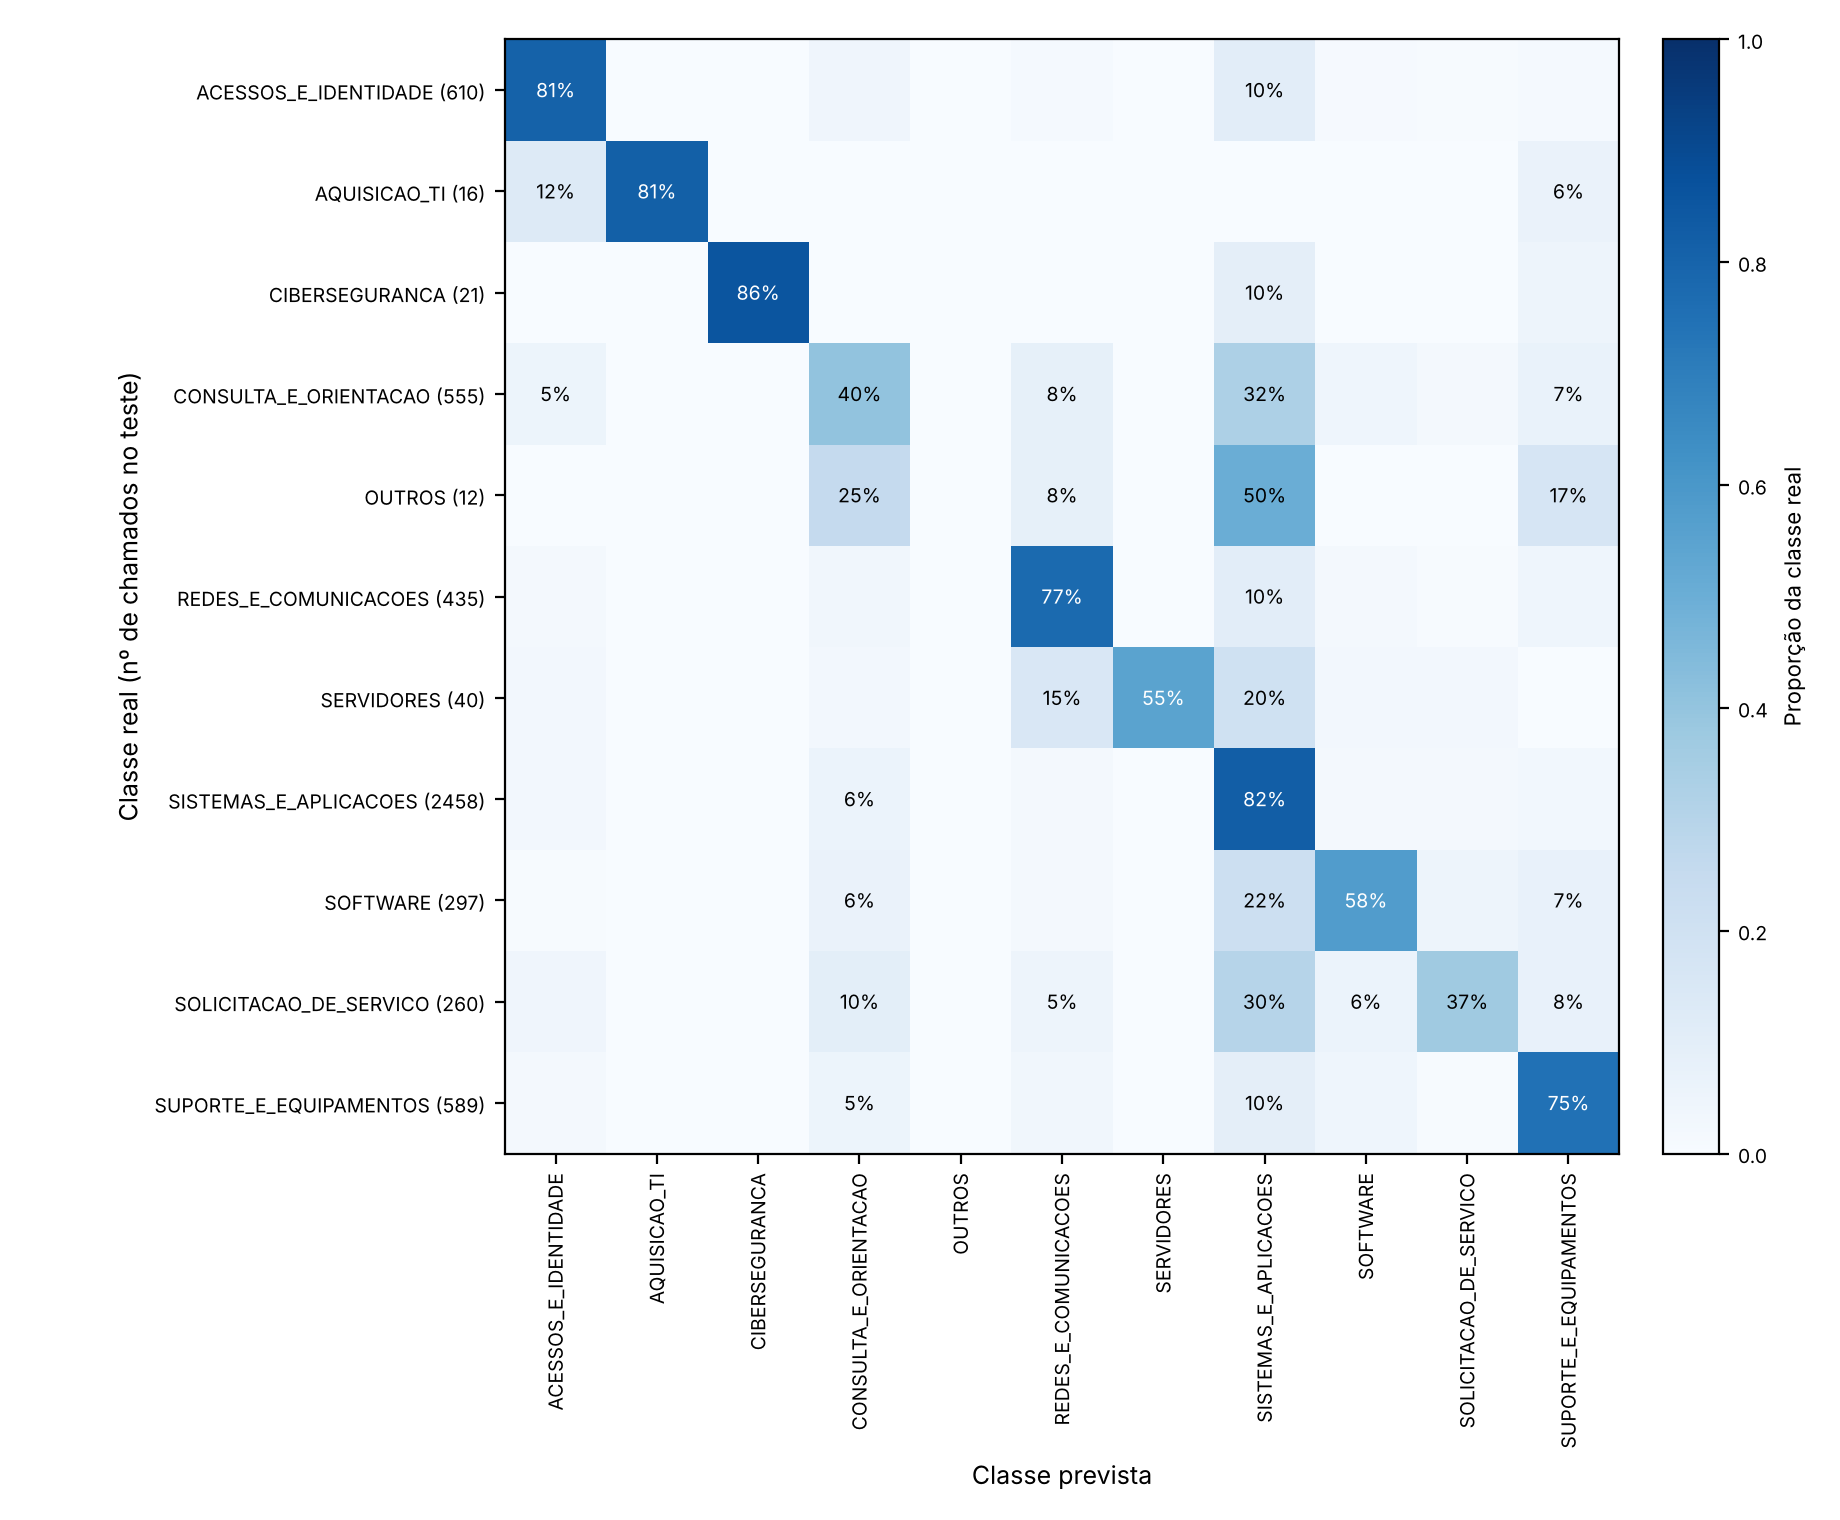
\includegraphics[width=0.9\textwidth]{imagens/matriz_confusao_teste.png}
    \legend{Fonte: Elaborado pelos autores}
\end{figure}

\subsection{Explicabilidade: SHAP e LIME (cenário C)}
As explicações do SHAP e do LIME foram geradas para os 98 chamados da amostra (Seção~\ref{subsec:criterios_validacao}). Em CPU, o LIME levou 964 segundos (cerca de 16 minutos) e o SHAP, 616 segundos (cerca de 10 minutos). No SHAP, a soma dos pesos das palavras com a probabilidade-base reproduziu a probabilidade do chamado em todas as explicações, com erro máximo da ordem de $10^{-15}$. No LIME, o $R^2$ do modelo linear local teve mediana de 0,68, com mínimo de 0,11.

\subsubsection{Fidelidade}
\label{subsubsec:res_fidelidade}

A Tabela~\ref{tab:res_fidelidade} traz a fidelidade dos dois métodos nos 98 chamados. Na \textit{comprehensiveness}, mede-se a queda da probabilidade da classe prevista ao retirar as palavras apontadas pelo método (quanto maior, melhor); na \textit{sufficiency}, a queda ao manter apenas essas palavras (quanto menor, melhor); o Tau-LOO é a correlação de Kendall entre o peso de cada palavra e a queda de probabilidade ao retirá-la sozinha (quanto maior, melhor). As duas primeiras são comparadas à queda obtida com palavras sorteadas.

\begin{table}[htb]
  \centering
  \caption{Fidelidade das explicações do SHAP e do LIME nos 98 chamados da amostra}
  \label{tab:res_fidelidade}
  \small
  \begin{tabular}{p{4.6cm}lccc}
    \toprule
    Medida & Método & Explicação & Aleatório & Acima do acaso \\
    \midrule
    \textit{Comprehensiveness} (maior é melhor) & LIME & 0,542 & 0,192 & 94 de 98 \\
     & SHAP & 0,526 & 0,182 & 96 de 98 \\
    \addlinespace
    \textit{Sufficiency} (menor é melhor) & LIME & 0,019 & 0,309 & 96 de 98 \\
     & SHAP & 0,010 & 0,317 & 93 de 98 \\
    \addlinespace
    Tau-LOO (maior é melhor) & LIME & 0,412 & -- & 95 de 98 \\
     & SHAP & 0,353 & -- & 95 de 98 \\
    \bottomrule
  \end{tabular}
  \legend{Fonte: Elaborado pelos autores. Valores médios por chamado. Cinco sorteios aleatórios por chamado, semente 42. ``Acima do acaso'': chamados em que a explicação supera o sorteio. No Tau-LOO não há linha de base aleatória, e a última coluna indica os chamados com valor positivo.}
\end{table}

Os dois métodos ficam bem acima do acaso nas três medidas. Retirar as palavras apontadas reduz a probabilidade da classe prevista em 0,54 (LIME) e 0,53 (SHAP), contra 0,19 e 0,18 ao retirar palavras sorteadas, e manter só as palavras apontadas deixa a probabilidade quase inalterada (queda de 0,02 e 0,01), contra 0,31 e 0,32 com palavras sorteadas. As diferenças entre os métodos são pequenas: o LIME tem valores um pouco maiores na \textit{comprehensiveness} e no Tau-LOO (0,54 contra 0,53 e 0,41 contra 0,35), e o SHAP, uma queda menor na \textit{sufficiency} (0,010 contra 0,019). Para comparar os métodos nos mesmos chamados, calculou-se a diferença SHAP menos LIME em cada chamado, com intervalo de confiança de 95\% por \textit{bootstrap} sobre os chamados (5.000 reamostragens, semente 42). Na \textit{comprehensiveness}, a diferença média foi de $-0{,}015$ (intervalo de $-0{,}037$ a 0,006), e na \textit{sufficiency}, de $-0{,}008$ (intervalo de $-0{,}033$ a 0,012); os dois intervalos incluem o zero, e os dados não distinguem os métodos nessas medidas. No Tau-LOO, a diferença foi de $-0{,}059$ (intervalo de $-0{,}090$ a $-0{,}027$), ou seja, o LIME teve correlação maior com o efeito de retirar cada palavra.

\subsubsection{Estabilidade}
\label{subsubsec:res_estabilidade}

A estabilidade foi medida em 12 chamados com ao menos oito palavras distintas, explicados 5 vezes cada, com sementes diferentes (Tabela~\ref{tab:res_estabilidade}). Em 3 desses chamados, todos os campos têm até 10 palavras e o SHAP foi calculado de forma exata, sem sorteio, de modo que a explicação é idêntica nas cinco repetições (estabilidade 1 por construção). Nos outros 9, ao menos um campo foi estimado por amostragem, com orçamento de 500 consultas, e o SHAP variou de uma repetição para outra.

\begin{table}[htb]
  \centering
  \caption{Estabilidade das explicações do SHAP e do LIME em 12 chamados, com 5 repetições}
  \label{tab:res_estabilidade}
  \small
  \begin{tabular}{p{3.9cm}rccc}
    \toprule
    Método & Chamados & Jaccard (acaso) & Spearman & Topo igual (acaso) \\
    \midrule
    LIME & 12 & 0,659 (0,213) & 0,774 & 0,950 (0,062) \\
    SHAP, todos & 12 & 0,638 (0,213) & 0,736 & 0,758 (0,062) \\
    SHAP, só amostragem & 9 & 0,517 (0,135) & 0,648 & 0,678 (0,043) \\
    \bottomrule
  \end{tabular}
  \legend{Fonte: Elaborado pelos autores. Valores médios por chamado. Jaccard: das 5 palavras mais relevantes entre as repetições. ``Topo igual'': fração das repetições com a mesma palavra no topo. Entre parênteses, o valor esperado ao acaso. ``Só amostragem'' exclui os 3 chamados em que o SHAP foi exato.}
\end{table}

Os dois métodos ficam acima do acaso nas três medidas, mas nenhum é perfeitamente estável. O LIME manteve a mesma palavra no topo em 95\% das repetições e teve Jaccard de 0,659. O SHAP teve Jaccard de 0,638 e a mesma palavra no topo em 76\% das repetições; considerando só os 9 chamados em que houve amostragem, os valores caem para 0,517 e 68\%. Nos 9 chamados em que houve amostragem, a comparação é direta, com os mesmos chamados nos dois métodos: o LIME teve Jaccard de 0,546 contra 0,517 do SHAP, Spearman de 0,706 contra 0,648 e a mesma palavra no topo em 93\% das repetições contra 68\%. Nessa amostra, portanto, o SHAP estimado por amostragem, com 500 consultas, não foi mais estável que o LIME, e só o cálculo exato dá estabilidade total ao SHAP. Como são apenas 12 chamados e não houve teste estatístico, o resultado é indicativo.

\subsubsection{Concordância entre SHAP e LIME}
\label{subsubsec:res_concordancia}

A concordância compara, para cada um dos 98 chamados, as palavras que o SHAP e o LIME apontaram como importantes para a classe prevista. Como os pesos estão em escalas diferentes (probabilidade no SHAP, coeficiente do modelo linear local no LIME), a comparação usa a ordem e o sinal das palavras, e não o valor dos pesos. A Tabela~\ref{tab:res_concordancia} mostra o resultado, ao lado do valor esperado ao acaso.

\begin{table}[htb]
  \centering
  \caption{Concordância entre SHAP e LIME nos 98 chamados da amostra}
  \label{tab:res_concordancia}
  \small
  \begin{tabular}{p{5.6cm}ccc}
    \toprule
    Medida & Resultado & Ao acaso & Chamados acima do acaso \\
    \midrule
    Correlação de Spearman entre os pesos (média) & 0,704 & 0,000 & 98 de 98 \\
    Jaccard das 5 palavras mais relevantes (média) & 0,575 & 0,226 & 91 de 96 \\
    Mesma palavra no topo (fração de chamados) & 0,714 (70 de 98) & 0,068 & -- \\
    Palavras com o mesmo sinal (média) & 0,792 & 0,500 & 97 de 98 \\
    \bottomrule
  \end{tabular}
  \legend{Fonte: Elaborado pelos autores. O Jaccard considera apenas os 96 chamados com mais de 5 palavras.}
\end{table}

Nas quatro medidas, os dois métodos concordam bem acima do acaso, mas longe da concordância total. Em 70 dos 98 chamados (71\%) os dois colocam a mesma palavra no topo, contra 7\% esperados ao acaso, e a mediana da correlação de Spearman é 0,757. A concordância não indica qual dos métodos está certo, apenas que apontam as mesmas palavras; a fidelidade de cada um é tratada à parte.

A Tabela~\ref{tab:res_concordancia_grupos} separa os chamados por forma de cálculo do SHAP e por acerto do modelo. A concordância é maior nos 27 chamados em que o SHAP foi calculado de forma exata (Spearman de 0,864) do que nos 71 em que houve amostragem (0,643). Os chamados do primeiro grupo são os mais curtos, então os dados não separam o efeito do método de cálculo do efeito do tamanho do texto. Em todos os chamados, a correlação entre o número de palavras e a concordância de Spearman é de $-0{,}67$ ($p < 0{,}001$): quanto mais palavras, menos os dois métodos concordam. Já entre acertos e erros do modelo, a concordância é praticamente a mesma (Spearman de 0,704 nos dois grupos), com amostra de erros pequena (18 chamados).

\begin{table}[htb]
  \centering
  \caption{Concordância entre SHAP e LIME por subconjunto de chamados}
  \label{tab:res_concordancia_grupos}
  \small
  \begin{tabular}{lrcccc}
    \toprule
    Subconjunto & Chamados & Spearman & Jaccard & Mesmo topo & Mesmo sinal \\
    \midrule
    Todos & 98 & 0,704 & 0,575 & 0,714 & 0,792 \\
    SHAP exato & 27 & 0,864 & 0,762 & 0,741 & 0,899 \\
    SHAP por amostragem & 71 & 0,643 & 0,509 & 0,704 & 0,752 \\
    Acertos do modelo & 80 & 0,704 & 0,583 & 0,700 & 0,788 \\
    Erros do modelo & 18 & 0,704 & 0,535 & 0,778 & 0,815 \\
    \bottomrule
  \end{tabular}
  \legend{Fonte: Elaborado pelos autores. Valores médios por chamado; ``Mesmo topo'' é a fração de chamados com a mesma palavra no topo. O Jaccard considera apenas chamados com mais de 5 palavras (25 no SHAP exato, 71 na amostragem, 79 nos acertos e 17 nos erros).}
\end{table}

\subsection{Grafo de co-ocorrência (cenário D)}
O grafo foi avaliado por rastreabilidade em três chamados da amostra de 98, escolhidos para cobrir situações diferentes: um acerto com vocabulário típico da classe (caso 1), um erro do modelo (caso 2) e um acerto em que os dois métodos divergem nas palavras secundárias (caso 3). A Tabela~\ref{tab:res_casos} resume os três, e as Figuras~\ref{fig:grafo_caso1}, \ref{fig:grafo_caso2} e~\ref{fig:grafo_caso3} mostram os grafos na interface.

\begin{table}[htb]
  \centering
  \caption{Chamados usados nos estudos de caso do grafo}
  \label{tab:res_casos}
  \footnotesize
  \begin{tabular}{cp{3.8cm}p{4.9cm}cc}
    \toprule
    Caso & Chamado & Classe real $\rightarrow$ prevista & Conf. & Nós/arestas \\
    \midrule
    1 & ache\_ticket\_001118 & AQUISICAO\_TI $\rightarrow$ igual & 0,91 & 16/42 \\
    2 & bayer\_ticket\_001351 & OUTROS $\rightarrow$ SUPORTE\_E\_EQUIPAMENTOS & 0,42 & 4/6 \\
    3 & bayer\_ticket\_016056 & SOLICITACAO\_DE\_SERVICO $\rightarrow$ igual & 0,83 & 10/25 \\
    \bottomrule
  \end{tabular}
  \legend{Fonte: Elaborado pelos autores.}
\end{table}

Nos três casos, a rastreabilidade se cumpriu. Cada nó corresponde a uma palavra que aparece no texto do chamado, com o campo em que ocorre e os pesos do SHAP e do LIME; cada aresta liga dois nós existentes e tem como peso o número de vezes que o par co-ocorre na janela deslizante de 4 palavras, valor que pode ser recalculado a partir do texto.

No caso 1, o chamado pede a transferência de uma licença do pacote \textit{Office} para outra pessoa. As duas palavras de maior peso a favor da classe são as mesmas nos dois métodos, \textit{licença} (SHAP de 0,476; LIME de 0,447) e \textit{office} (0,151 e 0,138), e são o vocabulário esperado para a aquisição de \textit{software}. O grafo mostra \textit{licença} como o maior nó, ligado a \textit{office} e \textit{pacote}.

\begin{figure}[H]
    \caption{Grafo de co-ocorrência do caso 1 (ache\_ticket\_001118), com pesos SHAP}
    \label{fig:grafo_caso1}
    \centering
    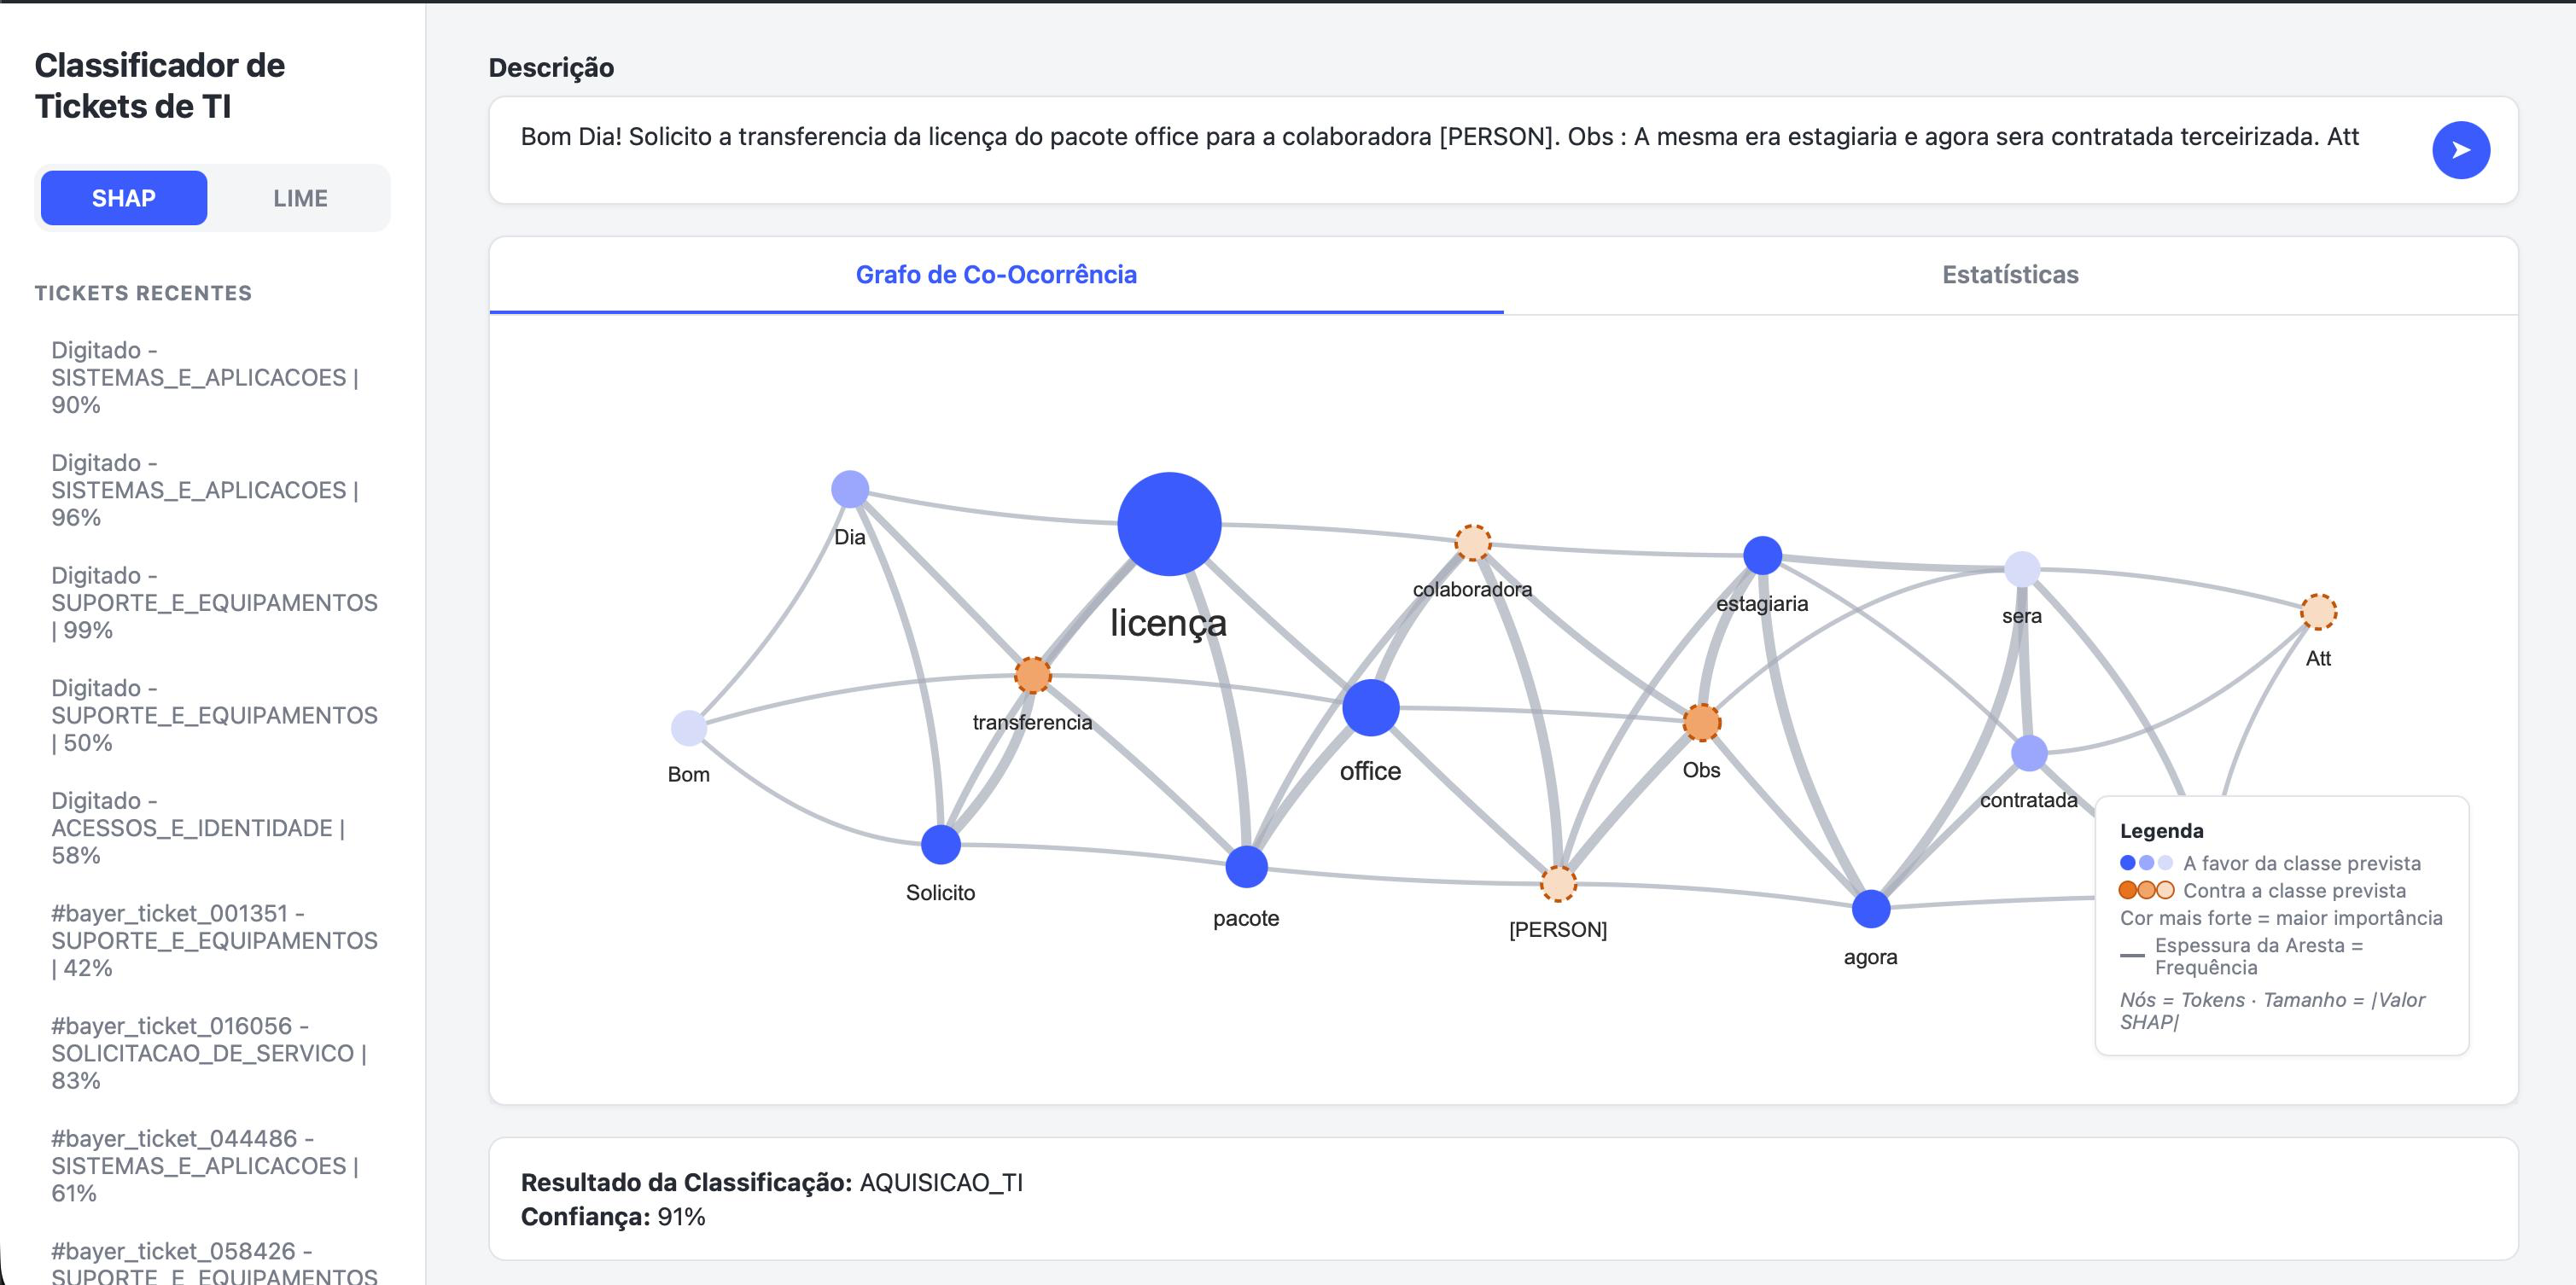
\includegraphics[width=\textwidth]{imagens/grafo_caso1_ache_001118.png}
    \legend{Fonte: Elaborado pelos autores}
\end{figure}

No caso 2, o chamado tem uma única frase, sobre a instalação de duas impressoras, e a categoria real é OUTROS; o modelo previu SUPORTE\_E\_EQUIPAMENTOS com confiança de 0,42. O grafo tem apenas 4 nós. A palavra de maior peso, \textit{Rena}, a marca de uma das impressoras, pesa contra a classe prevista (SHAP de $-$0,248; LIME de $-$0,290), assim como \textit{impressoras} ($-$0,101 e $-$0,077), enquanto o marcador de anonimização \textit{[PERSON]} pesa a favor (0,124 e 0,144). A explicação mostra que a decisão se apoiou em muito pouca evidência e que um marcador de anonimização influenciou a previsão, o que um analista pode questionar.

\begin{figure}[H]
    \caption{Grafo de co-ocorrência do caso 2 (bayer\_ticket\_001351), com pesos SHAP}
    \label{fig:grafo_caso2}
    \centering
    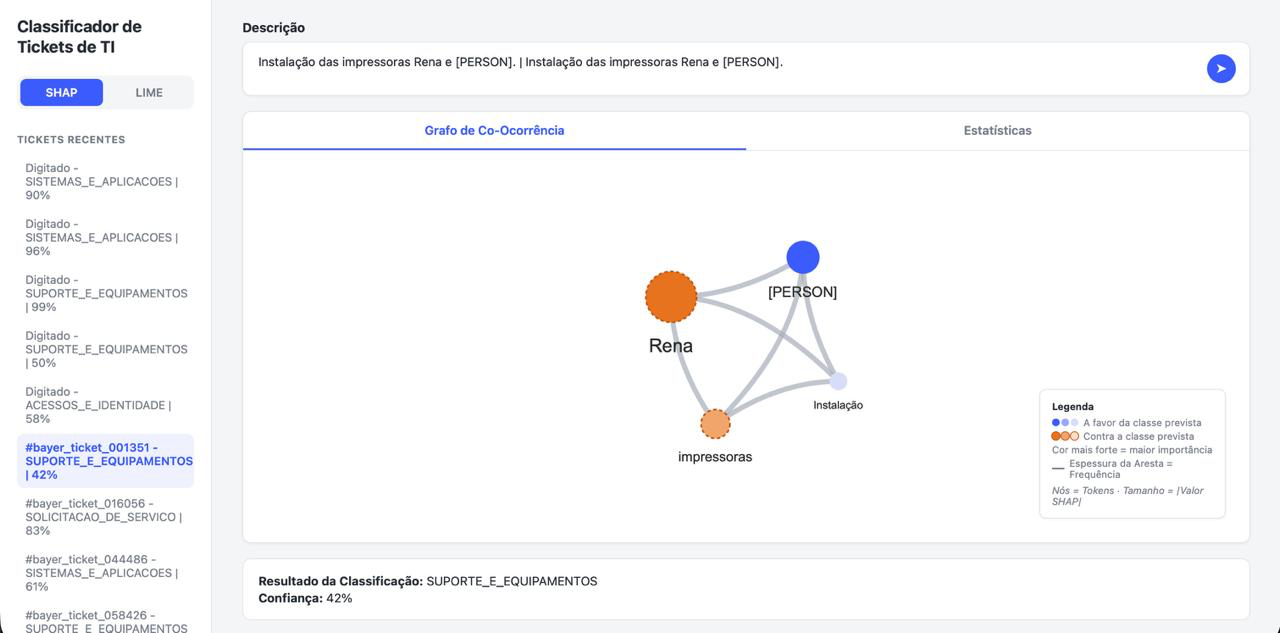
\includegraphics[width=\textwidth]{imagens/grafo_caso2_bayer_001351.png}
    \legend{Fonte: Elaborado pelos autores}
\end{figure}

No caso 3, o chamado pede a limpeza de um \textit{rack}. Os dois métodos concordam na palavra de maior peso, \textit{Favor} (SHAP de 0,322; LIME de 0,346), típica de um pedido de serviço. Nas demais palavras, porém, divergem: \textit{limpeza} tem peso de 0,165 no SHAP e de apenas 0,002 no LIME. O grafo, construído com os pesos do SHAP, e o do LIME, portanto, destacam conjuntos diferentes de palavras além da primeira, o que o analista pode verificar alternando o método na interface.

\begin{figure}[H]
    \caption{Grafo de co-ocorrência do caso 3 (bayer\_ticket\_016056), com pesos SHAP}
    \label{fig:grafo_caso3}
    \centering
    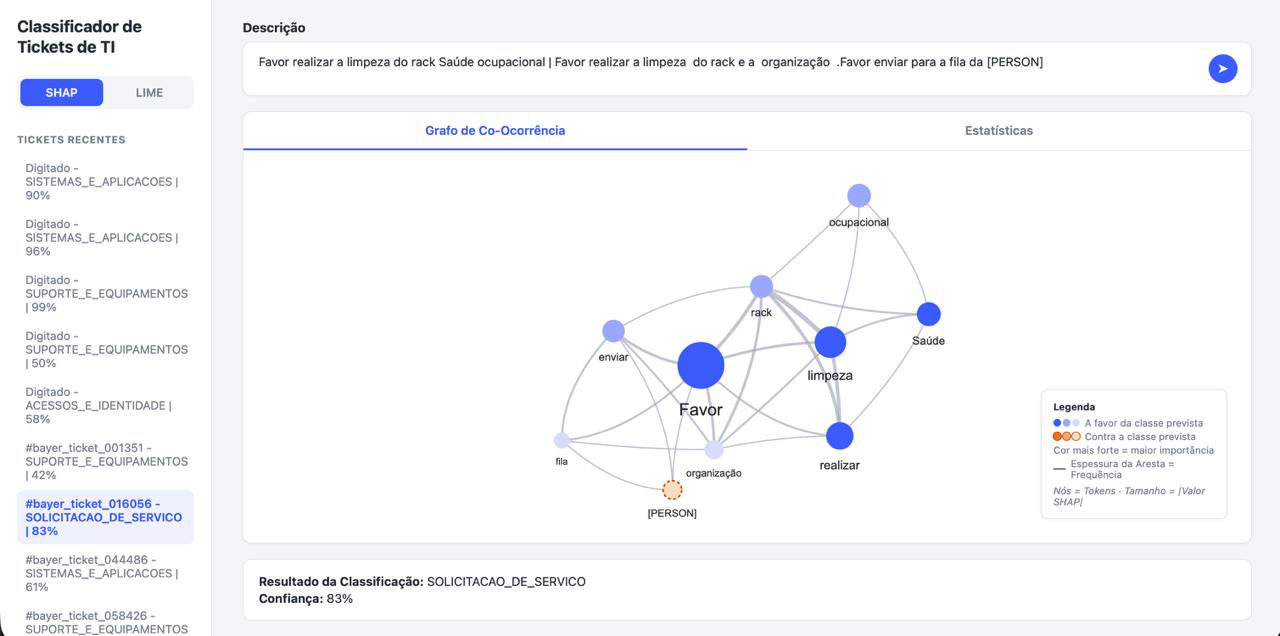
\includegraphics[width=\textwidth]{imagens/grafo_caso3_bayer_016056.png}
    \legend{Fonte: Elaborado pelos autores}
\end{figure}

\section{Análise crítica e comparação}
\textbf{Classificação.} O BERTimbau superou o \textit{baseline} SVM em 3,7 pontos percentuais de F1-macro (intervalo de 95\% de 1,0 a 6,7), abaixo do critério de 5 pontos do TCC1. Os dados mostram que o ganho existe, mas não que ele atinja o critério: o intervalo inclui o 5, e a probabilidade de a diferença verdadeira ser de pelo menos 5 pontos é de cerca de 21\%. O ganho vem da revocação e se concentra em poucas classes (SOFTWARE e SOLICITACAO\_DE\_SERVICO, além de duas classes pequenas), enquanto na maior classe os dois modelos empatam. Há ainda dois cuidados de leitura: o resultado na Aché é pouco informativo, pois seus chamados formam poucos grupos de texto, e na validação um único texto repetido 491 vezes inflaria a diferença para 11,9 pontos. Por isso, o resultado mais seguro é o do teste, com os grupos de texto reamostrados juntos.
 
\textbf{Fidelidade.} O SHAP e o LIME têm fidelidade bem acima do acaso, e a comparação chamado a chamado não distingue os métodos na \textit{comprehensiveness} nem na \textit{sufficiency}. Só no Tau-LOO há diferença, a favor do LIME (diferença média de $-$0,059 para o SHAP, com intervalo que exclui o zero). Isso difere do que se poderia esperar de um método com garantias teóricas como o SHAP, mas uma diferença em uma das três medidas não basta para afirmar que o LIME seja mais fiel.
 
\textbf{Estabilidade.} \citeonline{salih2023} indicam que o SHAP tende a ser mais estável que o LIME. Neste trabalho, isso só vale quando o SHAP é calculado de forma exata, o que ocorre em textos curtos (até 10 palavras por campo), onde a explicação é idêntica em todas as repetições. Nos 9 chamados em que o SHAP foi estimado por amostragem, com orçamento de 500 consultas, o LIME foi mais estável (mesma palavra no topo em 93\% das repetições, contra 68\%). Uma explicação possível, que este trabalho não testou, é que 500 consultas são poucas para textos longos; o orçamento, portanto, é um parâmetro que troca tempo de processamento por estabilidade, e o resultado vale para o orçamento usado. A amostra de 12 chamados é pequena, e as conclusões são indicativas.
 
\textbf{Concordância.} Os dois métodos concordam bem acima do acaso (a mesma palavra no topo em 71\% dos chamados), mas a concordância cai com o tamanho do texto. Assim, em chamados longos, a escolha do método muda de forma relevante quais palavras o analista vê como importantes.
 
\textbf{Grafo.} Nos três estudos de caso, a rastreabilidade se cumpriu: cada nó e cada aresta puderam ser levados ao chamado e aos pesos do SHAP e do LIME. Os casos também mostraram o uso prático da explicação: no caso 2, ela expôs que um erro do modelo se apoiou em muito pouca evidência e em um marcador de anonimização, e no caso 3, que os dois métodos concordam na palavra de maior peso, mas destacam palavras diferentes depois dela. A limitação é que três casos, escolhidos para ilustrar situações diferentes, mostram que o grafo é rastreável, mas não que ele melhore a decisão de um analista.

\section{Discussão}
A hipótese de pesquisa (Seção~\ref{sec:hipotese_pesquisa}) tem duas partes, e os resultados as sustentam de forma diferente. A primeira afirma que o grafo ponderado pelos valores SHAP e LIME contribui para a auditabilidade ao permitir rastrear os termos que levaram à categoria. Essa parte foi sustentada nos termos em que foi definida, a rastreabilidade, nos três estudos de caso. Como a auditabilidade foi medida por rastreabilidade e não em um teste com analistas, o resultado mostra que o caminho da decisão pode ser reconstruído, e não que um analista o reconstrua com facilidade.
 
A segunda parte afirma que o SHAP e o LIME produzem explicações com fidelidade e estabilidade distintas. Na fidelidade, a diferença é pequena e só aparece em uma das três medidas, a favor do LIME. Na estabilidade, a diferença depende de como o SHAP é calculado: ele é perfeitamente estável quando exato e menos estável que o LIME quando estimado por amostragem com 500 consultas. A parte é, portanto, sustentada de forma condicional, e o resultado não sustenta a ideia de que um método seja melhor em todos os casos.
 
Em relação aos objetivos específicos, o ganho do BERTimbau sobre o \textit{baseline} foi analisado (3,7 pontos, abaixo do critério de 5), e SHAP e LIME foram comparados em fidelidade, estabilidade e concordância. A consistência semântica das explicações foi avaliada apenas de forma qualitativa, nos casos: no caso 1, as palavras de maior peso (\textit{licença} e \textit{office}) são o vocabulário esperado para a classe, e no caso 2 a explicação mostra uma previsão apoiada em muito pouca evidência. \citeonline{razma2026} observam que o \textit{fine-tuning} de um modelo como o BERT pode destacar termos coerentes com o significado do chamado; os casos analisados aqui mostram que isso ocorre em alguns chamados, mas não em todos.
 
Para a prática de suporte, os resultados sugerem que o grafo é mais útil como ferramenta de auditoria dos erros e das previsões de baixa confiança, como no caso 2, do que como justificativa de todos os acertos. Por fim, os resultados valem para os dados e a configuração usados (duas empresas, um treinamento, uma amostra de 98 chamados), e as limitações descritas no Capítulo~\ref{cap:conclusao} delimitam o alcance das conclusões.

% ===============================================================
% CAPÍTULO 6 - CONCLUSÃO
% ===============================================================
\chapter{Conclusão}
\label{cap:conclusao}

\section{Retomada do problema e dos objetivos}
Este trabalho partiu de um problema: classificadores baseados em \textit{transformers} acertam bem a categoria de um chamado de TI, mas não mostram por que a escolheram, o que dificulta a auditoria de suas decisões. A pergunta de pesquisa foi como se comparam o SHAP e o LIME quanto à fidelidade e à estabilidade das explicações de um classificador BERTimbau, e de que forma um grafo de co-ocorrência contribui para tornar o processo de classificação auditável.

Para respondê-la, os chamados de duas empresas (53.279 chamados, em 11 categorias) foram usados para treinar um \textit{baseline} SVM com TF-IDF e ajustar o BERTimbau, e as decisões do BERTimbau foram explicadas por SHAP e LIME e representadas em um grafo. Os resultados, por objetivo específico, foram os seguintes.

\begin{enumerate}
    \item \textbf{Ganho do BERTimbau sobre o \textit{baseline}.} O BERTimbau obteve F1-macro de 0,628 contra 0,591 do SVM, uma diferença de 3,7 pontos percentuais (intervalo de confiança de 95\% de 1,0 a 6,7), abaixo do critério de 5 pontos definido no TCC1. O ganho existe, mas os dados não mostram que atinja o critério, e ele se concentra em poucas classes.

    \item \textbf{Comparação entre SHAP e LIME.} Em 98 chamados, os dois métodos tiveram fidelidade bem acima do acaso e não se distinguiram na \textit{comprehensiveness} nem na \textit{sufficiency}; só o Tau-LOO foi maior no LIME. Na estabilidade, o SHAP foi perfeito quando calculado de forma exata, mas menos estável que o LIME quando estimado por amostragem com 500 consultas. Os dois apontaram a mesma palavra no topo em 71\% dos chamados, e a concordância caiu com o tamanho do texto.

    \item \textbf{Auditabilidade pelo grafo.} Nos três estudos de caso, cada nó e cada aresta puderam ser levados ao chamado e aos pesos do SHAP e do LIME, o que atende à auditabilidade nos termos em que foi definida, a rastreabilidade. Não se mediu, porém, se analistas conseguem acompanhar a decisão a partir do grafo.

    \item \textbf{Consistência semântica.} Foi avaliada apenas de forma qualitativa, nos casos: em um deles, as palavras de maior peso são o vocabulário esperado para a classe, e em outro a explicação expôs uma previsão apoiada em muito pouca evidência.
\end{enumerate}

Assim, a hipótese de pesquisa foi sustentada na parte da rastreabilidade e, na parte da comparação entre os métodos, de forma condicional: nenhum dos dois foi melhor em todas as medidas.

\section{Contribuições para a Computação}
As contribuições deste trabalho para a área são as seguintes.
 
\begin{itemize}
    \item \textbf{Comparação empírica entre SHAP e LIME em chamados de TI em português.} A literatura identificada não traz essa comparação para um BERT \textit{fine-tuned} em chamados de suporte em português brasileiro. Os resultados mostram que a vantagem de estabilidade atribuída ao SHAP depende de como ele é calculado, e que a escolha do método importa mais em textos longos.
 
    \item \textbf{Protocolo de avaliação das explicações.} O trabalho reúne, em um mesmo procedimento, medidas de fidelidade, estabilidade e concordância, cada uma comparada ao valor esperado ao acaso, com intervalos de confiança por \textit{bootstrap} pareado. O procedimento pode ser reaplicado a outros classificadores de texto.
 
    \item \textbf{Grafo de co-ocorrência com pesos SHAP e LIME como camada de auditabilidade.} O grafo liga cada decisão às palavras do chamado, à janela de co-ocorrência e aos pesos dos dois métodos, e foi implementado em uma interface \textit{web} que serve de prova de conceito.
 
    \item \textbf{Evidência sobre o BERTimbau frente a um \textit{baseline} clássico.} O trabalho mede o ganho do modelo neural em chamados reais de duas empresas, com a divisão dos dados agrupada pelo texto do chamado, de modo que textos repetidos não vazem entre treino e teste, e mostra como textos muito repetidos podem inflar a diferença entre os modelos.
\end{itemize}

\section{Limitações e trabalhos futuros}
Este trabalho tem limitações que delimitam o alcance de seus resultados.

Quanto aos dados, os chamados vêm de apenas duas empresas do setor farmacêutico, e a Bayer reúne 86\% do conjunto de teste. Os chamados da Aché cobrem um único mês (abril de 2026) e têm muitos textos repetidos: os 716 chamados de teste dessa empresa formam apenas 337 grupos de texto, de modo que o resultado na Aché traz menos informação do que o número de chamados sugere. A classe OUTROS tem apenas 12 chamados no teste e nenhum foi acertado, então o desempenho nela não pôde ser avaliado de forma conclusiva. As categorias das duas empresas foram harmonizadas em uma taxonomia única, e os resultados dependem dessa escolha.

Além disso, dos 189.909 chamados da Bayer que restaram após a limpeza, 143.325 não estavam em português e foram descartados pelo filtro de idioma, e não traduzidos; traduzi-los poderia ampliar a base, ao custo de introduzir ruído de tradução no vocabulário técnico.

Quanto à classificação, os resultados vêm de um único treinamento do BERTimbau (semente 42), sem repetição com outras sementes. O intervalo de confiança da diferença para o \textit{baseline} SVM (de 1,0 a 6,7 pontos) inclui tanto ganhos pequenos quanto o critério de 5 pontos, e cerca de 10,2\% dos pares de texto ultrapassam o limite de 256 \textit{tokens}, de modo que o trecho excedente não chega ao modelo.

Quanto à escolha do modelo, o trabalho usou o BERTimbau, um modelo de 2020, e não avaliou modelos generalistas mais recentes (LLMs), nem abordagens com recuperação de contexto (RAG, \textit{Retrieval-Augmented Generation} -- Geração Aumentada por Recuperação) ou explicações em texto geradas pelo próprio modelo, como as de \textit{Chain-of-Thought} (Cadeia de Raciocínio). O BERTimbau foi mantido por ser específico para o português e por permitir calcular, em máquinas locais, as centenas de consultas ao modelo que o SHAP e o LIME exigem por explicação; com um LLM, esse custo seria bem maior. Já as explicações em texto de um LLM teriam de ter sua fidelidade ao processo de decisão avaliada com medidas como as usadas aqui.

Quanto às explicações, o SHAP e o LIME foram avaliados em uma amostra de 98 chamados, e a estabilidade em apenas 12 deles, explicados 5 vezes cada e escolhidos entre os que têm ao menos oito palavras distintas, o que impede estender esse resultado a chamados curtos. Em 79 dos 166 campos explicados, o SHAP foi estimado por amostragem, com orçamento de 500 consultas, o mesmo número de amostras do LIME; orçamentos maiores podem alterar a estabilidade medida. Em alguns chamados, o modelo linear local do LIME ajusta pouco o comportamento do classificador (o $R^2$ local teve mediana de 0,68 e mínimo de 0,11). Além disso, as medidas de fidelidade foram implementadas pelos autores, seguindo a definição de \citeonline{attanasio2023}, e por isso seus valores podem não ser diretamente comparáveis aos de estudos que usam a biblioteca \textit{ferret}.  A fidelidade e a estabilidade não foram calculadas para o SVM, que é interpretável por construção, e a comparação das explicações entre os cenários A e B fica como trabalho futuro.

Quanto ao grafo, a auditabilidade foi avaliada pela rastreabilidade, em estudos de caso, e não em um teste com analistas de TI. O trabalho, portanto, mostra que cada nó e cada aresta podem ser levados de volta ao chamado, mas não que analistas conseguem, na prática, acompanhar a decisão do classificador a partir do grafo.

Como trabalhos futuros, sugerem-se: (i) repetir o treinamento com outras sementes e incluir chamados de outras empresas e de períodos mais longos; (ii) explicar uma amostra maior de chamados, com mais amostras e consultas por explicação, para medir a estabilidade com mais precisão; (iii) avaliar o grafo em um teste com analistas de TI; (iv) comparar o grafo ponderado por SHAP e por LIME com outras formas de apresentar as explicações; e (v) comparar o BERTimbau com modelos generalistas mais recentes e avaliar abordagens com RAG e explicações por cadeia de raciocínio.

% ---------------------------------------------------------------
% ELEMENTOS PÓS-TEXTUAIS
% ---------------------------------------------------------------
\postextual

% ===============================================================
% CAPÍTULO 4 - REFERÊNCIAS BIBLIOGRÁFICAS
% ===============================================================
\bibliography{bibliografia}
\bibliographystyle{abntex2-alf}
% ---------------------------------------------------------------
% APÊNDICES (se necessário)
% ---------------------------------------------------------------
\begin{apendicesenv}
\partapendices

\chapter{Cronograma de atividades}
\label{ap:cronograma}

O cronograma a seguir apresenta as fases do TCC2, com as datas em que foram concluídas e o status atual.

\begin{table}[htb]
  \centering
  \caption{Cronograma do TCC2, com datas e status}
  \label{tab:cronograma}
  \small
  \begin{tabular}{p{4.2cm}p{4.6cm}p{3.6cm}}
    \toprule
    Fase & Período & Status \\
    \midrule
    1. Dados e modelo & setembro a 04/10/2026 & Concluída (modelo final treinado em 04/10) \\
    2. XAI e grafo & outubro a 01/11/2026 & Concluída (rodada oficial do SHAP e do LIME em 01/11) \\
    3. Sistema e interface & até 05/11/2026 & Concluída (prova de conceito funcionando em 05/11) \\
    4. Escrita do documento & 02/11 a 07/11/2026 & Concluída (capítulos 1 a 6 redigidos) \\
    5. Prévia e entrega & 10/11 e 24/11/2026 & Prévia da banca e entrega final agendadas \\
    \bottomrule
  \end{tabular}
  \legend{Fonte: Elaborado pelos autores. Em relação ao plano inicial, a interface passou a ser servida com \textit{Flask}, em vez de \textit{FastAPI}.}
\end{table}

\end{apendicesenv}

% ---------------------------------------------------------------
% ANEXOS (se necessário)
% ---------------------------------------------------------------
\begin{anexosenv}
\partanexos

\chapter{Autorização de uso de dados --- Aché Laboratórios Farmacêuticos}
\label{an:autorizacao_ache}

Troca de e-mails em que a Aché Laboratórios Farmacêuticos, por meio de sua equipe de suporte de TI e do prestador do serviço, concorda em compartilhar a base de chamados de suporte técnico para fins acadêmicos neste trabalho. Nomes, endereços de e-mail, telefones e assinaturas dos participantes foram ocultados, mantendo-se a data, o assunto e o conteúdo da conversa. As mensagens aparecem em ordem cronológica: o pedido dos autores e a concordância da empresa (Figura~\ref{fig:autorizacao_ache_1}) e o envio da base de chamados (Figura~\ref{fig:autorizacao_ache_2}).

\begin{figure}[H]
    \caption{Autorização de uso de dados concedida pela Aché Laboratórios Farmacêuticos (1 de 2): pedido e concordância}
    \label{fig:autorizacao_ache_1}
    \centering
    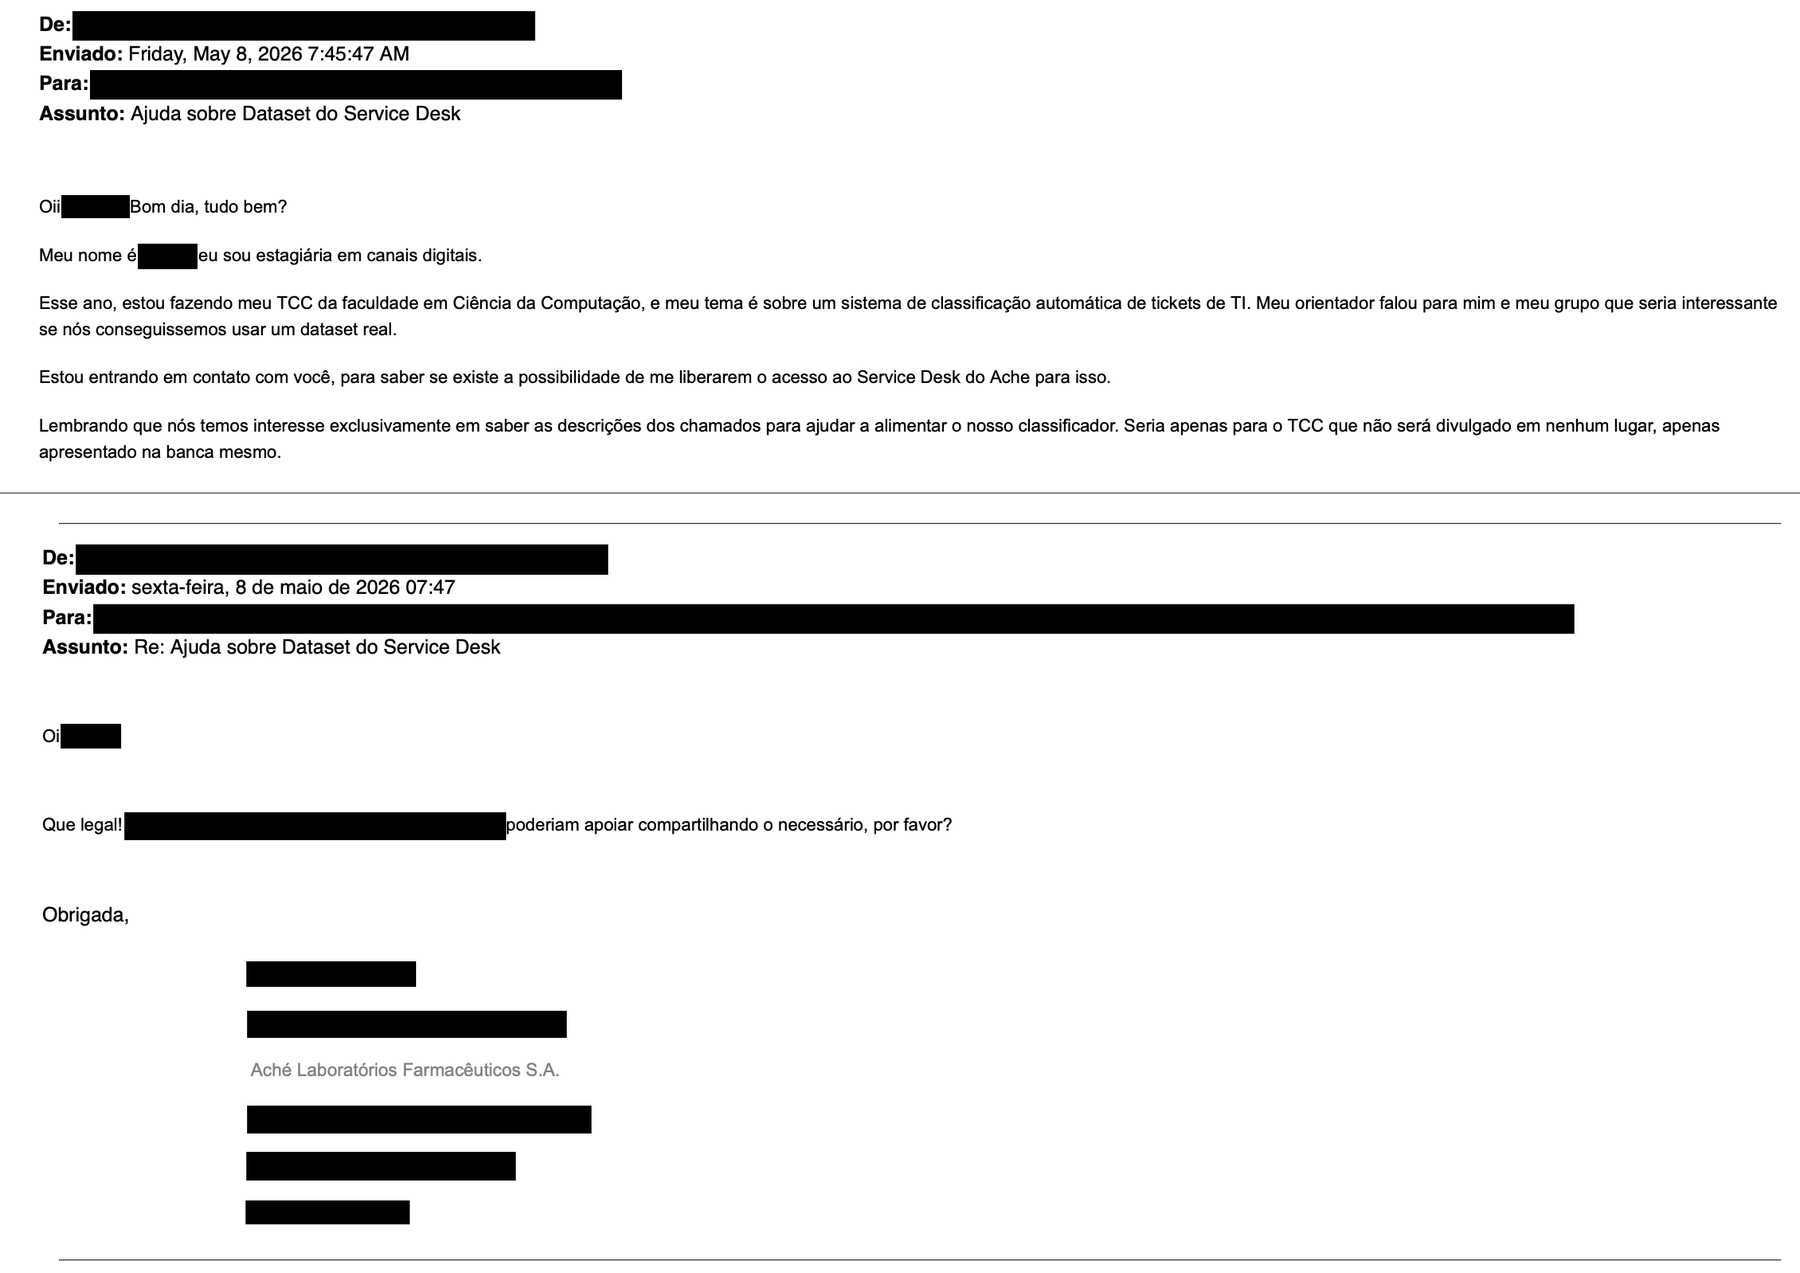
\includegraphics[width=0.9\textwidth]{imagens/autorizacao_ache_1.png}
    \legend{Fonte: Correspondência recebida pelos autores (2026)}
\end{figure}

\begin{figure}[H]
    \caption{Autorização de uso de dados concedida pela Aché Laboratórios Farmacêuticos (2 de 2): acompanhamento e envio da base}
    \label{fig:autorizacao_ache_2}
    \centering
    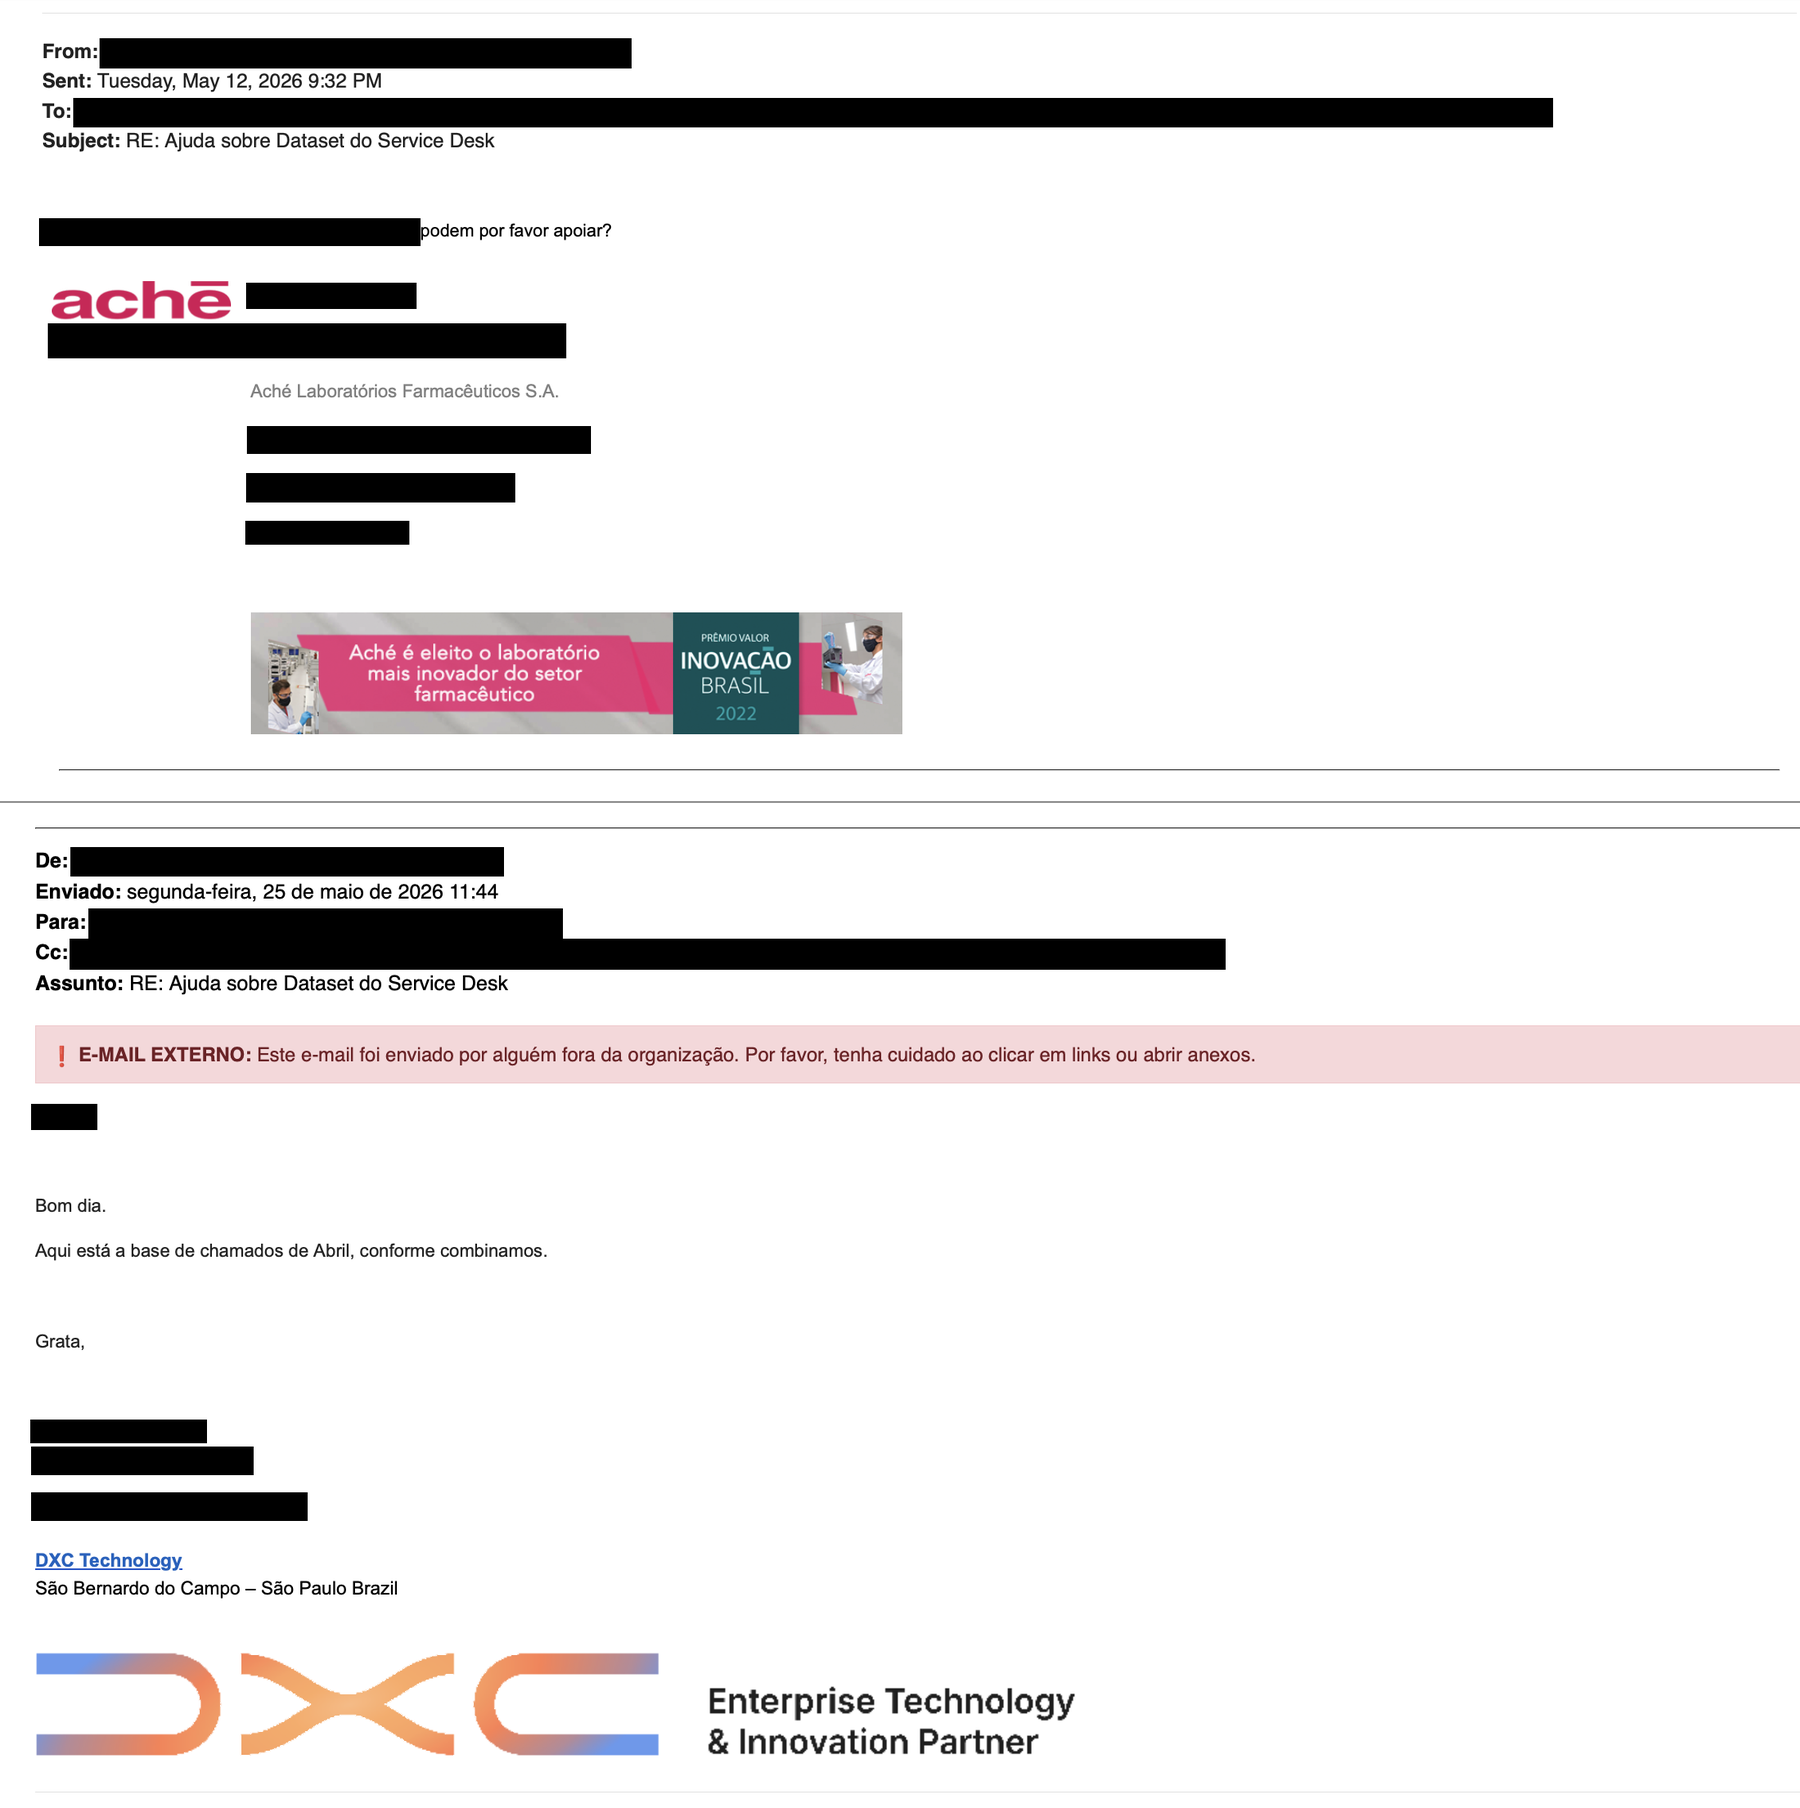
\includegraphics[width=0.9\textwidth,height=0.75\textheight,keepaspectratio]{imagens/autorizacao_ache_2.png}
    \legend{Fonte: Correspondência recebida pelos autores (2026)}
\end{figure}

\chapter{Autorização de uso de dados --- Bayer S.A.}
\label{an:autorizacao_bayer}

Mensagem de e-mail em que a Bayer S.A. autoriza o uso de chamados de
suporte técnico para fins acadêmicos neste trabalho, mediante
anonimização dos registros. Nomes, e-mails, ramais e assinaturas dos
remetentes foram removidos da imagem, mantendo-se apenas o conteúdo da
autorização e a identificação da empresa.

\begin{figure}[H]
    \caption{Autorização de uso de dados concedida pela Bayer S.A.}
    \label{fig:autorizacao_bayer}
    \centering
    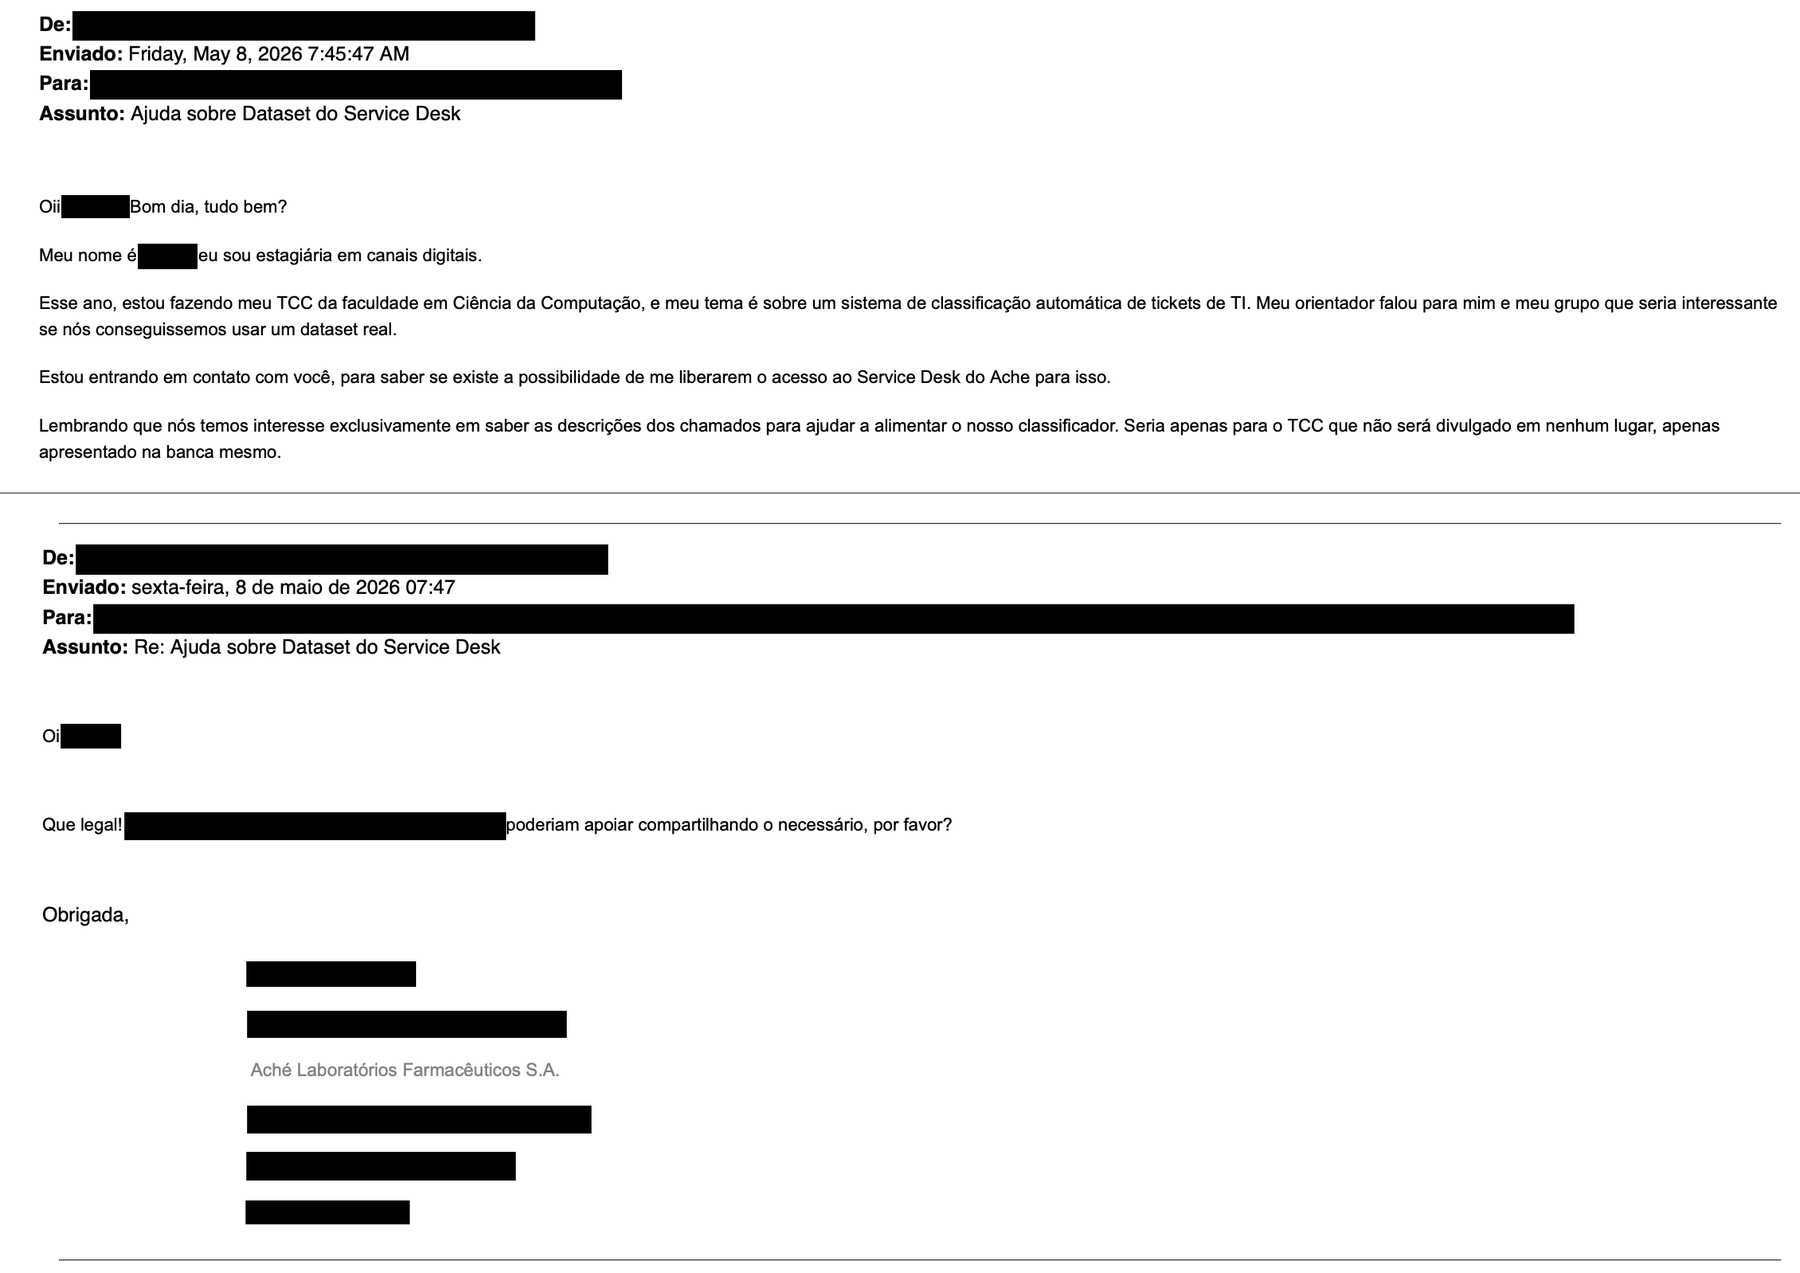
\includegraphics[width=0.85\textwidth]{imagens/autorizacao_bayer.png}
    \legend{Fonte: Correspondência recebida pelos autores (2026)}
\end{figure}

\end{anexosenv}
% ---------------------------------------------------------------
% ANEXOS
% ---------------------------------------------------------------



\end{document}